\documentclass[twoside]{article}
\setlength{\oddsidemargin}{0.25 in}
\setlength{\evensidemargin}{-0.25 in}
\setlength{\topmargin}{-0.6 in}
\setlength{\textwidth}{6.5 in}
\setlength{\textheight}{8.5 in}
\setlength{\headsep}{0.75 in}
\setlength{\parindent}{0 in}
\setlength{\parskip}{0.1 in}

%
% ADD PACKAGES here:
%
\usepackage[ruled,vlined]{algorithm2e}
\usepackage{amsmath,amsfonts,amssymb,graphicx,mathtools,flexisym, hyperref, graphicx}
\graphicspath{ {./Images/} }

\usepackage{tcolorbox}

%
% The following commands set up the lecnum (lecture number)
% counter and make various numbering schemes work relative
% to the lecture number.
%
\newcounter{lecnum}
\renewcommand{\thepage}{\thelecnum-\arabic{page}}
\renewcommand{\thesection}{\thelecnum.\arabic{section}}
\renewcommand{\theequation}{\thelecnum.\arabic{equation}}
\renewcommand{\thefigure}{\thelecnum.\arabic{figure}}
\renewcommand{\thetable}{\thelecnum.\arabic{table}}
\newcommand{\utilde}{\underset{\sim}}
\newcommand{\prob}{\mathbb{P}}
%
% The following macro is used to generate the header.
%
\newcommand{\lecture}[4]{
   \pagestyle{myheadings}
   \thispagestyle{plain}
   \newpage
   \setcounter{lecnum}{#1}
   \setcounter{page}{1}
   \noindent
   \begin{center}
   \framebox{
      \vbox{\vspace{2mm}
    \hbox to 6.28in { {\bf DATA5441: Networks and High-dimensional Inference
    \hfill } }
       \vspace{4mm}
       \hbox to 6.28in { {\Large \hfill #1. #2 \hfill} }
       \vspace{4mm}
       }
   }
   \end{center}


}
%
% Convention for citations is authors' initials followed by the year.
% For example, to cite a paper by Leighton and Maggs you would type
% \cite{LM89}, and to cite a paper by Strassen you would type \cite{S69}.
% (To avoid bibliography problems, for now we redefine the \cite command.)
% Also commands that create a suitable format for the reference list.
\renewcommand{\cite}[1]{[#1]}
\def\beginrefs{\begin{list}%
        {[\arabic{equation}]}{\usecounter{equation}
         \setlength{\leftmargin}{2.0truecm}\setlength{\labelsep}{0.4truecm}%
         \setlength{\labelwidth}{1.6truecm}}}
\def\endrefs{\end{list}}
\def\bibentry#1{\item[\hbox{[#1]}]}

%Use this command for a figure; it puts a figure in wherever you want it.
%usage: \fig{NUMBER}{SPACE-IN-INCHES}{CAPTION}
\newcommand{\fig}[3]{
            \vspace{#2}
            \begin{center}
            Figure \thelecnum.#1:~#3
            \end{center}
    }
% Use these for theorems, lemmas, proofs, etc.
\newtheorem{theorem}{Theorem}[lecnum]
\newtheorem{lemma}[theorem]{Lemma}
\newtheorem{proposition}[theorem]{Proposition}
\newtheorem{claim}[theorem]{Claim}
\newtheorem{corollary}[theorem]{Corollary}
\newtheorem{definition}[theorem]{Definition}
\newtheorem{remark}[theorem]{Remark}
\newtheorem{example}[theorem]{Example}
\newenvironment{proof}{{\bf Proof:}}{\hfill\rule{2mm}{2mm}}

\graphicspath{ {./Images/} }

\tcbuselibrary{theorems}
\newtcbtheorem
  []% init options
  {theorem_exam}% name
  {Theorem}% title
  {%
    colback=orange!5,
    colframe=orange!35!black,
    fonttitle=\bfseries,
  }% options
  {def}% prefix


\newtcbtheorem
  []% init options
  {definition_exam}% name
  {Definition}% title
  {%
    colback=blue!5,
    colframe=blue!35!black,
    fonttitle=\bfseries,
  }% options
  {def}% prefix  


\newtcbtheorem
  []% init options
  {proposition_exam}% name
  {Proposition}% title
  {%
    colback=red!5,
    colframe=red!35!black,
    fonttitle=\bfseries,
  }% options
  {def}% prefix  

\newcommand{\Lim}[1]{\raisebox{0.5ex}{\scalebox{0.8}{$\displaystyle \lim_{#1}\;$}}}
\newcommand{\Inf}[1]{\raisebox{0.5ex}{\scalebox{0.8}{$\displaystyle \inf_{#1}\;$}}}
\newcommand{\Sup}[1]{\raisebox{0.5ex}{\scalebox{0.8}{$\displaystyle \sup_{#1}\;$}}}
\newcommand{\norm}[1]{\left\lVert#1\right\rVert}
%
% To generate a clickable table of content.
%
\hypersetup{
    colorlinks,
    citecolor=black,
    filecolor=black,
    linkcolor=blue,
    urlcolor=black
}


\newcommand\E{\mathbb{E}}
\usepackage{tocloft}

\addtolength{\cftsecnumwidth}{10pt}
\setlength{\cftsubsecnumwidth}{3.5em}

\title{DATA5441: Networks and High-dimensional Inference}
\author{Charles Christopher Hyland}
\date{Semester 1 2020}


\begin{document}

\pagenumbering{gobble}
\maketitle
\begin{abstract}
Thank you for stopping by to read this. These are notes collated from lectures and tutorials as I took this course.
\end{abstract}
\newpage
\tableofcontents
\newpage
\pagenumbering{arabic}


\lecture{1}{Network Theory Definitions}
\section{Network Theory Definitions}
\section{Network Theory Definitions}
\subsection{Why study networks?}
There are two main reasons on why we study networks. First, is that networks are useful as models of real world phenomena. Furthermore, networks are paradigms of data science in 3 aspects:
\begin{enumerate}
\item Large, noisy, and inter-dependent data;
\item Tension between models, methods, and real data;
\item Large search/sample/inference spaces.
\end{enumerate}

\subsection{Network Theory Introduction}
We define $\mathcal{N}$ to be a set of n = 1,2,..., N  \textbf{nodes.} We define $\mathcal{L}$ to be a set of l = 1,2,..., L \textbf{links}. \\

\begin{definition_exam}{Network}{} If all $l_i \in \mathcal{L}$ are such that $l_i = \{n_j,n_k\}$ with $n_j,n_k \subset \mathcal{N}$, we say that this builds a network.
\end{definition_exam}

We have three representations of a network.


1) \textbf{Graphical}: We can use basic graph theory to label nodes as vertices and edges as links.\newline 
2) \textbf{Adjacency matrix}: We have a $N \times N$ matrix whereby we have for the entries in the matrix 
$$
A_{ij} = 
\begin{cases}
1 \quad \text{if there is } \ell_i = \{n_i, n_j\}\\
0 \quad \text{otherwise.}
\end{cases}
$$
3) \textbf{List of links}: We have a set containing the links $\mathcal{L} = \{l_1,l_2,...,l_L\}$

\begin{remark}In most real world networks, adjacency matrices are usually sparse (most entries are zeros). Hence, it is better for memory to store the network as a list of links.
\end{remark}

We now look at some examples of networks.
\begin{definition}(Lattice). Start with the points $\mathbb{Z}^d$ as nodes. We then link all nodes within a certain lattice distance $\omega.$
\end{definition}

\begin{definition}(Tree). A tree is a connected acyclic graph.
\end{definition}

\begin{definition}(Complete graph). A complete graph is a simple undirected graph in which every pair of distinct vertices is connected by a unique edge.
\end{definition}

We will now show that the number of simple graphs that exist in a network with N nodes grows exponentially.

\begin{proposition_exam}{Number of potential links}{}For a N dimensional network, there are $\frac{N(N-1)}{2}$ possible links in the network.
\end{proposition_exam}

From this, we can now define the size of the sample space.

\begin{proposition_exam}{Number of potential networks}{}The size of the sample space for a N dimensional network is 
$$
|\Omega| = 2^{\frac{N(N-1)}{2}} \approx 2^{N^{2}}
$$
\end{proposition_exam}
\begin{proof} In the $N \times N$ adjacency matrix, we only need to look at the upper diagonal matrix due to symmetry. There are $\frac{N(N - 1)}{2}$ entries that will either have a 0 or a 1.
\end{proof}

Hence, we can see that the sample space is massive. Therefore, we will require smart tools in order to examine such models.

\begin{definition}(Eulerian path). A Eulerian path is a path that visits every link \textbf{exactly once}.
\end{definition}

\begin{lemma}(Königsberg Bridge Problem). For an Eulerian path to exist in a network, the number of nodes with odd number of links is either 0 or 2.
\end{lemma}

In complex networks, there are similar structures between different networks. Furthermore, there is an interesting interaction between the structure (topology) of the network and the function (dynamics) defined on the network, which we will explore later in this course.

\lecture{2}{Network Measures}
\section{Network Theory Definitions}
\subsection{Network Measures}

We are interested in two types of measures, local and global measures. Local measures quantify the property of a given node or link whereas global measure looks at the network as a whole.

Suppose we have a network with N nodes and an associated adjacency matrix. We give the form of the adjacency matrix for different types of networks.

\begin{enumerate}
\item \textbf{Simple graphs}: the adjacency matrix $A_{ij} = \begin{cases}0\\1\end{cases}$ depending on whether is there a link between node i and j.
\item \textbf{Directed networks}: we have that $A_{ij} \neq A_{ji}$.
\item \textbf{Multigraphs}: we have that $A_{ij} \in \mathbb{N}.$
\item \textbf{Weighted networks}: we have that $A_{ij} \in \mathbb{R}.$
\item \textbf{Layered networks}: we have multiple types of links between nodes.
\item \textbf{Temporal networks}: links now have time stamps.
\item \textbf{Bipartite networks}: we have 2 types of nodes.
\end{enumerate}

We now start to define network measures.

\begin{definition_exam}{Path}{} A path is any sequence of nodes $\{n_1, n_2, ..., n_r\}$ such that every consecutive pair of nodes is connected by a link $l = \{n_i, n_{i + 1}\} \in \mathcal{L}$ for all $1 \leq i < r$. The length of a path is the \textbf{number of links} in the sequence.
\end{definition_exam}

\begin{claim}The number of paths of length r between node i and j, which we denote by $N_{i,j}^r$ is given by 
$$
N_{i,j}^r = [A^r]_{i,j} = [A \cdot \cdot \cdot A]_{i,j}
$$
where A is the adjacency matrix and $[]_{i,j}$ denotes the entry at (i,j).
\end{claim}

\begin{proof} We can prove this by induction. Let $r = 1.$ Then, the number of paths of length 1 between i and node j is given by 
$$
N_{i,j}^{1} = A_{ij}
$$
Now, let r = 2. Then, we need to think about transitive nodes k which may be between node i and j. Therefore 
$$
N_{i,j}^{2} = \sum_{k}A_{ik}A_{kj} = [A^2]_{ij}
$$
We can extend this to hold for any arbitrary path of length r.
\end{proof}

\begin{definition_exam}{Shortest geodesic path}{} We define the shortest geodesic path $d_{ij}$ between node i and node j to be the shortest length path between node i and node j. Alternatively, it is the minimum r such that $N_{i,j}^r \neq 0.$
\end{definition_exam}

\begin{definition}(Closed path). A closed path is a path where the initial and final node are the same.
\end{definition}

\begin{definition}(Neighbourhood). The neighbourhood of a node i is the set of all nodes j that have $d_{ij} = 1.$
\end{definition}

We are now interested in the notion of the distance of a path. This is a measure which we will repeatedly use throughout the course.

\begin{definition_exam}{Local Measure of Path Distance}{}We define the local measure of a path distance for node i as 
$$
d_i = <d_{ij}>_j = \frac{1}{N-1}\sum_{\substack{n=1\\ n \neq i}}^{N}d_{i,n}
$$
where we look at how close a node i is to every other node in the network.
\end{definition_exam}
\begin{remark}This calculation assumes the network is one \textbf{connected component}.
\end{remark}

\begin{definition_exam}{Global Measure of Path Distance}{}We define the global measure for a network with N nodes as 
$$
d = <d_i>_i = \frac{1}{N}\sum_{n=1}^{N}d_n.
$$
\end{definition_exam}

As we will come to see later, it is a common propety to see that despite the large sizes of networks, there is relatively short distances between any two pair of nodes. However, it is important to be wary of this as we will see later that short distances can be explained just through random graphs.

\begin{definition_exam}{Connected component}{} All nodes for which $d_{ij} < \infty$ defines a connected component.
\end{definition_exam}

\newpage
We now define another measure of interest which we will use repeatedly through the course.

\begin{definition_exam}{Degree of a node}{}The degree of node i, denoted by $z_i$, is defined to be the number of links node i has. Alternatively, it is defined to be the size of the neighbourhood of node i.
\end{definition_exam}

\begin{definition_exam}{Average degree of network}{} The average degree of nodes in a network of size N is given by 
 $$
<Z> = \frac{1}{N}\sum_{n=1}^{N}z_n = \frac{2L}{N}
$$
where L is the total number of links in the network.
\end{definition_exam}

\begin{claim} The number of links in an undirected network is 
$$
L = \frac{1}{2}\sum_{n=1}^{N}z_n
$$
where $z_n$ is the degree of node n.
\end{claim}

We are now able to define more precisely what happens when we take limits within networks.

\begin{definition_exam}{Sparse network}{} A network is sparse if most entries of the adjacency matrix $A_{ij} = 0.$
\end{definition_exam}

From this, we can give a new interpretation of what it means for a network to be sparse.

\begin{proposition_exam}{Characterisation of a sparse network}{}A network is sparse if $$\langle Z \rangle \rightarrow K$$ when $N \rightarrow \infty$ where K is a constant and $\langle Z \rangle$ is the average degree of the network.
\end{proposition_exam}
\begin{proof} First, the number of entries in the adjacency matrix $A_{ij} = 0$ is proportional to $A_{i,j} = \frac{N(N - 1)}{2} \sim N^2$, which denotes the number of possible links that can be created. As 
$$
\langle Z \rangle = \frac{2L}{N}
$$
where L is the number of links and N is the number of nodes in the network, then if 
$$
\langle Z \rangle \rightarrow K
$$
for some constant K, this only happens if the number of links $L \sim N$ and the number of entries $A_{i,j} = 0 \sim \frac{1}{N}$.
\end{proof}

\begin{remark} We do not want the number of links to be a constant as we increase the number of nodes in the network. We want the average degree of the network to stay constant as we increase the number of nodes, which forces the number of links to increase. However, this in fact forces the number of links to increase at a certain rate $\mathcal{O}(N)$ and not any larger in order to keep $\langle Z \rangle$ to be a constant.
\end{remark}

This idea of sparsity matches our intuition that the number of friends that we have does not depend on the total population size. Most of our focus in this course is on sparse networks. As a result, we can also define what it means for a network to be dense.

\begin{proposition_exam}{Characterisation of a dense network}{}A network is dense if $$\langle Z \rangle \rightarrow \infty$$ when $N \rightarrow \infty$ where $\langle Z \rangle$ is the average degree of the network.
\end{proposition_exam}

\subsection{Clustering Coefficient}

A common property of social networks is that cliques form. That is, groups are formed where every member knows every other member, which in the case of networks, is when there is a subgraph where each node has an edge to all other nodes in the subgraph. This inherent tendency to cluster is quantified by the clustering coefficient, which we shall now describe.

We are interested in how "clustered" is our network. Effectively, the clustering coefficient C measures
$$
\mathbb{P}(A_{jk} = 1| A_{ij} = 1, A_{ik} = 1)
$$
where i, j, k are nodes. Hence, this models the probability of forming a triangle in the network.

\begin{claim}(Clustering coefficient of extreme graphs). The clustering coefficient C of a tree is 0. The clustering coefficient of a fully connected network is 1.
\end{claim}

We can now define our first notion of clustering.

\begin{definition_exam}{Local Clustering}{}We define the local measure of clustering for a node i as 
$$
C_i = \frac{\text{\# of neighbours of i that are connected}}{\text{\# of pairs of neighbours}} = \frac{2 \cdot \# \text{ of triangles node i forms}}{z_i(z_i - 1)}
$$
where $z_i$ is the degree of node i.
\end{definition_exam}

\begin{remark} To actually compute $C_i$ for a node i, count how many triangles is node i involved in and look at the degree of node i.
\end{remark}

This is a useful measure of local clustering for node i as if a clique was indeed formed for node i, then for each neighbour of node i, there should be $z_i(z_i - 1)/2$ edges between node i and the neighbours of node i.

Based off the notion of local clustering, we now define two different measures of global clustering.

\begin{definition_exam}{Global Clustering}{}The first global clustering coefficient is taking an average of the local clustering measure
$$
<C> = \frac{1}{N}\sum_{i=1}^NC_i.
$$
The second method of computing the global clustering coefficient
$$
C_{Net} = \frac{\text{number of closed paths of length 3}}{\text{number of path of length 2}} = \frac{\text{3 \# triangles}}{\text{\# of connected triples}}
$$
\end{definition_exam}
\begin{remark} The easiest way to compute $C_{Net}$ is to count the number of paths of length 2 and see how many of them are closed and hence forms a triangle.
\end{remark}

\begin{remark}The global clustering coefficients do not necessarily agree with one another $$C_{Net} \neq \langle C \rangle$$
\end{remark}

\lecture{3}{Centrality Measures}
\section{Network Theory Definitions}
\subsection{Centrality Measures}

With networks, we can compute measures to characterise the nodes or the networks as a whole. We are most interested in the central nodes in the network.

\begin{definition}(Degree). The degree $Z_i$ is the number of edges outgoing from node i.
\end{definition}

\begin{definition_exam}{Hubs}{}The hubs of the network are the nodes with the highest degree.
\end{definition_exam}

\begin{definition}(Average distance). The measure $\langle d_i \rangle$ is the average shortest path for node i. That is, the average of all shortest path distances from node i to the other nodes in the network.
\end{definition}

\begin{definition_exam}{Betweeness Centrality}{}The betweeness centrality of node i, denoted by $B_i$ takes into account the number of shortest paths that node i appears in. Let $\eta_{s,t}^{i}$ be the number of shortest paths between node s and t through node i. Let $g_{s,t}$ be the number of shortest paths between s and t. The betweeness centrality of node i is 
$$
B_i = \sum_{s=1}^N\sum_{t=1}^N\frac{\eta_{s,t}^{i}}{g_{s,t}}.
$$
\end{definition_exam}


\begin{remark}We may have different networks of different sizes whereby we wish to the compare the betweeness centrality across them. The size of the graph grows with $N^2$ so sometimes we define the betweeness centrality as 
$$
\tilde{B}_i = \frac{1}{N^2}\sum_{s,t}\frac{\eta_{s,t}^i}{g_{s,t}}.
$$
\end{remark}

An issue is that none of these measures take into account that if you are close to a central node, then you yourself are a central node. The next few centrality measures take this into account.


The general idea is that each node has a measure of centrality. Then, at each time step, the node passes its centrality onto its neighbours. We then get rid of this time dependence by taking $t \rightarrow \infty.$

First, assume we have a measure of the centrality for each node in our network 
$$
\utilde{x} = (x_1, x_2, ..., x_N)
$$
Now, the state of each node i evolves as follows in one time step
$$
x_i(t + 1) = \sum_{j=1}^{N}A_{ij}x_j(t)
$$
Here, the centrality of node i in the next time step depends on the centrality measure of all of its neighbours. It is worth to note that this implies that if a node is not connected, then its centrality will not change in the next time step.

In vector notation, we can write the state evolution of one time step as
\begin{equation}
\utilde{x}(t + 1) = A\utilde{x}(t)
\tag{*}
\end{equation}

We now have a linear dynamic system, where measures of centrality of each node is evolving according to the matrix A. We now recall an important theorem from linear algebra.
\begin{theorem_exam}{Perron-Frobenius Theorem}{} Let $\lambda_1 \geq \lambda_2 \geq ... \geq \lambda_N$ be the N eigenvalues of the adjacency matrix A and let $\utilde{v_1}, \utilde{v_2}, ..., \utilde{v_N}$ be the corresponding eigenvectors where $\utilde{v_i} \in \mathbb{R}^n$. Suppose that the adjacency matrix A is a square matrix with non-negative entries. Furthermore, assume that A is irreducible, that is, the network is a single connected component.

Then, the eigenvalue $\lambda_1$ where $\lambda_1 \geq \lambda_2 \geq ... \geq \lambda_N$, is real-valued and nonnegative with bounds of 
$$
\min_{i,j}A_{i,j} \leq \lambda_1 \leq \max_i\sum_{j}A_{ij}.
$$
Furthermore, the associated eigenvector $\utilde{v_1}$ of the largest eigenvalue $\lambda_1$ has nonnegative real valued entries whereby 
$$
\utilde{v_1} = 
\begin{bmatrix}
v_{11}\\
v_{12}\\
\cdot \cdot \cdot \\
v_{1i}\\
\cdot \cdot \cdot \\
v_{1N}\\
\end{bmatrix}
$$
\end{theorem_exam}
\begin{remark}In the eigenvector $\utilde{v_1}$, we have an entry for each node in the network.
\end{remark}

Perron-Frobenius gives us the fact that a square matrix with positive entries has a unique eigenvector with positive entries and the corresponding eigenvalue has an aboslute value greater than the absolute value of any other eigenvalue.

We now apply the Perron-Frobenius theorem to our equation (*). 

\begin{theorem} A $N \times N$ real-valued symmetric matrix is diagonalisable.
\end{theorem}

\begin{corollary} A matrix that is diagonalisable can be writen in terms of its eigenvector basis.
\end{corollary}

Using the last 2 results, we can express our centrality measure vector in terms of an eigenvector basis
$$
\utilde{x} = \sum_{i=1}^{N}a_i\utilde{v_i}
$$
Then, we can express the time evolution of our system 
$$
\utilde{x}(t) = A^t\utilde{x}(0) = A^t\sum_{i=1}^{N}a_i\utilde{v_i}(0) = \sum_{i=1}^{N}a_i\lambda_i^t \utilde{v_i}(0)
$$

where the last equality arises as $\utilde{v_i}$ are eigenvectors of the matrix A, that is $A^t\utilde{v_i} = \lambda_i^t\utilde{v_i}$. Then, we multiply and divide through by the largest eigenvalue $\lambda_1$ to get

$$
= \lambda_1^t\sum_{i=1}^{N}a_i\bigg(\frac{\lambda_i}{\lambda_1}\bigg)^t \utilde{v_i}(0)
$$

Now, as $\lambda_1$ was assumed to be the largest eigenvalue, we have that 
$$
\bigg(\frac{\lambda_i}{\lambda_1}\bigg)^t \rightarrow 0
$$
as $t \rightarrow \infty$ for any $i > 1.$ Therefore, we can conclude that the centrality measure vector 
$$
\utilde{x}(t) \propto \lambda_1^t\utilde{v_1}
$$
for $t \rightarrow \infty.$

We can therefore make the following conclusion.

\begin{proposition_exam}{State vector is proportional to largest eigenvector}{}Let $\utilde{x}(t) = (x_1, x_2, ..., x_N)$ be the centrality measure vector of our network of N nodes at time t. Then, as $t \rightarrow \infty,$ we have that 
$$
\utilde{x}(t) \propto \lambda_1^t\utilde{v_1}
$$
where $\lambda_1$ is the largest eigenvalue of the adjacency matrix and $\utilde{v_1} \in \mathbb{R}_{+}^{N}$ is the corresponding eigenvector.
\end{proposition_exam}

We can now define a new centrality measure.

\begin{definition_exam}{Eigenvector centrality}{}The eigenvector centrality of node i is given by 
$$
x_i = v_{1, i}
$$
where $v_{1, i}$ is the i-th component of the largest eigenvector $\utilde{v_1}$ associated to the largest eigenvalue $\lambda_1.$
\end{definition_exam}

\begin{remark}As a result of the Perron-Frobenius theorem, we have that $v_{1,i} \in \mathbb{R}$, which means that the eigenvector centrality $x_i \in \mathbb{R}.$ 
This means we can now rank the eigenvector centrality of all nodes.

Additionally, we also note that the eigenvector centrality
$$
x_i = \frac{1}{\lambda_1}\sum_{j=1}^{N}A_{ij}x_j
$$
is the sum of the centrality of the neighbours.
\end{remark}

Hence, we now have a centrality measure that depends on its neighbours.

However, there are a few issues with eigenvector centrality. First, recall that in directed networks, $A_{ij} \neq A_{ji}.$ The first issue is that nodes that do not have any incoming edges $Z^{in} = 0$, will have a eigenvector centrality of zero as no neighbour is passing their centrality to you.

Furthermore, nodes that have outgoing edges into nodes with eigenvector centrality of 0 will also have an eigenvector centrality of zero, that is, a zero eigenvector centrality can propagate through the network.

From both of these issues, we may have a large number of nodes in our network with an eigenvector centrality of zero, which is not desirable. This motivates our next centrality measure.

Now, we propose a new dynamic for the centrality measure evolution to be 
\begin{equation}
\utilde{x}(t + 1) = \alpha A \utilde{x}(t) + \beta \mathcal{I}
\tag{**}
\end{equation}
where $\alpha, \beta \in \mathbb{R}$ and $\mathcal{I}$ is an unit vector. The intuition is that the centrality measure being passed to neighbours again depends on the neighbours, but now, we are also pumping a certain centrality measure of size $\beta$ at each time step to all nodes. This prevents any node from having a centrality measure of x = 0.

We can now do a similar procedure as earlier.
\begin{lemma}For $t > > 1$, the centrality measure under the linear system (**) is proportional to
$$
\utilde{x}(t + 1) \propto \gamma \utilde{x}(t).
$$
\end{lemma}

\begin{remark}We see that the pumping measure $\beta \mathcal{I}$ has no effect in the limit.
\end{remark}

From this, we can then write 
$$
\gamma \utilde{x} = \alpha A \utilde{x} + \beta \mathcal{I}
$$
$$
\utilde{x}\bigg[\mathbb{I} - \frac{\alpha}{\gamma}A \bigg] = \beta \mathcal{I}
$$
where $\mathbb{I}$ is the identity matrix. We can now define a new centrality measure.

\begin{definition_exam}{Katz Centrality}{}Suppose that the linear dynamic system for the evolution of centrality measure is given by 
$$
\utilde{x}(t + 1) = \alpha A \utilde{x}(t) + \beta \mathcal{I}
$$
where $\alpha, \beta \in \mathbb{R}$, $\utilde{x} \in \mathbb{R}^N$ is the centrality measure for each node i = 1,..., N, and $\mathcal{I}$ is an unit vector.

Then, the Katz centrality measure is defined as 
$$
\utilde{x} = \beta\bigg[\mathbb{I} - \frac{\alpha}{\gamma}A \bigg]^{-1} \mathcal{I}
$$
where $\mathbb{I}$ is the identity matrix and $\gamma$ is a constant.
\end{definition_exam}

\begin{remark}Since we are interested in only the relative values of the Katz centrality measure in order to compare nodes, we can let $\beta = 1$ and $\gamma = 1$ without loss of generality. Therefore, the only constant to set in the Katz centrality measure is $\alpha.$
\end{remark}

However, a big issue with the Katz centrality is that we have an inflation of centrality. The centrality is spread in full to all outgoing links. That is, a website with many hyperlinks to other websites should not expect to pass on its centrality to all its outgoing neighbours. Therefore, we should restrict this. What Page-rank centrality does is to only choose random outgoing links to receive the centrality measure.

This comes up with the idea of the random surfer in the Page-rank algorithm. When we are on a webpage, we will pick one random outgoing link to pass the centrality to. The probability of picking one webpage outgoing from node j is given by $\frac{1}{Z_j^{out}}$. We therefore assume a random walk in the directed network. We can therefore state the Page-rank centrality.

\begin{definition_exam}{Page-rank Centrality}{}The Page-rank centrality is given by 
$$
\utilde{x}(t + 1) = \alpha \sum_{j=1}^N\bigg(A_{ij}\frac{x_j}{z_j^{out}} + \beta \bigg)
$$
where $z_j^{out}$ is the out degree of node j and $\alpha, \beta \in \mathbb{R}.$
\end{definition_exam}

\begin{remark} In the original paper, the parameters were set at $\alpha = 0.85$ and $\beta = 1.$
\end{remark}

\lecture{4}{Sampling in networks}
\section{Network Theory Definitions}
\subsection{Sampling in networks}

Suppose we have a population with parameters we wish to estimate. We can use sampling techniques to estimate the parameters of the population. 


\begin{definition}(Unbiased estimator). An estimator $\hat{\mu}$ is an unbiased estimator of $\mu$ if 
$$
E[\hat{\mu}] = \mu.
$$
\end{definition}

Using an unbiased estimator, we can use this to estimate parameters of interset. When we are sampling nodes $n \in \mathcal{N}$, we can use our sample of nodes to estimate local measures. Additionally, we can sample networks $g \in \Omega$ and use this to compute global measures.


\begin{proposition_exam}{Friendship paradox}{} Your friends have more friends than you do. That is
$$
\langle Z \rangle = \frac{1}{N}\sum_{n=1}^{N}z_n = \frac{2L}{N}
$$
whereas for our neighbour
$$
\langle Z \rangle_{neigh} = \langle Z \rangle + \frac{\sigma_Z^2}{\langle Z \rangle}.
$$
\end{proposition_exam}

\begin{proof} First, recall that the probability of picking a neighbour i is given by 
$$
p_i = \frac{z_i}{\sum z_i} = \frac{z_i}{2L} = \frac{z_i}{N \cdot \langle Z \rangle}
$$
since $\langle Z \rangle = \frac{2L}{N}.$ Therefore, looking at the expected degree of a neighbour 
$$
\langle Z \rangle_{neigh} = \sum_{i=1}^{N}p_i \cdot z_i = \frac{1}{N \langle Z \rangle}\sum_{i=1}^{N}z_i^2 = \frac{\langle Z^2 \rangle}{\langle Z \rangle} 
$$
$$
= \langle Z \rangle + \frac{\sigma_Z^2}{\langle Z \rangle} \geq \langle Z \rangle
$$
Note that for the expected degree $\langle Z \rangle,$ we have that $p_i = \frac{1}{N}.$
\end{proof}

\begin{remark}We only have equality between $\langle Z \rangle$ and $\langle Z \rangle_{neigh}$ if every node has the same degree.
\end{remark}
Due to the friendship paradox, we can reach the hubs more efficiently by asking people to reach out to their friends rather than pick nodes randomly in the network.


When sampling in networks, we aren't given the network topology beforehand. This makes it difficult to sample and analyse the network. 

However, due to the network potentially having multiple connected components, each time we sample may generate a different view of the network. Therefore we should sample multiple times.

There are 4 ways to sample from the network.

\begin{definition}(Node sampling). Select a node randomly from the network.
\end{definition}

\begin{definition}(Edge sampling). Select an edge randomly from the network.
\end{definition}

We now describe 2 more techniques for sampling methods.

\begin{algorithm}
\DontPrintSemicolon
\KwIn{Network with unknown topology}
Start at a random node\;
Pick a random link\;
Move to neighbour and repeat.
\caption{{\sc Random Walk Sampling}}
\label{algo:duplicate}
\end{algorithm}

\begin{algorithm}
\DontPrintSemicolon
\KwIn{Network with unknown topology}
Start at a random node\;
Pick all neighbours of the node\;
Visit all neighbours of the node
\caption{{\sc Snowball Sampling}}
\label{algo:duplicate}
\end{algorithm}
\begin{remark}The issue with snowball sampling is that the number of neighbours explored is exponential. Hence, this grows very quickly computationally. Furthermore, the results of our sampling depends heavily on the first node we started of with.
\end{remark}

\newpage


\lecture{5}{Random Graph Models}
\section{Random Graph Models}
\section{Random Graph Models}
So far, we have dealt with network characterisations, whereby given a network g, compute a measure $x(g).$ We are now interested in constructing network models. We give 4 motivations on why do we want to do this rather than just analyse the given graph.
\begin{enumerate}
\item We can explore parameters and configurations systematically
\item Predict other networks
\item To interpret the measured network
\item Learn how the observed network was created and formed
\end{enumerate}
\subsection{Random Graph and Measures on Random Graphs}
We are interested in asking the question on what does it mean for a measure of a random network? Is the measure a property of the random network or for a realisation of a random network? The intuition on what to do is to specify some quantities and leave other quantities free to be random.

\begin{definition_exam}{Random Graph}{}A random graph (RG) is defined as a set $\Omega$ of graphs (sample space) and probabilities $\prob(g)$ for all $g \subset \Omega$ such that $\sum_{g \in \Omega}\prob(g) = 1$ and $0 \leq \prob(g) \leq 1.$
\end{definition_exam}

We can now talk what it means to have a measure for a random graph.


\begin{definition_exam}{Measure of Random Graph}{}Let $x:g \rightarrow \mathbb{R}$ be a measure of a network $g \in \Omega$. The measure x of a random graph is 
$$
x_{RG} = \sum_{g \in \Omega(g)}\prob(g)x(g).
$$
where $\Omega$ is the sample space of possible graphs and $\prob(g)$ is the probability measure of each graph.
\end{definition_exam}

\begin{remark}We take a measure of each graph and then weight it based on the probability mass function. We will soon see how to actually do this as it is infeasible to sample all the graphs in the sample space.
\end{remark}

\begin{definition_exam}{Probability of measure taken on certain value}{}
We define the probability that the measure takes on the value $x = x^*$ as 
$$
\prob(x = x^*) = \sum_{g \in \Omega}\prob(g)\delta(x(g) - x^*)
$$

where we have the delta function
$$
\delta(y) = 
\begin{cases}
1 \quad y = 0\\
0 \quad y \neq 0
\end{cases}
$$
\end{definition_exam}
\begin{remark} For example, we can now talk about what is the probability of having a given clustering coefficient.
\end{remark}

We recall an important result in statistics.
\begin{theorem}(Weak Law of Large Numbers). Let $X_1,X_2,...$ be a sequence of i.i.d random variables. Then, we define $\overline{X}_n = \frac{1}{n}(X_1 + ... + X_n)$. Then 
$$
\overline{X}_n \xrightarrow{P} \mu
$$
as $n \rightarrow \infty$ where $E(X_1) = E(X_2) = ... = \mu.$
\end{theorem}

We can now apply the WLLN to measures.

\begin{proposition_exam}{Law of Large Numbers for Measures}{} As $N \rightarrow \infty$
$$
\prob(x^* \neq \langle x \rangle) \rightarrow 0
$$
where $\langle x \rangle$ is the weighted average of the measure x over the sample space $\Omega$.
\end{proposition_exam}

\begin{remark} So if our weighted average of the clustering coefficient is 0.5, then we can say that the probability that the clustering coefficient is not 0.5 goes to zero. Therefore, the random graph is said to have a clustering coefficient of 0.5.
\end{remark}

\subsection{Equiprobable Random Graph}

We are now interested in asking the question that if we have a random graph with N nodes with where each sample graph $g \in \Omega$ is equiprobable, how many links do we expect to see? We will investigate this now.


We will define the total number of links $Y = \frac{N(N-1)}{2}$, the size of the sample space $|\Omega| = 2^Y$, and for a random graph $g \in \Omega$, it is equiprobable with $\prob(g) = \frac{1}{|\Omega|}.$ Therefore, the random graph is the collection of all graphs with N nodes that are equiprobable.

Let $L(g)$ be the number of links in the graph g. Then, the average number of links $L_{RG}$ in the random graph can be formulated as 
$$
L_{RG} = \sum_{g \in \Omega}\prob(G)L(g) = \frac{1}{|\Omega|}\sum_{g \in \Omega}L(g)
$$

which can be reformulated as 
$$
\frac{1}{|\Omega|}\sum_{L=0}^{Y}L.N(L)
$$
where $N(L)$ is the number of graphs $g \in \Omega$ with L links.

The number of graphs with zero links $N(L = 0)$ is 1 graph. The number of graphs with one link is $N(L = 1) = \frac{N(N - 1)}{2}$. From this, we can now come up with a general formula.



\begin{theorem_exam}{Number of graphs with L links in equiprobable graph}{}The number of graphs with L links $N(L)$ in the equiprobable random graph is given by
$$
N(L) = {Y \choose L} = \frac{Y!}{(Y - L)!L!}.
$$
\end{theorem_exam}

From this, we can compute what is the average number of links we expect to see in the equiprobable random graph model. That is, we can take a weighted average of the number of links in each graph of N nodes.

\begin{theorem_exam}{Expected number of links in equiprobable graph}{}The expected number of links $L_{RG}$ for the equiprobable random graph is
$$
L_{RG} = \frac{N(N-1)}{4}.
$$
\end{theorem_exam}

\begin{proof} We can invoke the Binomial identity in our calculations 
$$
L_{RG} = \sum_{g \in \Omega}\prob(G)L(g) = \frac{1}{|\Omega|}\sum_{L=0}^{Y}L.N(L) = \frac{1}{2^Y}\sum_{L = 0}^Y L \cdot {Y \choose L} = \frac{1}{2^Y}2^{Y - 1}Y = \frac{Y}{2}
$$
now, recall that by definition $Y = \frac{N(N - 1)}{2}$
$$
= \frac{N(N - 1)}{4}
$$
\end{proof}

\begin{remark} We can interpret this to mean that in our equiprobable random graph model where we have differing number of edges for networks with N nodes, the average number of links we expect to see is $\frac{N(N-1)}{4}$.
\end{remark}

\begin{remark}As the number of links $L = \frac{N(N - 1)}{2} \approx N^2$, this means that the number of links is proportional to $N^2$ and therefore the network is \textbf{dense}.
\end{remark}

\begin{corollary}The probability that the number of links does not equal the expected number of links $L_{RG}$ is given by 
$$
\prob(L \neq L_{RG}) = 1 - \frac{Y}{2} \rightarrow 0
$$
as $Y \rightarrow \infty$ for any fixed number of links L where the total number of links is given by $Y = \frac{N(N-1)}{2}$.
\end{corollary}

\begin{remark} Additionally, this implies that the probability that the number of links in the network is equal to any particular fixed number of links $\alpha$ is given by 
$$
\prob(L = \alpha) \rightarrow 0
$$
as the number of possible links in the network goes to infinity where the number of possible links is given by $Y = \frac{N(N-1)}{2}$.
\end{remark}

We have seen what happens if the number of links are fixed as we increase the number of nodes N, which in turn increases the number of possible links Y. What if we now let $L = \alpha Y$, where $\alpha \in [0,1]$. That is, the number of links in the network grows proportionally as a fraction of the number of nodes in the network.

\begin{theorem_exam}{Number of links in equiprobable graph as a fraction of nodes}{}Let the number of links in the network be $L = \alpha Y$ where $\alpha \in [0,1].$ Then, the probability that the number of links in the network is exactly a fraction of the total number of possible links $L^* = \alpha Y$ is given by
$$
P(L \neq L^*) = 0
$$
as $N \rightarrow \infty$ unless $\alpha = 0.5$. In that case, $P(L = 0.5Y) = 1$ as $N \rightarrow \infty.$
\end{theorem_exam}

\begin{remark} What this says is that if $\alpha = 0.5,$ we then have that 
$$
L^* = \frac{Y}{2} = \frac{N(N-1)}{4}
$$
which is the expected number of links $L_{RG}.$ Therefore, only if we let $\alpha = 0.5,$ that the probability of having the number of links in the random graph $L = \alpha Y$ will not be 0.
\end{remark}

\begin{remark}We can guarantee having the number of links in the network as being half the total number of possible links in an equiprobable model.
\end{remark}

An issue with the equiprobable graph model is that it is actually not analytically tractible for alot of measures, and hence our shift to a new model.

\subsection{Poisson Random Graph Model}

In this section, the names $G(N,q)$ model, Erdös-Renyi model, and Poisson random graph model are synonymous.
\begin{definition_exam}{Poisson Random Graph Model}{}We define the Poisson random graph model as $G(N,q)$ where N is a fixed number of nodes and each possible link exists with probability q. 
\end{definition_exam}

\begin{lemma}Let $\Omega$ be the sample space for the Poisson random graph model. The cardinality of the sample space is 
$$
|\Omega| = 2^{\frac{N(N-1)}{2}}.
$$
\end{lemma}

\begin{proposition_exam}{Average degree of Poisson RG}{}The average degree of a node in the Poisson Random graph is 
$$
\langle Z \rangle_{RG} = q(N - 1)
$$
where q is the probability of a link being connected and N is the number of nodes in the graph.
\end{proposition_exam}

\begin{proof} First, let $L_{RG}$ be the number of edges in the network. Then, as each edge is attached to two vertices, we have that the average degree for each node is 
$$
\langle Z \rangle_{RG} = \frac{2L_{RG}}{N}
$$
where N is the total number of vertices in the network. We know that the number of edges in the Poisson random graph is also given by 
$$
L_{RG} = \frac{q \cdot N(N-1)}{2}
$$
where q is the probability of an edge. Therefore, we have that 
$$
\langle Z \rangle_{RG} = \frac{2 \frac{q \cdot N(N-1)}{2}}{N} = q \cdot (N - 1)
$$
\end{proof}

We see that we have two ways to take limits. 

First, if the probability q is fixed, then 
$$
\lim_{N \rightarrow \infty}\langle Z \rangle = \lim_{N \rightarrow \infty}q\cdot(N - 1) = \infty $$
We can then conclude that the average degree $\langle Z \rangle_{RG}$ grows with N. Therefore, this is a dense network. 


However, we don't want this as we want sparse networks. This matches our intuition that the number of friends we have does not depend on the total network size. Therefore, we want the setting where
$$
\lim_{N \rightarrow \infty}\langle Z \rangle_{RG} = \text{ constant}
$$
which implies that $q \sim \frac{1}{N}$ as $\langle Z \rangle_{RG} = q(N - 1) \approx q \cdot N$, which is the setting for a sparse network.

Hence, we are interested in the setting from now on where $\langle Z \rangle_{RG}$ will be fixed for the Poisson random graph.

\begin{proposition_exam}{Degree distribution of Poisson Random Graph Model}{}Let P(Z=z) be the probability of having a node with degree z. Then, the probability mass function of having a node with degree z is given by
$$
P(Z=z) = {N - 1 \choose z}q^z(1 - q)^{N - z - 1}
$$
which is the probability mass function associated to the Binomial distribution. 
\end{proposition_exam}

\begin{remark} This probability mass function models the probability of a node i having exactly z edges. Therefore, first, the probability that z links are present is given by $q^z$ and the remaining links are missing is $(1 - q)^{N - z - 1}.$ The ${N - 1 \choose z}$ denotes the combination of choosing z links from N - 1 potential links. 
\end{remark}

As most real world networks are sparse, we are interested in the sparse limit. Therefore, we can approximate the Binomial distribution with a Poisson distribution in the limit.

\begin{theorem_exam}{Limiting distribution of the degree distribution}{} Let G be the Poisson random graph. As $N \rightarrow \infty$, we have that the probability mass function of having a node with degree z is given by
$$
P(Z=z) = \frac{1}{z!}e^{-\langle Z \rangle}\langle Z \rangle^z
$$
which is the probability mass function associated with the Poisson distribution.
\end{theorem_exam}

\begin{proof} First, note that we can approximate 
$$
{N - 1 \choose z} = \frac{(N - 1)!}{(N - 1 - z)!z!} \approx \frac{(N - 1)^z}{z!}
$$
for $N >> z$ or for $q << 1.$ Additionally, we can approximate 
$$
(1 - q)^{N - z - 1} = e^{ln(1 - q)^{(N - 1 - z)}}
$$
We are interested in approximating the term $ln(1 - q)^{(N - 1 - z)}.$ First, note that 
$$
(N - 1 - z)ln(1 - q) = (N - 1 - z)ln(1 - \frac{\langle Z \rangle}{N - 1})
$$
Now, recall that the power series expansion of the logarithm 
$$
ln(1 + x) = x - \frac{x^2}{2} + \frac{x^3}{3} + ...
$$
for all $|x| \leq 1.$ By assumption, we had that $N >> z$ and therefore 
$$
(N - 1 - z)ln(1 - \frac{\langle Z \rangle}{N - 1}) \approx (N - 1 - z)\frac{\langle Z \rangle}{N - 1} = -\langle Z \rangle\bigg(1 - \frac{z}{N - 1}) \approx -\langle Z \rangle
$$

so therefore, we can conclude that 
$$
e^{ln(1 - q)^{(N - 1 - z)}} \approx e^{- \langle Z \rangle}
$$
which relies the on the small degree approximation $N >> z.$

Using these 2 results, we can then express the Binomial distribution originally given 
$$
P(Z=z) = {N - 1 \choose z}q^z(1 - q)^{N - z - 1} \approx \frac{(N - 1)^z}{z!} q^z e^{- \langle Z \rangle}
$$
$$
= \frac{1}{z!} e^{- \langle Z \rangle} (N - 1)^z \cdot q^z = \frac{1}{z!} e^{- \langle Z \rangle} (q(N - 1))^z
$$
then, as $\langle Z \rangle = q(N - 1)$, we can conclude that 
$$
P(Z=z) = \frac{1}{z!} e^{-\langle Z \rangle} (\langle Z \rangle)^z
$$
which is the associated probability mass function to the Poisson distribution.
\end{proof}

\begin{remark} The exact degree distribution of the Erdös-Renyi graph is the Binomial distribution as the Poisson distribution is only an approximation relying on the sparsity of networks. However, as most networks are sparse, this condition is satisfied. The Poisson Degree distribution is generally preferred as it only depends on one parameter $\langle Z \rangle$ compared to the two (N, q) for the Binomial degree distribution and the moments are easier to compute for the Poisson degree distribution.
\end{remark}

\begin{proposition_exam}{Expected number of edges in Poisson Random Graph}{} Let E be the random variable to indicate the number of edges in the Poisson random graph. Then, the expected number of edges in the Poisson random graph is
$$
\mathbb{E}(N) = q \cdot \frac{N(N - 1)}{2}
$$
where q is the probability of an edge.
\end{proposition_exam}

\begin{proposition}(Probability of a graph realisation). Suppose we have a realised graph $G_0$ with N vertices and n edges which was generated through the Poisson random graph generative process. Then, the probability of obtaining the graph is 
$$
\prob(G_0) = q^n \cdot (1 - q)^{\frac{N(N - 1)}{2} - n}
$$
\end{proposition}
\begin{remark} Note that to compute this, we actually compute the probability for n edges to appear with probability q out of $\frac{N(N - 1)}{2}$ options.
\end{remark}

We now derive the moments of the Poisson degree distribution.
\begin{proposition_exam}{Moments of the Poisson Degree Distribution}{}The first moment of the Poisson degree distribution is 
$$
\mathbb{E}[Z] = \langle Z \rangle
$$
where $\langle Z \rangle$ is the average degree distribution of the network. 

The variance $\sigma_{Z}^2$ of the Poisson random graph model is 
$$
\sigma_{Z}^2 = \langle Z \rangle = q(N - 1).
$$
\end{proposition_exam}

\begin{proof} Recall that for a random variable X with a Poisson distribution with parameter $\lambda$, the second moment is 
$$
\mathbb{E}[X^2] = \lambda + \lambda^2
$$
Therefore, the variance follows 
$$
Var(X) = \mathbb{E}[X^2] - \mathbb{E}[X]^2 = \lambda + \lambda^2 - \lambda^2 = \lambda.
$$
\end{proof}

We can use the moments of the Poisson distribution to give us some nice results.

\begin{definition_exam}{Coefficient of variation}{} The coefficient of variation of the degree distribution is given by 
$$
\frac{\sigma_Z}{\langle Z \rangle}
$$
where $\sigma_Z$ is the standard deviation of the degree distribution and $\langle Z \rangle$ is the mean.
\end{definition_exam}

\begin{remark} The coefficient of variation is a standardized measure of dispersion of a probability distribution. In this case, it looks at the degree fluctuation of the degree of a node compared to the average degree.
\end{remark}

\begin{proposition_exam}{Limit of coefficient of variation of Poisson degree distribution}{} 
The limit of the coefficient of variation of the degree distribution is 
$$
\frac{\sigma_z}{\langle Z \rangle} = \frac{1}{\sqrt{q(N - 1)}} \rightarrow 
\begin{cases}
0 \quad \text{ in the dense regime where q is constant}\\\\
\text{constant} = \frac{1}{\sqrt{\langle Z \rangle}} < 1 \quad \text{ in the sparse regime where } \langle Z \rangle \text{ is constant.}
\end{cases}
$$
as $N \rightarrow \infty$.
\end{proposition_exam}

\begin{remark}In the sparse limit, we have that the fluctuation of the degree of the nodes is small compared to the average. Therefore, they are all centered around the average. This agree with the usual construction of the Poisson distribution.
\end{remark}

\begin{corollary} In Poisson random graphs, as edges are placed randomly, the majority of nodes will have approximately the same degree $\langle Z \rangle.$
\end{corollary}

Therefore, it makes sense to describe the Poisson regular graph to be a similar to a K-regular graph where $K = \langle Z \rangle.$


We are now interested in the clustering coefficient of the Poisson random graph. 

\begin{proposition_exam}{Clustering coefficient of Poisson Random Graph}{} The clustering coefficient of the Poisson random graph is 
$$
C = q = \frac{\langle Z \rangle}{N}
$$
\end{proposition_exam}
\begin{proof} First, note that for the Poisson random graph, the clustering coefficient $\langle C \rangle \approx C_{net}$ as $\frac{\sigma_z}{\langle Z \rangle} < 1.$ If we consider a node i in the network and its first neighbours, the probability that two of these neighbours are connected is equal to the probability that two randomly selected nodes are connected. Now, recall that 
$$
\langle Z \rangle = q(N - 1) \approx q\cdot N
$$
and therefore we have our result by equating the clustering coefficient to the probability of an edge re-arranging
$$
C = q = \frac{\langle Z \rangle}{N}.
$$
\end{proof}

\subsection{Phase Transitions and Diameter of Poisson Random Graph}
We are now interested in the distance and diameter of the Poisson random graph. However, in order for these definitions to make sense, we need to look at the connected components of the graph. Hence, we first analyse how many connected components are there in $G(N,q).$ Through empirical results, we see that if $\langle Z \rangle < 1$, then we get multiple connected components whereas for $\langle Z \rangle >> 1$, we get one giant connected component.

\begin{definition_exam}{Giant Connected Component}{}A giant connected component of a Poisson random graph G(N, q) is defined as a component of the graph whose order is $\mathcal{O}(N).$
\end{definition_exam}

\begin{definition}(Components). Let $N_c$ be the number of components and $K_{k}$ where $k = 1,...,N_c$ be the fraction of nodes in component k. That is 
$$
K_c = \frac{\text{\# of nodes in kth component}}{N}.
$$
\end{definition}

\begin{remark}For ease of writing, we let $K_1 \geq K_2 \geq ... \geq K_{N_{c}}.$
\end{remark}

Hence, we have that $K_1$ is our largest component of the network. We are interested in examining the size of the component $K_1$ as we vary $\langle Z \rangle = q(N - 1).$

From definition, we have that the sum of the fraction of components 
$$
\sum_{k=1}^{N_{c}}K_k = 1
$$
which means that 
$$
K_1 = 1 - \sum_{k=2}^{N_{c}}K_k = U
$$

Now recall, that as $N \rightarrow \infty,$ we have that $\langle Z \rangle$ is a constant. Therefore, we can say that $U = 1 - \sum_{k=2}^{N_{c}}K_k$ is the probability of a node not being in the largest connected component $K_1$.

For a node i, we want to know what is the probability of node i not being in the giant component $K_1.$ There are 2 ways that it is not in the giant component 
\begin{enumerate}
\item Node i is not connected to node j, which is in the giant component, with probability 1 - q
\item Node is is connectected to node j, but node j is not in the giant component, with probability qU
\end{enumerate}

Using these two facts, we have that the probability of node i not being in the giant component is given by 
$$
U = \bigg((1 - q) + qU \bigg)^{N-1}
$$
where we model the probability for each node. This is a self-consistent equation which we can solve for.

\begin{theorem_exam}{Fraction of nodes in largest component}{}Let $K_1$ be the fraction of nodes in the giant connected component. We have the self-consistent equation
$$
K_1 = 1 - e^{-\langle Z \rangle K_1}
$$
\end{theorem_exam}

\begin{proof} First, we can solve the self-consistent equation for the fraction of nodes not in the largest component
$$
U = \bigg((1 - q) + qU \bigg)^{N-1}
$$
$$
ln(U) = (N - 1)ln(1 - q + qU) = (N - 1)ln(1 - q(1 - U)) = (N - 1)ln(1 - \frac{\langle Z \rangle}{N - 1}(1 - U))
$$
$$
= (N - 1) (-\frac{\langle Z \rangle}{N - 1}(1 - U)) = - \langle Z \rangle (1 - U)
$$
where we use the Taylor approximation $ln(1 - \epsilon) \approx 0 - \epsilon$ for $\epsilon << 1$ and that $q = \frac{\langle Z \rangle}{N - 1}.$
Then, recall that $K_1 = 1 - U$ and 
$$
U = e^{- \langle Z \rangle (1 - U)}
$$
$$
K_1 = e^{- \langle Z \rangle K_1}
$$
and therefore we get our desired result 
$$
K_1 = 1 - e^{-\langle Z \rangle K_1}
$$
\end{proof}

We can solve this self-consistent equation by plotting out the functions 
$$
\begin{cases}
g(K_1) = K_1 \\\\
h(K_1) = 1 - e^{-\langle Z \rangle K_1}
\end{cases}
$$
and seeing where do the functions intersect. The point of intersection $K^*$ is where we have a non-trivial giant connected component.

\begin{theorem_exam}{Non-trivial solution to giant connected component}{}Let $K_1$ be the fraction of nodes in the giant connected component. We have the self-consistent equation
$$
K_1 = 1 - e^{-\langle Z \rangle K_1}.
$$ In order to have a non-trivial solution to the above equation where $K_1 = K^* > 0$, we require that
$$
\langle Z \rangle = q(N - 1) > 1.
$$
\end{theorem_exam}

\begin{proof} We can check at the slope of the curve $1 - e^{-\langle Z \rangle K_1})$ at $K_1 = 0$ and see if it is greater than 1 as this will guarantee 2 solutions to the self-consistent equation 
$$
K_1 = 1 - e^{-\langle Z \rangle K_1}.
$$

Therefore, we take the derivative and evaluate at $K_1 = 0$

$$
\frac{d}{dK_1}(1 - e^{-\langle Z \rangle K_1})\bigg|_{K_{1} = 0} > 1
$$
$$
\langle Z \rangle e^{- \langle Z \rangle \cdot 0} > 1
$$
$$
\langle Z \rangle = q (N - 1) > 1
$$
\end{proof}

From all this, we can deduce that the size of largest connected component in the Poisson random graph depends on the average degree in the network $\langle Z \rangle = q(N - 1).$ 

\begin{remark}The point $\langle Z \rangle = 1$ is known as a \textbf{phase transition point}. That is, we see a discontinuous jump at this value where a giant connected component emerges.
\end{remark}

We can now finally determine the diameter of the Poisson random graph.

\begin{theorem_exam}{Diameter of Poisson random graph}{} The diameter of the Poisson random graph is given by
$$
d_{diam} = A + \frac{ln\;N}{ln\;\langle Z \rangle}
$$
with $A > 0$ as a constant.
\end{theorem_exam}
\begin{proof} 
First of all, recall that we have shown that the clustering coefficient $C \rightarrow 0$ as $N \rightarrow 0$ and furthermore, $\frac{\sigma_Z}{\langle Z \rangle} < 1$, which indicates the degree of the nodes are quite similar. Therefore, this justifies us to approximate the network locally as a tree. 

The number of nodes with $d_{ij} = 1$ is equal to $\langle Z \rangle.$ By induction, we conclude that the number of nodes at distance d to the node of interest is given by 
$$
N(d) \propto \langle Z \rangle^d
$$
where N(d) is the number of nodes within distance d of the node i. From this, we know that this is bounded by the total number of nodes in the network N. Therefore 
$$
\langle Z \rangle^{diameter} \approx N
$$
at $d = d_{diameter}(\text{max d}).$ Therefore, we have that 
$$
d_{diameter} \approx \frac{ln(N)}{ln(\langle Z \rangle)}
$$
Exact calculations will show that there is an additional constant A as well.
\end{proof}

From this, we can conclude that as $\langle Z \rangle$ is a constant 
$$
d_{diam} \approx ln(N)
$$
and from that 
$$
\lim_{N \rightarrow \infty}\frac{d_{diam}}{N^{\alpha}} \rightarrow 0
$$
for $\alpha > 0.$ We therefore make an important conclusion.
\begin{theorem_exam}{Poisson Random Graph has short distances}{} The Poisson random graph exhibits short distances in its network.
\end{theorem_exam}

\begin{remark} The distance between nodes in a random network is greatly smaller than the network size as $ln N << N.$ That is, $\langle \langle d \rangle \rangle$ is proportional to ln N rather than N.
\end{remark}

\begin{remark}Due to the $ln \langle Z \rangle$ denominator, the denser the network, the smaller the distance between the nodes.
\end{remark}


Therefore, we have shown that short distances in real world network can easily be explained by the Poisson random graph. However, there are a few drawbacks to the model. The first is that the Poisson random graph does not explain the high clustering found in real world networks. Second, the Poisson random graph does not explain the high degree variability of nodes. Therefore, we need to keep searching for other models to explain these phenomena.




\lecture{6}{Configuration Model}
\section{Random Graph Models}
\subsection{Configuration Model}

We now look at a different model called configuration model. These models allows us to generate graphs with a specified degree sequence.

\begin{definition}(Stub). A stub is an edge from a node not connected to another node.
\end{definition}

\begin{algorithm}
\DontPrintSemicolon
\KwIn{Degree sequence $\{Z\} = \{z_1,...,z_N\}$}
\KwOut{Configuration Model C}
$\{Z\} \gets \{z_1,...,z_N\}$ where $z_1,...,z_N$ is a specified degree sequence.\;
Generate $z_i$ stubs of links for node i where i = 1,...,N.\; 
C $\gets$ Connect stubs randomly with equal probability.\;
\Return{Configuration Model C}\;
\caption{{\sc Configuration Model}}
\label{algo:duplicate}
\end{algorithm}

\begin{remark}The degree sequence $\{Z\}$ can be chosen by empirically looking at our dataset of interest or by specifying a canonical probability mass function.
\end{remark}

We now examine the probabilities of link existing in this model.

\begin{theorem_exam}{Probability of links}{}The probability of a link between a stub of node i and node j in the configuration model is 
$$
P = \frac{z_j}{2L}
$$
where $z_j$ is the degree of node j and 2L is the number of all links. Then, we can sum over all $z_i$ stubs of node i to get the probability of a link between node i and node j
$$
P_{ij} = \frac{z_iz_j}{2L - 1} \approx \frac{z_iz_j}{2L}.
$$
\end{theorem_exam}
\begin{remark} The -1 in the denominator denotes the fact that a stub cannot link to itself.
\end{remark}


We now have a random graph whose probability of links between nodes depends on the degree sequence rather than a constant like in the Poisson Random graph. Therefore, the configuration model is seen as a generalisation of the ER graph.

\begin{proposition_exam}{Clustering coefficient of Configuration Model}{}In the configuration model, the clustering coefficient decays as $N \rightarrow \infty.$ That is,
$$
C \rightarrow 0
$$
as $N \rightarrow \infty$.
\end{proposition_exam}

\begin{proof} First, note that in the sparse limit, $\langle Z \rangle = K$ as $N \rightarrow \infty$ for a constant K. Then, the recall that the clustering coefficient is given by the probability of a link between neighbours of node i, in this case node j and node k, which is given by 
$$
C = P_{jk} = \frac{z_jz_k}{2L}
$$
Now, recall that $L = \frac{\langle Z \rangle N}{2}$ and as $N \rightarrow \infty,$ this implies that $L \rightarrow \infty$ too. Therefore, as $z_j, z_k$ are constants but $L \rightarrow \infty$, we therefore have that 
$$
C = P_{jk} = \frac{z_jz_k}{2L} \rightarrow 0
$$
as $N \rightarrow \infty$ due to $L \rightarrow \infty$ too. 
\end{proof}

\begin{remark} One issue with the configuration model is that it does not necessarily generate a simple graph. Therefore, the configuration model is fundamentally different to a simple grpah with a fixed degree sequence $\{Z\}$ and $p_i = \frac{1}{|\Omega_Z|}.$
\end{remark}

We are therefore now interested in the conditions needed for the degree sequence in order to ensure a simple graph will be created.

\begin{theorem_exam}{Necessary and sufficient conditions for simple graph}{}We state two necessary and sufficient conditions on the degree sequence $\{z_i\}_{i=1}^{N}$ to allow for a simple graph. First, let $\{z_i\}_{i=1}^{N}$ be ordered where $z_1 \geq z_2 \geq ... \geq z_N.$
\begin{enumerate}
\item The sum of degree sequence $\sum_{i=1}^{N}z_i$ is even;
\item $\sum_{i=1}^{k}z_i \leq k(k - 1) + \sum_{i=k+1}^{N}min(k,Z_i)$ for each integer $k \leq N - 1.$
\end{enumerate}
\end{theorem_exam}

\begin{remark} The intuition for the second remark is that if we have a node hub with many more edges than nodes in the network, there is no way to construct a network without self edges.
\end{remark}

However, as we will soon see, we actually do not need this theorem. In particular, we are interested in figuring out how many self-edges will we have in our network and as we shall soon see, there is actually not many self edges that will be created in our configuration model.

First, we need a useful lemma.
\begin{lemma}(Number of links in configuration model). The number of links in the configuration model is 
$$
L = \langle Z \rangle (N - 1).
$$
Therefore, the number of links L grows linearly with the number of nodes N.
\end{lemma}

\begin{theorem_exam}{Self edges in configuration model}{} The number of self edges in the configuration model is constant as $N \rightarrow \infty.$
\end{theorem_exam}
\begin{proof} First, enumerate all self edges 
$$
\sum_{i=1}^{N}P_{ii} = \frac{\sum_{i=1}^{N} {z_i \choose 2} }{2L - 1} = \sum_{i=1}^{N}\frac{z_i(z_i - 1)}{2(2L - 1)}
$$
Now, recall that in the sparse limit, $\langle Z \rangle$ is fixed to be a constant so therefore we have that 
$$
2L = \langle Z \rangle N \rightarrow \infty
$$
as $N \rightarrow \infty.$ Then, we have that 
$$
= \sum_{i=1}^{N}\frac{z_i(z_i - 1)}{2(2L - 1)} \approx \sum_{i=1}^{N}\frac{z_i(z_i - 1)}{2 \langle Z \rangle N} = \frac{1}{2 \langle Z \rangle}\sum_{i=1}^{N}\frac{(z_i^2 - z_i)}{N} = \frac{\langle Z^2 \rangle - \langle Z \rangle}{2 \langle Z \rangle} \rightarrow \text{constant}
$$
as $N \rightarrow \infty$ where in this case, it means sampling N nodes with associated degrees.
\end{proof}

The major implication of this is that self-edges are increasingly rare in the configuration model. This argument holds for multi-edges too. Therefore, configuration models are good approximations for random graphs.


\lecture{7}{MCMC Algorithms}
\section{Random Graph Models}
\subsection{Markov Chains}
Before we proceed further, we first visit ideas from Markov chains before applying it to networks.

\begin{definition}(State Space). The state space is described as the set of all possible states that can be taken 
$$
S = \{s_1, s_2, ..., s_r\}
$$
\end{definition}

The general idea of a Markov chain is to the model the process of moving between states. 

\begin{definition}(Transition Probability). Suppose the chain is in state $s_i$. The transition probability of moving to state $s_j$ is given by $p_{ij}.$
\end{definition}

We start the Markov chain at an initial state. To do so, we define a probability distribution on S to specify the starting state. The transition matrix is defined to be 
$$
\textbf{P} = \begin{bmatrix}
p_{11} & p_{12} & \cdot \cdot \cdot & p_{1r}\\
p_{21} & p_{22} & \cdot \cdot \cdot & p_{2r}\\
\cdot \cdot \cdot & \cdot \cdot \cdot & \cdot \cdot \cdot & \cdot \cdot \cdot \\
p_{r1} & p_{r2} & \cdot \cdot \cdot & p_{rr}
\end{bmatrix}
$$

Here, the entry $p_{ij}$ describes the probability of moving from state i to state j.


We come to a very important theorem on computing the probability of going from state i to state j in n time steps.

\begin{theorem_exam}{Probability of moving between states over time}{} Let \textbf{P} be the transition matrix of a Markov chain. The ij-th entry $p_{ij}^{(n)}$ of the matrix $\textbf{P}^n$ gives the probability that the Markov chain, starting in state $s_i$, will be in state $s_j$ after n steps.
\end{theorem_exam}

Now, we are interested in the long-term behaviour of a Markov chain when it starts in a state chosen by a probability distribution on the set of states. 

\begin{definition_exam}{Probability vector}{}
We define the row vector \textbf{u} with r components 
$$
\textbf{u} \in [0, 1]^r
$$
where $\sum_{i=1}^{r}u_i = 1$. We call \textbf{u} the probability vector.
\end{definition_exam}

We can interpret the entry $u_i$ as the probability that the Markov chain starts off at state $s_i.$ We can now state a theorem to describe the evolution of the probability vector over time.

\begin{theorem_exam}{Evolution of the probability vector}{} Let \textbf{P} be the transition matrix of a Markov chain, and let \textbf{u} be the probability vector which represents the starting distribution. Then, the probability that the chain is in state $s_i$, after n steps is the ith entry in the vector 
$$
\textbf{u}^{(n)} = \textbf{u}\textbf{P}^n.
$$
\end{theorem_exam}

\begin{remark} If we want to examine the behaviour of the chain under the assumption that it starts in a certain state $s_i,$ we can set the probability vector \textbf{u} to be the probability vector with the i-th entry equal to 1 and all other entries are set to 0.
\end{remark}

We will now introduce special types of Markov chain.

\begin{definition_exam}{Absoring Markov Chain}{} A state $s_i$ of a Markov chain is called \textbf{absorbing} if it is impossible to leave it. That is, 
$$
p_{ii} = 1.
$$
A Markov chain is \textbf{absorbing} if it has at least one absorbing state, and if from every state, it is possible to go to an absorbing state.
\end{definition_exam}

\begin{remark} When a process reaches an absorbing state, we say that the process has been absorbed.
\end{remark}

\begin{definition}(Transient State). In an absorbing Markov chain, a state which is not absorbing is called \textbf{transient}.
\end{definition}

\begin{definition_exam}{Ergodic Chain}{} A Markov chain is called an \textbf{ergodic chain} if it is possible to go from every state to every other state.
\end{definition_exam}

\begin{remark}Ergodic chains are also known as \textbf{irreducible chains.}
\end{remark}

\begin{definition_exam}{Regular Chain}{}A Markov chain is called a \textbf{regular} chain if some power of the transition matrix has only positive elements.
\end{definition_exam}

\begin{lemma} Every regular chain is an ergodic chain.
\end{lemma}

\begin{lemma} Any transition matrix that has no zeros determines a regular Markov chain.
\end{lemma}

We now state an important theorem regarding regular chains.
\begin{theorem_exam}{Fundamental Limit Theorem for Regular Chains}{} If \textbf{P} is the transition matrix for a regular Markov chain, then 
$$
\lim_{n \rightarrow \infty}\textbf{P}^n = \textbf{W}
$$
where \textbf{W} is matrix with all rows equal to the row vector \textbf{w}. Furthermore, all entries in the probability vector \textbf{w} are strictly positive.
\end{theorem_exam}

\begin{corollary} Let \textbf{w} be the probability row vector associated to \textbf{W}. Then, we have that 
$$
\textbf{w}\textbf{P} = \textbf{w}
$$
\end{corollary}

We now extend theorem for the case where the starting state is determined by a probability vector. 
\begin{theorem_exam}{Limiting Theorem for arbitrary probability vector}{} Let \textbf{P} be the transition matrix for a regular chain and \textbf{v} be an arbitrary probability vector. Then 
$$
\lim_{n \rightarrow \infty}\textbf{v}\textbf{P}^{n} = \textbf{w}
$$
where \textbf{w} is the unique fixed probability vector for \textbf{P}.
\end{theorem_exam}

\subsection{MCMC Algorithms in Networks}

Up until now, to analyse random graphs, we specify a tuple $(\Omega, \mathbb{P}_G)$ where $\Omega$ is the space of all possible random graphs and $\mathbb{P}_G$ to be the probability measure of each random graph where $\sum_{g \in \Omega}\prob_G = 1.$ Note that we will be loose with interpreting $\prob_G$ as being a probability measure or a probability mass function. From this, we can compute any measure x of the random graphs in $\Omega$ by computing 
$$
x = \sum_{g \in \Omega}\prob_Gx(g)
$$

Therefore, if we observed a clustering coefficient of $C = 0.3$ in our empirical network, we want to know how does this observed clustering coefficient compare to random graphs with comparable properties of our network? Is this something unique or is it accounted for by random graph mechanisms?

However, many times, there is no analytical solutions to compute this nor is it possible to sample all graphs in $\Omega.$

As a result, we can rely on numerical and statistical approaches. That is, we can sample $S \subset \Omega$ and then compute an estimator of the measure of interest x through 
$$
\hat{x} = \sum_{g \in S}\mathbb{P}_G
$$

Now the question we want to solve is what is the best way to sample $S \subset \Omega?$ In Markov Chain Monte Carlo (MCMC) sampling, we are able to compute distributions over our samples. 

We now specify the algorithm to construct the sample and compute measures.
\begin{algorithm}
\DontPrintSemicolon
\KwIn{Initial graph $g \in \Omega$}
\KwOut{Sequence of measures $\{ x(g')\}$}

$t \gets$ maximum number of iterations\;
$g \gets$ intial graph $g \in \Omega$\;
\For{$i$ \KwTo $t$}{   
    $g' \gets T(g)$ where T(.) is a transformation such that $T: \Omega \rightarrow \Omega$\;
    $x(g') \gets$ the measure of x on g'\;
    }
\Return{Sequence of measures $\{ x(g') \}$}
\caption{{\sc Monte Carlo Methods}}
\label{algo:duplicate}
\end{algorithm}

\begin{remark} Generally, we set the initial graph to be the actual empirical network we are looking at $g = g^*$. This ensures that our initial point is within the class of networks of interest $\Omega$ and through our operator T(.), this ensures we keep sampling from the desired class.
\end{remark}

The question we want to ask now is how do we know that this works? That is, how do we know that the graphs we sample will actually come from the distribution $\prob_G?$ We will now investigate this.

\begin{definition}(State space). The space of all possible networks $\Omega$ is known as the state space. That is, each network represents a state.
\end{definition}

\begin{definition_exam}{Transition Matrix}{} Let $W(g \rightarrow g')$ be the probability of moving from the graph g to $g^{'}$ through the transformation T(.).
\end{definition_exam}

Now, we note that when we are at a graph g, the sum of all probabilities of moving to another graph must be 1.

\begin{claim}For a row in our transition matrix, we require that we must move to another graph when summing over all the potential graphs 
$$
\sum_{g' \in \Omega}W(g \rightarrow g') = 1
$$
\end{claim}

\begin{definition_exam}{Probability vector of graphs}{}Let $w_g(t)$ be the probability of being at graph g at time t. Then, we define the probability at being at any of graphs as
$$
\textbf{w} = \begin{bmatrix}
w_1\\
w_2\\
\cdot \cdot \cdot \\
w_{|\Omega|}
\end{bmatrix}
$$
\end{definition_exam}

Now, the big idea is that this probability vector we defined $\textbf{w}$ should converge to our probability mass function $\prob_G$, that is 
$$
\textbf{w}(t) \rightarrow \prob_G
$$
as $t \rightarrow \infty.$

We will now examine how to show that this convergence actually does occur.

\begin{definition_exam}{Monte Carlo Iteration}{}
A single Monte Carlo \textbf{iteration} is defined as the probability of being at graph g at time t + 1
$$
w_g(t + 1) = \sum_{g' \in \Omega}W(g' \rightarrow g)w_{g'}(t).
$$
\end{definition_exam}

\begin{remark} To further elaborate on this, we first look at the probability of being at all possible graphs $g^{'} \in \Omega$ at time t, which is captured by $w_{g^{'}}(t)$. Then, we look at the probability at reaching graph g in one iteration through the probability of moving from graph $g^{'}$ to g, which is captured by $W(g^{'} \rightarrow g).$
\end{remark}

We can also express the single Monte Carlo iteration in vector notation.

\begin{proposition_exam}{Vector notation of Monte Carlo Iteration}{}A single Monte Carlo iteration can be expressed as a \textbf{Markov Chain}
$$
\textbf{w}(t + 1) = W\textbf{w}(t).
$$
where W is the transition matrix and $\textbf{w}(t)$ is a column vector containing the probabilities of being at a given graph.
\end{proposition_exam}

We now specify the initial condition for our Monte Carlo algorithm.
\begin{proposition}(Initial Condition of Monte Carlo Algorithm). Let $g = g^*$ be the observed network we have. We define the initial condition of the probability vector $\textbf{w}(0)$ to be 
$$
\textbf{w}(0) = 
\begin{bmatrix}
0 \\
0 \\
\cdot \cdot \cdot \\
1 \\
0 \\
0\\
\cdot \cdot \cdot \\
0
\end{bmatrix}
$$
where the 1 indicates the fact that we are at graph $g^*$ at the start of the Monte Carlo algorithm.
\end{proposition}

This is a similar argument when looking at the eigenvector centrality measure. We can therefore state the expectation of the limit of the probability vector. 
\begin{theorem_exam}{Limit of probability vector over network states}{} The limit of the probability vector over network states is given by 
$$
\lim_{t \rightarrow \infty}\textbf{w}(t) \propto \textbf{w}_1
$$
where $\textbf{w}_1$ is the largest eigenvector associated to the largest eigenvalue $\lambda_1$ of the transition matrix W.
\end{theorem_exam}

The question is now when does the eigenvector $\textbf{w}_1 = \textbf{p} = \{p_1, p_2, ..., p_{|\Omega|}\}$, that is, the distribution of interest? Recall that we are able to specify the transition matrix W through the choice of our transformation operator T(.). Therefore, how can we guarantee that the eigenvector corresponds to the distribution of interest?

\begin{theorem_exam}{Conditions for stationary distribution}{}We require 3 conditions for a stationary distribution.
\begin{enumerate}
\item (Closed under transformation) If $g \in \Omega \rightarrow T(g) \in \Omega$. Equivalently, $W(g \rightarrow g') = 0$ for $g' \not \in \Omega.$
\item (Ergodicity) There is a non-zero probability to go to any $g' \in \Omega$ starting at any $g \in \Omega$ for $t \rightarrow \infty.$
\item (Detailed Balance) We have that at equilibrium $$P_gW(g \rightarrow g') = P_{g'}W(g' \rightarrow g)$$ That is, every transition from g to g' is the same as g' to g.
\end{enumerate}
\end{theorem_exam}

\begin{proof}(Sketch). First, under the detailed balance condition, we sum over all possible graphs $g^{'} \in \Omega$
$$
\sum_{g^{'} \in \Omega}P_gW(g \rightarrow g') = \sum_{g^{'} \in \Omega}P_{g'}W(g' \rightarrow g)
$$
$$
P_g\sum_{g^{'} \in \Omega}W(g \rightarrow g') = \sum_{g^{'} \in \Omega}P_{g'}W(g' \rightarrow g)
$$
$$
P_g = \sum_{g^{'} \in \Omega}P_{g'}W(g' \rightarrow g)
$$
using condition (1). Now, in vector notation, we have that 
$$
\textbf{p}\cdot \textbf{1} = \textbf{p}\cdot W
$$
which implies that \textbf{1} is an eigenvalue of the transition matrix W, with eigenvector \textbf{p}. 

Now, to verify that \textbf{1} is the largest eigenvalue, using condition (2), we have the network is a single component and we can then invoke the Perron-Frobenius theorem to claim that 
$$
\lambda_i \leq 1
$$
which then implies that $\lambda_1 = 1$ is the largest eigenvalue. Therefore, we have that the largest eigenvalue $\textbf{w}_1 = \textbf{p}.$

Therefore, the limit of the probability vector over network states convergest to the largest eigenvector of the transition matrix, which is also the probability vector of interest 
$$
\lim_{t \rightarrow \infty}\textbf{w}(t) = \textbf{w}_1(t) = \textbf{p}(t)
$$
Therefore, we can conclude that the limiting distribution of the probability vector converges to the desired probability distribution.
\end{proof}

The key of Monte Carlo methods is that we don't need to know what $\textbf{p}(t)$ is but we just need to construct a transformation which satisfies the 3 conditions and therefore we willl get the desired distribution of interest.

\lecture{8}{Proposals for MCMC Transformations}
\section{Random Graph Models}
\subsection{Transformations for MCMC}

We discussed the theory of why does MCMC methods work for exploring spaces of random graphs. In this section, we will give examples of how to construct transformations that satisfies the 3 conditions needed for the limiting distribution of the MCMC method. We are interested in exploring random graph ensembles satisfying certain properties.

Let \textbf{A} be our adjacency matrix for the rest of this section.
\begin{proposition}(Transformation 1). We specify our sample space $\Omega$ as simple graphs with a fixed node size N. Furthermore, let the probability mass function be $p_g = \frac{1}{|\Omega|}$. The transformation T that will allow us to generate the networks of interest is:
\begin{algorithm}
\DontPrintSemicolon
Pick two nodes i and j randomly\;
\uIf{if $A_{i,j} = 1$}{
    $A_{i,j} \gets 0$\;
  }
\Else{
    $A_{i,j} \gets 1$\;
}
\caption{{\sc Transformation 1}}
\end{algorithm}

This transformation T satisfies the 3 conditions for the limiting distribution of the probability vector to be the probability mass function of interest.
\end{proposition}
\begin{proof} (1). Clearly, $T(g) \in \Omega$ as we do not modify the number of nodes in the network. (2). There is a non-zero probability that we can go from any graph to any other graphs by adding and removing links. (3). First, in our limiting distribution, we have that $p_g = \frac{1}{|\Omega|}.$ Furthermore, the probability of moving from graph g to graph $g^{'}$ is given by 
$$
W(g \rightarrow g^{'}) = \begin{cases}
0 \quad \text{if } |L(g) - L(g^{'})| \neq 1\\\\
\frac{1}{\frac{N(N-1)}{2}} \quad \text{otherwise}
\end{cases}
$$
where $\frac{1}{\frac{N(N-1)}{2}}$ is the number of possible edges to flip and $L(g)$ is the number of links in the graph g. Then, we have that both $W(g \rightarrow g^{'})$ and $p_g$ are constant. Therefore, we can conclude that 
$$P_gW(g \rightarrow g') = P_{g'}W(g' \rightarrow g)$$
\end{proof}

\begin{remark} An important thing to be wary of is that does the transformation you pick will result in measures of networks that are similar to the one you have for your empirical network? If not, then be wary of subsampling!
\end{remark}

The number of links in the network will continue increasing until the number of links is equal to half of the possible links. Initially, we will have a bias to either increase or decrease the number of links. This leads to a following result when implementing this transformation into practice.
\begin{proposition_exam}{Burn in rate for MCMC algorithms}{} When running MCMC algorithms, we require a \textbf{burn-in} rate as the first few distributions does not give us the limiting distribution we want. That is, there is an equilibration time needed to reach the equilibrium.
\end{proposition_exam}

\begin{remark} Even at equilibrium, we need to be clever on how we sample from this period. We cannot pick consecutive samples.
\end{remark}

These MCMC results are asymptotic results and does not saying anything about the convergence rate. 

\begin{lemma} The clustering coefficient under transformation 1 will be high as the limiting distribution of the random graph is dense.
\end{lemma}

We now introduce a new transformation that can help us with sampling even more restricted classes of networks.

\begin{proposition}(Transformation 2). We specify our sample space $\Omega$ as simple graphs with a fixed node size N and fixed link size L. The probability distribution is $p_g = \frac{1}{|\Omega|}$ The transformation T that will allow us to generate the networks of interest is:
\begin{algorithm}
\DontPrintSemicolon
Pick a random link (i,j) $A_{i,j} = 1.$\;
Pick two nodes s and t randomly that has no links $A_{s,t} = 0.$\;
Flip the links
$A_{i,j} \gets 0\;$ and 
$A_{s,t} \gets 1\;$
\caption{{\sc Transformation 2}}
\end{algorithm}
\end{proposition}

\begin{proof} It is easy to check the conditions that this transformation satisfies the conditions needed for a limiting stationary distribution.
\end{proof}

 We now give another Monte Carlo method with even more restrictive conditions.


\begin{proposition}(Transformation 3). We specify our sample space $\Omega$ as simple graphs with a fixed node size N and fixed degree sequence $\{Z_i\}_{1 \leq i \leq N}.$ The transformation T that will allow us to generate the networks of interest is:
\begin{algorithm}
\DontPrintSemicolon
Pick two links randomly (i,j) and (s,t) where $A_{i,j} = 1$ and $A_{s,t} = 1$.\;
Consider set $\mathcal{F}$ of all acceptable swaps which does not generate graphs with self-loops or multi-edges.\;
Choose one acceptable swap and perform it.\;
\caption{{\sc Transformation 3}}
\end{algorithm}
\end{proposition}

\begin{proof} (1) It is clear that T(g) preserves the degree sequence of all the nodes. (2) We can construct any networks by swapping edges one at a time. (3) Again it is clear that the detailed balance holds.
\end{proof}

\begin{remark}If two nodes are the same (i = s) or if a swap leads to a link that already exists, we consider these swaps not acceptable. However, due to the network being sparse, it is unlikely that we will find a bad pair of edges.
\end{remark}

\textit{All 3 of our transformations satisfy the conditions needed for the MCMC algorithm to converge to a stationary distribution}.

To summarise, we note a few things 
\begin{enumerate}
\item There is an equilibration time until the equilbrium $t_{eq}$ is reached.
\item The samples (event at equilibrium) are not independent. Therefore, to estimate our measure of interest $\hat{x}_{RG} = \sum_{g \in \Omega}P_gx(g)$, we need to sample graphs g separated by a time t larger than the correlation time $t_{correl}.$ This is also known as the \textbf{mixing time of the Markov chain}.
\end{enumerate}



\lecture{9}{Scale Free Networks}
\section{Scale-Free Networks}
\section{Scale-Free Networks}

We take note of the models we have seen so far and how do they compare to real world networks. 

\begin{center}
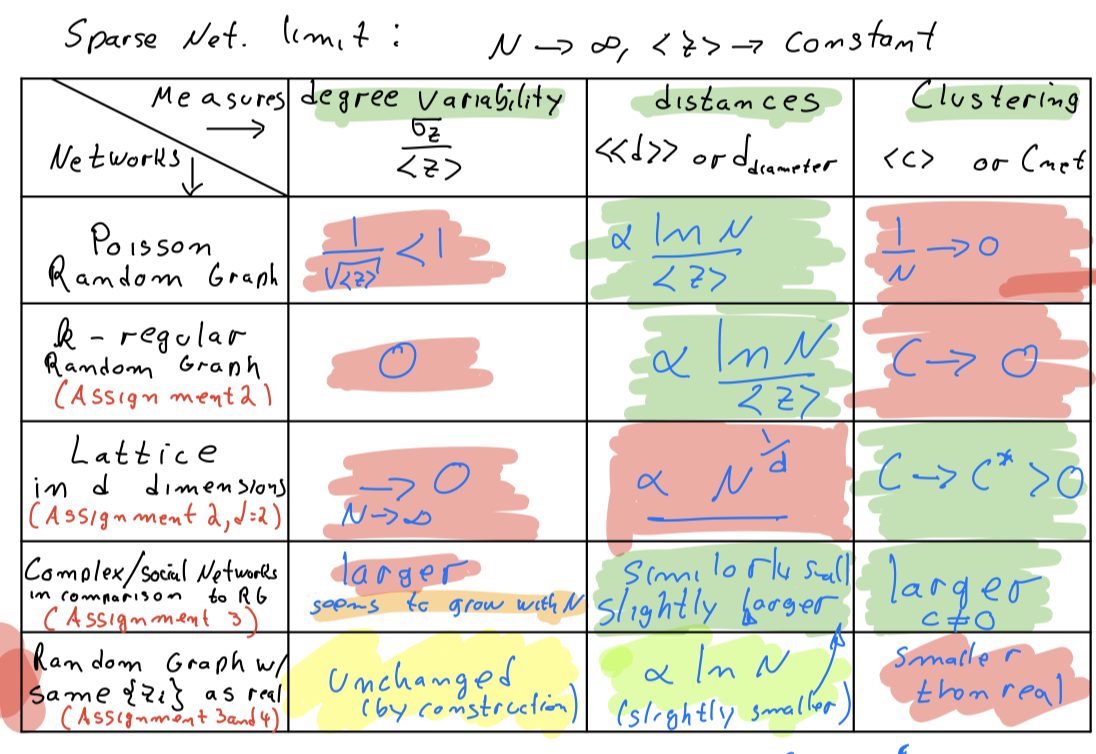
\includegraphics[scale=0.6]{Network-comparison}
\end{center}

We see 3 main conflicts between our empirical observations so far and the models we have looked at so far.
\begin{enumerate}
\item The random graph model correctly describes short distances $\langle \langle d \rangle \rangle \approx logN$ but underestimates the clustering $C \not \rightarrow C^* \neq 0$.
\item The Lattice models correctly describe the clustering coefficient $C  \rightarrow C^* \neq 0$ but fail at capturing short distances $\langle \langle d \rangle \rangle \neq log\;N$.
\item The degree variability seen in real networks are much larger than what our models account for. In fact, $\frac{\sigma_z^2}{\langle Z \rangle}$ grows with the number of nodes N.
\end{enumerate}

In particular, point 1 and 2 capture the \textbf{small world phenomena} of networks. Meanwhile, point 3 is known as the \textbf{scale-free} property of networks. 

We are interested in examining the degree variability of the network and how does it grow with N. We give a proposal on why is this the case.

\begin{definition_exam}{Fat Tail Degree Distribution}{} The degree distribution $P(Z)$ has a fat tail if the density is given by 
$$
P(Z = z) \approx z^{-\gamma}
$$
for $z >> 1.$
\end{definition_exam}

We are now interested in examining the moments of this fat tail degree distribution.

\begin{proposition_exam}{Second moment of scale-free networks diverges}{} The second moment diverges for a scale-free network for a scaling parameter $\gamma \leq 3.$
\end{proposition_exam}
\begin{proof}
For the scale-free property, the degree distribution is given by
$$
P(z) = \sum_{g \in \Omega}p(g)\delta (z(g) - z)
$$
has a fat tail whereby $P(Z) \sim Z^{-\gamma}$ for $Z >> 1.$ The second moment diverges as
$$
\langle Z^2 \rangle = \sum_{z=1}^{\infty}z^2P(Z = z) \approx \int_{1}^{\infty}z^2z^{-\gamma}dz \rightarrow \infty
$$
for $\gamma \leq 3.$
\end{proof}
\begin{remark} For $\gamma \geq 3,$ the network now looks like a Poisson random graph whereby the second moment is now finite and has a similar degree distribution.
\end{remark}

\begin{corollary}The degree fluctuation of the scale-free network diverges $$\sigma_Z = \sqrt{\langle Z^2 \rangle - \langle Z \rangle^2} \rightarrow \infty$$ as $N \rightarrow \infty.$
\end{corollary}

We have shown that the second moment diverges. Now, we are interested in seeing how does the second moment depend on the sample size N? We are interested in examining the second moment for a finite sample.

\begin{proposition_exam}{Second moment of finite sample}{} The second moment of the degree distribution for a finite sample in a power law network grows as a power of N 
$$
\langle Z^2 \rangle \approx \cdot N^{\beta}
$$
where $\beta = -1 + \frac{3}{\gamma}.$ Therefore, we have that the second moment grows linearly with N
$$
\langle Z^2 \rangle \propto N
$$
for $2 \leq \gamma \leq 3$.
\end{proposition_exam}

\begin{proof} First, we note that the maximum $Z = Z_{max}$ has probability of being observed 
$$
P(Z_{max}) = \frac{1}{N}
$$
and therefore from this, we can conclude that the second moment of the degree distribution for a finite sample is given by 
$$
\langle Z^2 \rangle \approx \sum_{Z=1}^{Z_{max}}Z^2p(z) \approx \int_{1}^{Z_{max}}c\cdot z^{-\gamma + 2}dz =  N^{\beta}
$$
where $\beta = -1 + \frac{3}{\gamma}.$ 
\end{proof}


Now, we will discuss more about scale-free networks.
\subsection{Scale-Free Networks}

Power law distributions come up in many different types of networks. Most real world networks have fat tails in their distribution of degrees for nodes. That is, we have alot of hubs in our networks that our random graph models are unable to account for. It is this diversity of scenarios in which the scale-free property appears that prompts us to call the scale-free property a universal network characteristic.

\begin{center}
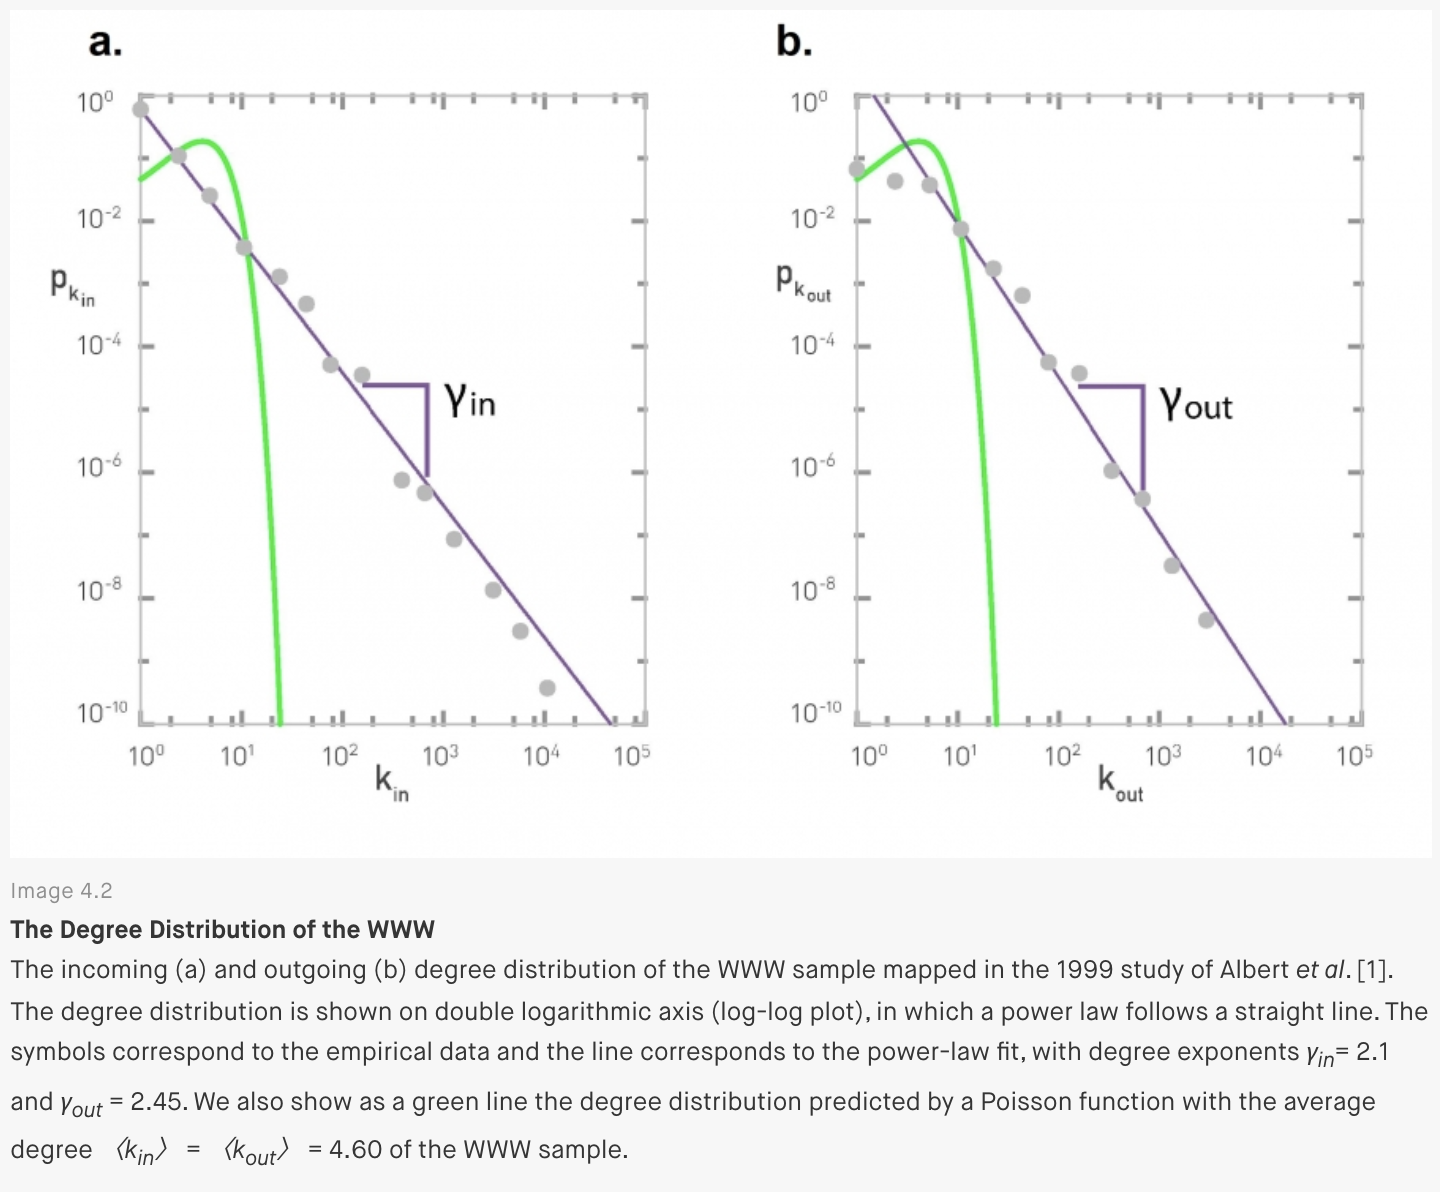
\includegraphics[scale=0.6]{WWW}
\end{center}

We can see that the scale-free network fits the degree distribution of the World Wide Web compared to the Poisson random graph.

\begin{definition_exam}{Power Law Distribution}{}Let $P(Z=z)$ be the probability that a node has degree z. Then, the \textbf{power law distribution} is given by 
$$
P(Z=z) \approx z^{-\gamma}
$$
where $\gamma$ is the degree exponent.
\end{definition_exam}

\begin{remark}Empirically, we usually have $2 \leq \gamma \leq 3$ for large z.
\end{remark}

If we take log transformations of both sides to get 
$$
log P(Z=z) \approx -\gamma log z
$$
then if we plot the empirical histogram of number of data points with their degree on a log-log plot, then it should be a straight line.

\begin{definition_exam}{Scale-Free Networks}{}A scale-free network is a network whose degree distribution follows a power law.
\end{definition_exam}

Now, revisiting our previous observation that many real-world networks have degree distributions with fat tails, there are 2 ways we can interpret this.

A weak interpretation is that the degree variability $\frac{\sigma_Z}{\langle Z \rangle} \rightarrow \infty$ as $N \rightarrow \infty$. This is weak in the sense that it only comments on the moments of the distribution.

A stronger interpretation is when we comment on the degree distribution itself. That is, we posit that the degree distribution follows a power law distribution 
$$
P(Z = z) \approx z^{-\gamma}
$$
for $2 \leq \gamma \leq 3$ for a large z.

Hence, we will move onto \textbf{mechanistic models} that account for these observations.



\subsection{Discrete and Continuum Formalism of Degree Distribution}
In this section, we give a rigorous derivation of the degree distribution for the power law in both the discrete and continuous case.

We first define how we can compute the probability that $P(Z=z)$ for $z \in \mathbb{N}$. First, we want to compute 
$$
P(Z=z) = Cz^{-\gamma}
$$
where C is determined by the normalization condition $\sum_{z=1}^{\infty}P(Z=z) = 1.$ Hence,
$$
C\sum_{z=1}^{\infty}z^{-\gamma} = 1.
$$
Solving for C, we get 
$$
C = \frac{1}{\sum_{z=1}^{\infty}z^{-\gamma}} = \frac{1}{\zeta (\gamma)}
$$
where $\zeta(\gamma)$ is the Riemann-Zeta function.

\begin{definition_exam}{Discrete Power-Law Distribution}{}For $z \in \mathbb{N}$, the discrete power law has the distribution 
$$
P(Z=z) = \frac{z^{-\gamma}}{\zeta(\gamma)} = \frac{z^{-\gamma}}{\sum_{z=1}^{\infty}z^{-\gamma}}
$$
\end{definition_exam}

\begin{remark}The discrete power law diverges for z = 0.
\end{remark}

We now look at the continuous formulation where $z \in \mathbb{R}^+.$ We define the probability density function as
$$
f(z) = Cz^{-\gamma}
$$
where the normalization condition is now 
$$
\int_{z_{min}}^{\infty}f(z)dz = 1
$$
where $z_{min}$ is the minimum degree in our degree distribution.

\begin{definition_exam}{Continuous Power-Law Distribution}{}For $z \in \mathbb{R}^+$, the continuous power law has the distribution 
$$
f(z) = (\gamma - 1)z_{min}^{\gamma - 1}z^{-\gamma}
$$
where $z_{min}$ is the smallest degree for which the power law holds.
\end{definition_exam}

\begin{remark}
Note that in the continuous formalisation, the definition above is actually the density function. We can only can talk about 
$$
\int_{z_{1}}^{z_{2}}f(z)dz
$$
which talks about the probability that a randomly chosen node has degree between $z_1$ and $z_2.$
\end{remark}

\subsection{Hubs in scale-free networks}
We contrast the differences between the scale-free networks and the Poisson random graph.
\begin{enumerate}
\item For a small degree z, the power law distribution is much greater than the Poisson distribution. This indicates that the network has many nodes with small degrees, a property that is seen in real networks.
\item For z in the vicinity of $\langle Z \rangle$, we see that the Poisson distribution is greater than the power law.
\item For a large degree z, we see that the power law distribution is greater than the Poisson distribution. This captures the hubs in the network.
\end{enumerate}

\begin{center}
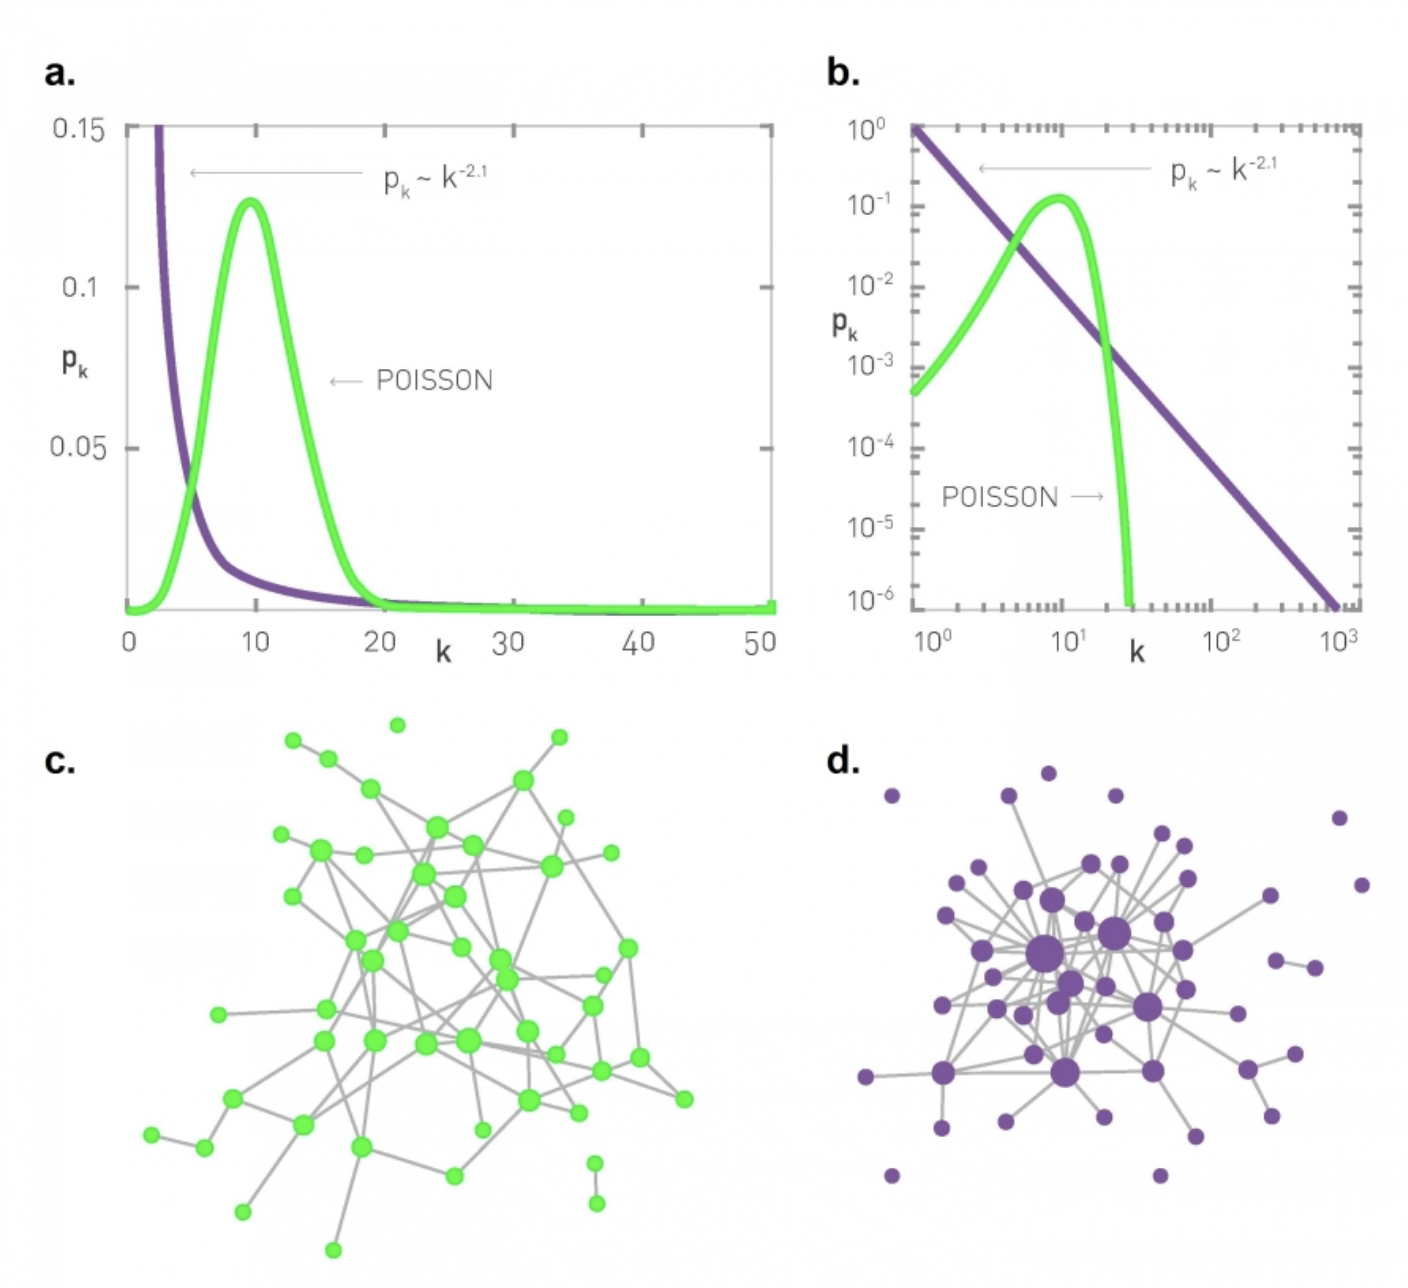
\includegraphics[scale=0.3]{Poisson-Scale-Free}
\end{center}

In alot of real world networks, the Poisson distribution would not have predicted hubs as it assigns the probability of a node with having a large number of numbers practically impossible. Hence, the Poisson random graph is not a good description of real world networks.

We will now contrast the growth of the size of hubs for scale-free networks and the exponential distribution.

A very important remark to make between the difference of a power law distribution and exponential distribution is that the exponential distribution is given by 
$$
P(x) \approx e^{-x}
$$
whilst a power law is given by 
$$
P(x) \approx x^{-\gamma}
$$
where we can see that the exponential distribution decays alot faster.

\begin{theorem}(Growth of maximum degree in exponential distribution). Let $z_{min}$ be the smallest degree observed in the network and $z_{max}$ be the largest degree. We have that the formula for the size of the largest hub in an exponential distribution is 
$$
z_{max} = z_{min} + \frac{ln N}{\gamma}.
$$
\end{theorem}

\begin{remark}The growth of $z_{max}$ in a random graph model hardly grows due to the ln N term. That is, we expect $z_{max} \approx z_{min}$.
\end{remark}
The Poisson random graph grows even more slowly than this.

\begin{theorem}(Growth of maximum degree in power law distribution). Let $z_{min}$ be the smallest degree observed in the network and $z_{max}$ be the largest degree. We have that the formula for the size of the largest hub in the power law distribution is 
$$
z_{max} = z_{min}N^{\frac{1}{\gamma - 1}}.
$$
\end{theorem}

\begin{remark}We see that the larger the network, the larger the degree of the biggest hub of the scale free network.
\end{remark}

In a random network most nodes have comparable degrees and hence hubs are forbidden. Hubs are not only tolerated, but are expected in scale-free networks. Furthermore, the more nodes a scale-free network has, the larger are its hubs. Indeed, the size of the hubs grows polynomially with network size, hence they can grow quite large in scalefree networks. In contrast in a random network the size of the largest node grows logarithmically or slower with N, implying that hubs will be tiny even in a very large random network.

We can contrast the growth of the degree of the largest degree node for a scale-free network vs a Poisson random graph.
\begin{center}
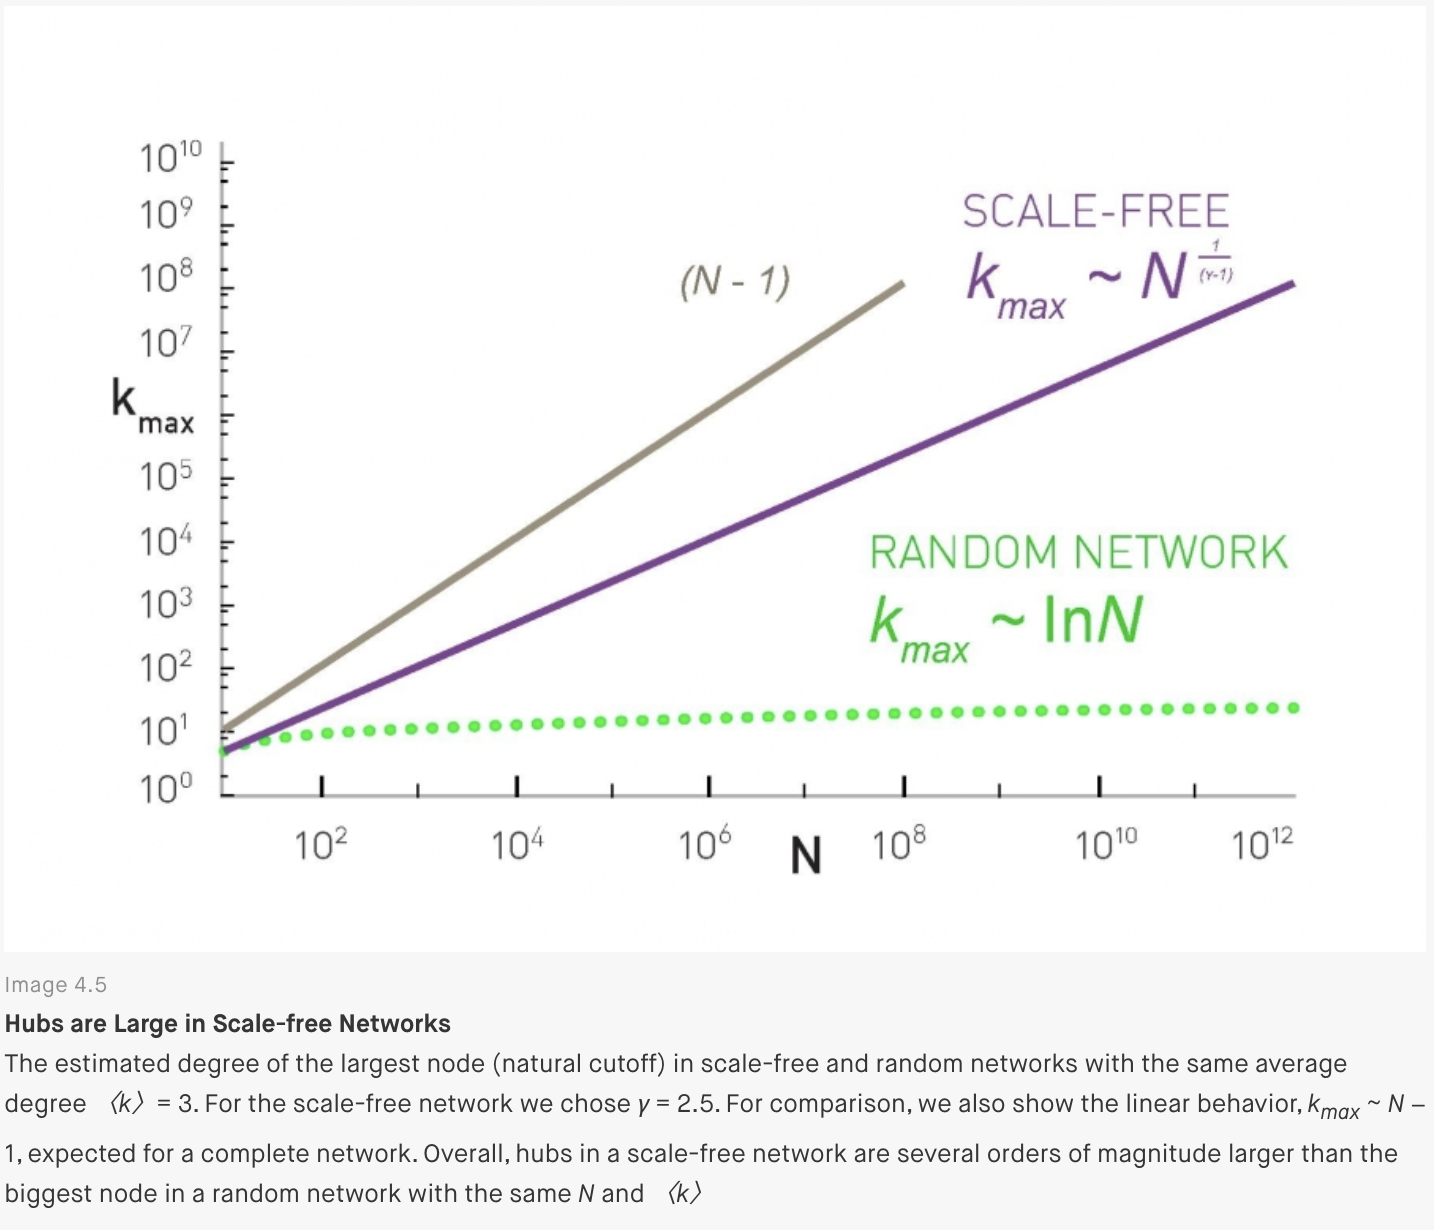
\includegraphics[scale=0.3]{Growth-hub}
\end{center}

\subsection{Scale-Free Property of Networks}

We now investigate what does the scale-free property mean. To best understand the meaning of the scale-free term, we need to familiarize ourselves with the moments of the degree distribution.

\begin{definition}(Moments). The $n^{th}$ moment of the degree distribution is defined as 
$$
\langle Z^n \rangle = \int_{z_{min}}^{\infty}z^nf(z)dz,
$$
\end{definition}

\begin{proposition_exam}{Moments of Scale-free network}{}For a scale-free network, the $n^{th}$ moment of the degree distribution is given by 
$$
\langle Z^n \rangle = \int_{z_{min}}^{z_{max}}z^nf(k)dk = C\frac{z_{max}^{n - \gamma + 1} - k_{min}^{n - \gamma + 1}}{n - \gamma + 1}.
$$
\end{proposition_exam}

\begin{remark}Recall that $z_{min}$ is usually fixed whilst the degree of the largest hub $z_{max}$ increases with the size of the system.
\end{remark}

The limit of $\langle Z^n \rangle$ depends on $\gamma$ and n, where n is the moment we are looking at. Note that only $k_{max}$ is the term that increases in our equation above.

\begin{proposition_exam}{Behaviour of moments in power law networks}{} Let $\langle Z^n \rangle$ be the $n^{th}$-moment of the distribution of node degrees in the network. Let $\gamma$ be the degree exponent of the power law. Let $z_{max}$ be the degree of the largest hub. Then, we have the following:
\begin{enumerate}
\item If $n - \gamma + 1 \leq 0$, then all the $n^{th}$-moments for which this holds $\langle Z^n \rangle$ are finite as $z_{max} \rightarrow \infty.$
\item If $n - \gamma + 1 > 0$, then all moments $\langle Z^n \rangle \rightarrow \infty$ as $z_{max} \rightarrow \infty.$ 
\end{enumerate}
\end{proposition_exam}

For many scale-free networks, the degree exponent $\gamma \in [2,3].$ Then, in scale-free networks, we have that the first moment $\langle z \rangle$ is finite but higher moments $\langle Z^n \rangle$ go to infinity.

\begin{center}
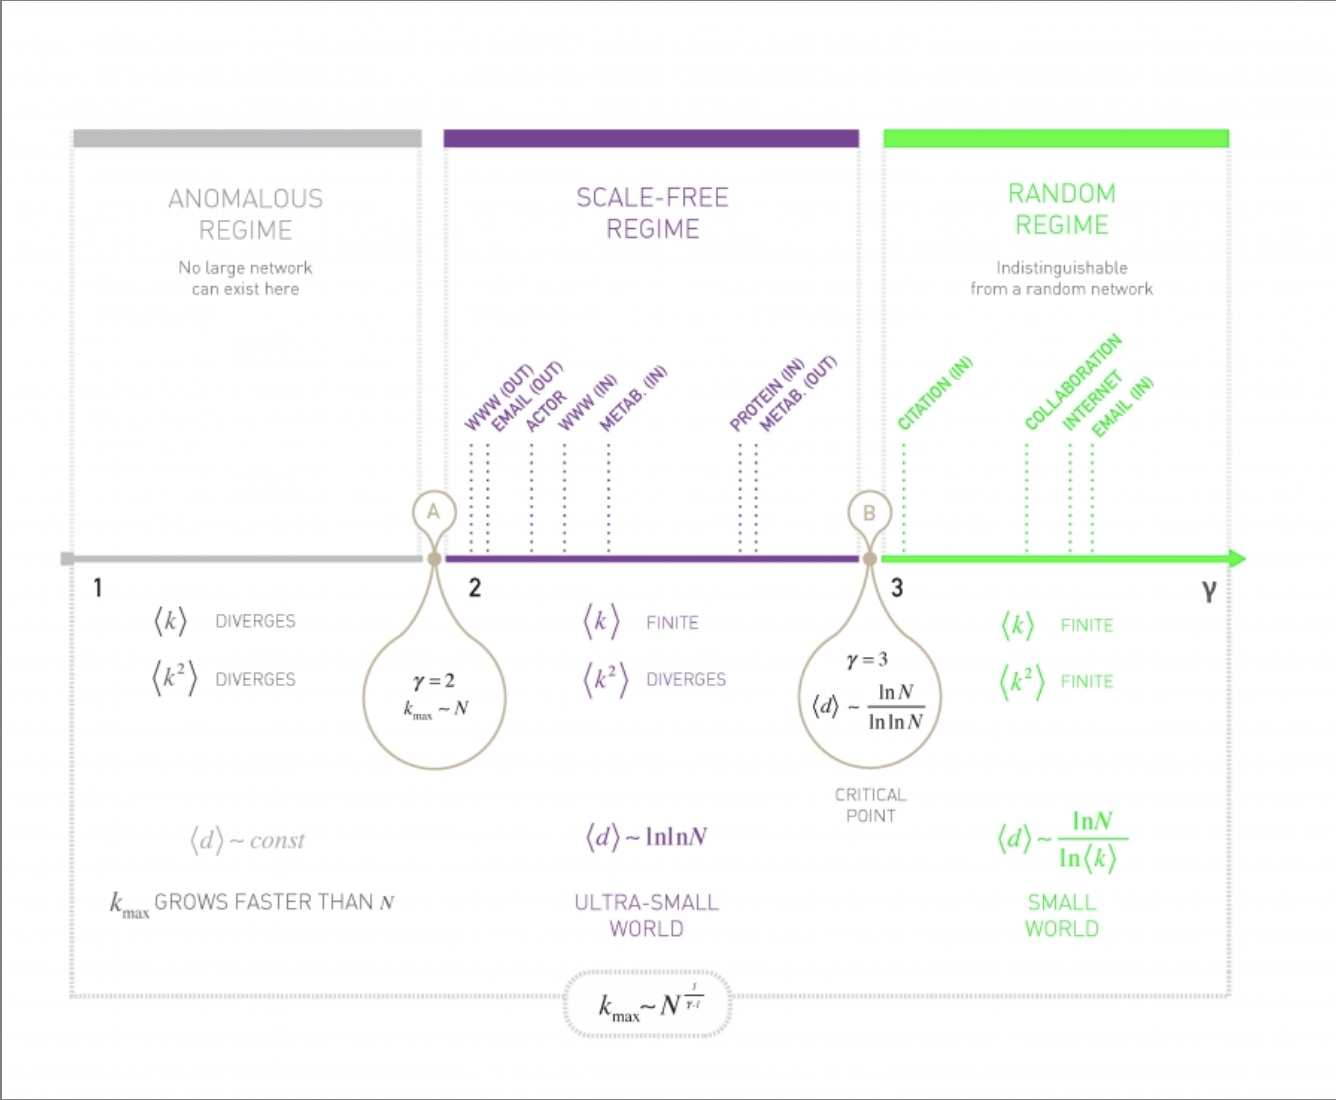
\includegraphics[scale=0.4]{Scale-free-regimes}
\end{center}

Therefore, it is important to note that scale-free networks only exist between the range $2 \leq \gamma \leq 3.$ If $\gamma \geq 3,$ then the network looks like a random graph as the second moment is now defined. If $\gamma \leq 2,$ then no large network can exist as for sufficiently large N, the degree of the largest hub of the network exceeds the total number of nodes in the network, which does not make sense.


\textbf{Random networks such as the Poisson random graph has scale. By that, the nodes in the Poisson random graph will have comparable degrees and hover around the first moment $\langle z \rangle.$}

\textbf{Scale-free networks lack a scale. If $\gamma < 3$, the first moment is finite but higher moments are infinite. Then, we have that $\langle Z^2 \rangle$ and $\sigma_z$ diverges for a large number of nodes N.} \textbf{What this means is that for a scale-free network, when we randomly choose a node, we do not know what to expect. The fluctuations around the average $\langle z \rangle$ can be arbitrarily large.} 

Scale-free networks has some interesting properties with regards to network distances. 
\begin{enumerate}
\item Scale-free networks shrink the average path lengths. Hence, we have "ultra-small" world.
\item The smaller $\gamma$ is, the shorter are the distances between the nodes.
\item Hubs decreases the average path lengths in the network.
\end{enumerate}

\subsection{Barabási-Albert Model}

It is interesting to note that such a wide range of networks have the scale-free property. Hence, in order for such different systems to converge to a similar architecture, it is likely that the mechanism for the explanation is a simple and fundamental one. Hence, we move away from describing a network's topology to \textbf{modeling the evolution of a complex network}. We now describe the generative process for constructing scale-free networks. Consequently, the modeling philosophy behind the model is simple: to understand the topology of a complex system, we need to describe how it came into being.

There are 2 explanations for why a random network differs to real networks.
\begin{enumerate}
\item \textbf{Growth}: Real networks are a result of a growth process which grows over times as more nodes gets added to the system.
\item \textbf{Preferential Attachment}: New nodes are more likely to connect to more connected nodes.
\end{enumerate}

We begin our set up with $N_0$ nodes with links distributed arbitrarily.
\begin{definition}(Growth). At each timestep, we add a new node with $m \leq N_0$ links that connects the new node to m existing nodes.
\end{definition}


\begin{definition}(Preferential Attachment). We define the probability $\pi_i(z_i)$ that a link of the new node connects to node i depends on the degree $z_i$ as 
$$
\pi(z_i) = \frac{z_i}{\sum_{i=j}^{N(t)}z_j} = \frac{z_i}{2L(t)}
$$
where L(t) is the number of links in the network at time t and $N(t)$ is the number of nodes at time t.
\end{definition}

We now note that in fact, these 2 factors are extremely important.
\begin{theorem_exam}{Necessary and sufficient conditions for scale-free networks}{} The combination of both growth and preferential attachment are necessary and sufficient conditions to generate a network that is scale-free.
\end{theorem_exam}

\begin{theorem_exam}{Barabási-Albert Model}{}Let our network start off with $N_0$ nodes with links distributed across these nodes. The Barabási-Albert model has two steps:
\begin{enumerate}
\item \textbf{Growth}: At every time step, we add a new node with m links to add.
\item \textbf{Preferential attachment}: With our new node, we have a probability of our node to add a link to node i with probability $\pi_i(z_i) = \frac{z_i}{\sum_{i=j}^{N(t)}z_j}$ at time t.
\end{enumerate}
\end{theorem_exam}

We are now interested in the asymptotics of the Barabási-Albert model.

\begin{proposition_exam}{Asymptotics of Barabási-Albert Model}{}Let our network start off with $N_0$ nodes. Then, after t timesteps, the Barabási-Albert model generates a network with
\begin{enumerate}
\item $N = N_0 + t \approx t$ nodes for $N_0 << N$
\item $L = L_0 + m\cdot t \approx m\cdot t$ links for $L_0 << L$
\item $\sum_{i=1}^{N}z_i = 2L \approx 2m\cdot t$ as $t \rightarrow \infty$
\end{enumerate}
\end{proposition_exam}

\subsection{Degree Dynamics of Barabási-Albert Model}
We want to understand how does the scale-free property emerge. So first, we look at how does the degree of a node evolve over time. 

The main intuition we will use is that an existing node can potentially increase its degree each time a new node enter the network. 

We will focus on a node i with that was created at time $0 \leq t_i \leq t$ with degree $z_i(t).$ Here, we have that $z_i >> 1, t >> 1$ and $t_i << t.$ That is, we examine a node that has been created a long time ago and we now analyse how its degree has changed over time.

\begin{theorem_exam}{Growth of the degree of a node}{} Suppose that node i was created at time $t_i$. Then, the degree of a node i grows with $\sqrt{t}$, that is 
$$
z_i(t) = m \sqrt{\frac{t}{t_i}}
$$
for a given time point $t >> t_i$.
\end{theorem_exam}

\begin{proof} We use a continuous approximation of the node i's degree. First, we have that 
$$
\frac{dz_i}{dt} = m \pi_i(z_i(t)) = \frac{mz_i}{2L} \approx \frac{z_i}{2t}
$$
since $L \approx mt$ as $t \rightarrow \infty.$ Then, we can solve the 1st order ODE 
$$
\frac{1}{z_i}dz_i = \frac{1}{2t}dt
$$
to arrive at 
$$
z_i = A\sqrt{t}
$$
where $A = e^c.$ From this, we know that the initial condition of node i being created at time $t_i$ had m edges 
$$
z_i(t = t_i) = m
$$
and from this, we can deduce that 
$$
z_i(t) = m \sqrt{\frac{t}{t_i}}
$$
\end{proof}

\begin{remark} The significance of this result is that the degree of a node grows over time. That is, it is the rich gets richer phenomena. Therefore, the older the node, the higher its degree.
\end{remark}


With this, we can state an interesting phenomena.

\begin{lemma}(Rich-gets-richer phenomena). Larger nodes are more likely to acquire more links at the expense of smaller nodes due to preferential attachment.
\end{lemma}


We now know the evolution of a given node's degree. We wish to derive the distribution of degrees of the network in general. To do this, we first derive the cumulative distribution function of the degree distributions and from that, derive the density function. 

We are interested in the cumulative probability of a node i having a degree of a certain size 
\begin{equation}
\prob(Z_i(t) > z) = \prob(t_i > \frac{m^2t}{z^2})
\tag{*}
\end{equation}
where we used the fact that $z_i(t) = m \sqrt{\frac{t}{t_i}}$. Before we proceed, we recall something else. First, we examine the probability of a node being created at time $t_i.$ In particular, the probability of a node being created at time step $t_i$ is equiprobable and hence 
\begin{equation}
\prob(t_i) = \frac{1}{N} \approx \frac{1}{N_0 + t} \approx \frac{1}{t}
\tag{**}
\end{equation}

Now, going back to (*) and using the result (**) we can conclude that 
$$
\prob(t_i > \frac{m^2t}{z^2}) = 1 - \prob(t_i < \frac{m^2t}{z^2}) = 1 - \frac{m^2t}{z^2}\frac{1}{N} \approx 1 - \frac{m^2}{z^2}
$$

Therefore, we now have the cumulative distribution function of the degree of the network 
$$
\prob(Z_i < z) \approx \frac{m^2}{z^2}
$$
and we can take the derivative of this to get the density function.

\begin{proposition_exam}{Density of the degree of the network under the Barabási-Albert Model}{} The density function of the degree distribution of the network generated by the Barabási-Albert model is 
$$
p(z) = \frac{\partial}{\partial z}\prob(Z < z) \approx \frac{1}{z^3}
$$
\end{proposition_exam}


\begin{remark} We therefore have that the degree distribution of the network under the Barabási-Albert model generates a power law distribution!
\end{remark}


\begin{remark}We require both the presence of growth and preferential attachment if we want the power law degree distribution to emerge.
\end{remark}

We now state the clustering coefficient and diameter of the Barabási-Albert model.
\begin{proposition_exam}{Clustering coefficient of Barabási-Albert Model}{}The clustering coefficient of the Barabási-Albert model is given by 
$$
C \sim \frac{ln(N)^2}{N}
$$
\end{proposition_exam}
\begin{remark} The issue is that the clustering coefficient $C \rightarrow 0$ as $N \rightarrow \infty.$ However, it decays to 0 slower compared to the Poisson random graph model.
\end{remark}

\begin{proposition_exam}{Diameter of Barabási-Albert Model}{}The network diameter of the Barabási-Albert model is given by 
$$
d_{diam} \approx \frac{ln N}{ln (ln N)}
$$
\end{proposition_exam}
\begin{remark}The Barabási-Albert model grows at the same rate as actual random networks but at a wrong constant.
\end{remark}

We now state what are the nice properties of the Barabási-Albert model.

\begin{proposition_exam}{Nice properties of the Barabási-Albert model}{}The networks generated under the Barabási-Albert model has the nice properties of 
\begin{enumerate}
\item The network is a simple graph 
\item The network is fully connected 
\item The network exhibits the power-law degree distribution
\end{enumerate}
\end{proposition_exam}

We now state some issues with the Barabási-Albert model.
\begin{proposition_exam}{Issues with the Barabási-Albert model}{}The networks generated under the Barabási-Albert model has the issues of 
\begin{enumerate}
\item It only generated a power law distribution with exponent $\gamma = 3$
\item The older nodes in the network are always hubs
\item The clustering coefficient goes to 0 $C \sim \frac{1}{N^{\beta}} \rightarrow 0$ for $\beta < 1$ as $N \rightarrow \infty$
\item There are power law distributions in under quantities such as the betweeness centrality which is not exhibited in the Barabási-Albert model
\end{enumerate}
\end{proposition_exam}



We now note a very important property of the power law distribution.

\begin{theorem_exam}{Scale Invariance of Power Law Distribution}{} The Barabási-Albert model generates a scale-free distribution. It is invariant under scaling. If 
$$
p(z) = c\cdot z^{-\gamma}
$$
then scaling it by a constant $\alpha$ gives us
$$
p(\alpha \cdot z) \approx p(z)
$$
\end{theorem_exam}
\begin{proof} Suppose that 
$$
p(z) = c\cdot z^{-\gamma}
$$
Then, we have that 
$$
p(\alpha \cdot z) = c(\alpha \cdot z)^{-\gamma} = c \alpha^{-\gamma}z^{-\gamma} = \alpha^{-\gamma}p(z) \approx p(z)
$$
as $\alpha^{-\gamma}$ is a constant.
\end{proof}

\begin{remark} This means that we have the same distribution after scaling. This is a fractal-like property.
\end{remark}



\lecture{10}{Watts-Strogatz Model}
\section{Scale-Free Networks}
\subsection{Watts-Strogatz Model}


We have previously explored the degree variability of networks. Now, recall two other observations we noted in real world networks.
\begin{enumerate}
\item \textbf{Short distances in networks}: The average distance between 2 nodes depends logarithmically on N.
\item \textbf{High Clustering}: The average clustering coefficient of real networks is much higher than that expected of a random network.
\end{enumerate}

Having only small distances in a network is not surprising as this is common in random network. It is simultaneously having both small distance and high clustering in a network that is unusual. Recall that for Poisson random graphs, we derived that the diameter was given by 
$$
d_{max} \approx \frac{ln N}{ln \langle Z \rangle} \approx ln(N)
$$
in the sparse limit. However, we showed as well that the clustering coefficient goes to 0 in the Poisson random graph 
$$
C = q = \frac{\langle Z \rangle}{N} \rightarrow 0
$$
Therefore, we need to find a way to explain both properties observed in networks. We give this anomaly a proper name.

\begin{definition_exam}{Small World Property}{} The small world property is when in an observed network, the average distance between two nodes is small but the clustering coefficient is large.
\end{definition_exam}

The Watts-Strogatz model builds off the idea of the small world property. The Watts-Strogatz model is an interpolation between a regular lattice (high clustering but large distances) and random network (small clustering but small distances).


\begin{theorem_exam}{Watts-Strogatz Model}{} The Watts-Strogatz comprises of two steps
\begin{enumerate}
\item Start with a ring where each of the node is connected to Q neighbours based on ring distance.
\item For each of the L links, we rewire the link with probability p. That is, we can either
\begin{enumerate}
\item Delete the link and add a new random link 
\item Delete one end of the link and attach it randomly to a new node
\end{enumerate}
\end{enumerate}
\end{theorem_exam}

\begin{remark} This form of rewiring the network preserves the number of links in the graph and hence the network has a well-defined network limit. The probability p can be thought of as a parameter to the model.
\end{remark}

\begin{remark}Clearly, we require the number of neighbours $Q << N.$
\end{remark}

The interest now is looking at how does varying the probability of rewiring (p) affect the network's topology. In particular, we want to focus on the clustering C and average distance $\langle \langle d \rangle \rangle.$


First, we look at the extreme end for when we do not do any rewiring of the ring $p = 0.$

\begin{proposition_exam}{Watts-Strogatz model with no rewiring}{} Suppose we have a Watts-Strogatz model where each node is connected to its Q nearest neighbours. Suppose we do not rewire any links i.e. p = 0. Then, we have the following properties of the network. 
\begin{enumerate}
\item The network will be sparse 
$$
L = Q \cdot N
$$
\item The network will exhibit high clustering 
$$
C_{ring} \approx \frac{3}{4}
$$
\item The network \textbf{does not} exhibit small distances 
$$
\langle \langle d \rangle \rangle \approx N
$$
\end{enumerate}
\end{proposition_exam}

\begin{proof} First, to show that the network is sparse, we have that 
$$
L = \frac{\langle Z \rangle N}{2} = Q \cdot N
$$
Now, to show the average clustering, as each node has the same number of neighbours, the average clustering is the clustering of a given node. 
$$
\langle C \rangle = C_i = \frac{\# \text{ of triangles}}{Z_i(Z_i - 1)} = \frac{3Q(Q - 1)}{2Q(2Q - 1)} = \frac{3Q - 1}{4Q - 1} \approx \frac{3}{4}
$$
since we have that $Z_i = 2Q$ and the number of triangles is $3 {Q \choose 2} = \frac{3Q(Q - 1)}{2}.$ 

Finally, the network diameter is given by 
$$
d_{diam} = \frac{N}{2Q}
$$
as we can walk in steps of size Q. From this, we have that 
$$
\langle \langle d \rangle \rangle \approx \frac{d_{diam}}{2} \propto N
$$
\end{proof}

We now look at the other extreme end of rewiring.

\begin{proposition_exam}{Watts-Strogatz model with complete rewiring}{} Suppose we have a Watts-Strogatz model where each node is connected to its Q nearest neighbours. Suppose we rewire all links i.e. p = 1. Then, we have the following properties of the network. 
\begin{enumerate}
\item The network will be sparse
\item The network will exhibit no clustering 
$$
C_{RG} \approx 0
$$
\item The network \textbf{does} exhibit small distances 
$$
\langle \langle d \rangle \rangle \approx log(N)
$$
\end{enumerate}
\end{proposition_exam}
\begin{proof} This automatically follows as for $p \rightarrow 1,$ the graph becomes a Poisson random graph.
\end{proof}

Now, in between these two extremes, we can look at the interpolation between the two types of graphs. We will soon see that there exists a range of p for which the small world property arises. We now examine the behaviour of increasing the probability of a link rewiring on the ring network.
\begin{proposition_exam}{Clustering coefficient as we vary probability of rewiring}{} Let p be the probability of rewiring a link in the network. Then, we have that the clustering coefficient of the network for a graph with rewiring probability $p > 0$ as 
$$
C \approx \frac{3}{4}(1 - p)^3
$$
\end{proposition_exam}

\begin{proof}  Let $C_{ring}$ be the clustering coefficient of the ring network with p = 0. First, note that 
$$
C = C_{ring}(1 - p)^3
$$
where the probability of each of the link in a triangle not being rewired and broken is given by $(1 - p)^3.$ As shown earlier, $C_{ring} \approx \frac{3}{4}.$
\end{proof}
\begin{corollary} As the rewiring probability $p \rightarrow 1,$ the clustering coefficient gets smaller.
\end{corollary}
\newpage
We now want to look at how does varying the rewiring probability p affect the distance d of the network. First, it is important to note that every link that is rewired creates a shortcut that connects a region far from the node. Therefore, we have that the distance d decays as soon as the number of shortcuts are significant, that is, it is larger than a given number A.

\begin{proposition_exam}{Number of shortcuts in a network}{} The number of shortcuts in the network with rewiring links is given by 
$$
\text{\# shortcuts} = p\cdot Q\cdot N  > A
$$
for a constant A where $Q \cdot N$ is the number of links in the network L and Q is the number of neighbours a node is connected to.
\end{proposition_exam}

\begin{corollary}The rewiring probability for the number of shortcuts in the network to be significant is given by 
$$
p > p^* = \frac{A}{Q\cdot N} \rightarrow 0
$$
as $N \rightarrow \infty.$
\end{corollary}

\begin{remark} The percolation threshold $p^*$ gets smaller as the number of nodes and therefore links in the network increases. The effect of rewiring has a quick effect of decreasing the distance in the network.
\end{remark}

From these discussions, we come to our important result in the Watts-Strogatz model.
\begin{theorem_exam}{Small world regimes in Watts-Strogatz model}{} For a range of probabilities of rewiring links p, there is a region in which networks exhibit small world properties. That is, they will have high clustering coefficients yet have short distances in the network.
\end{theorem_exam}

\begin{center}
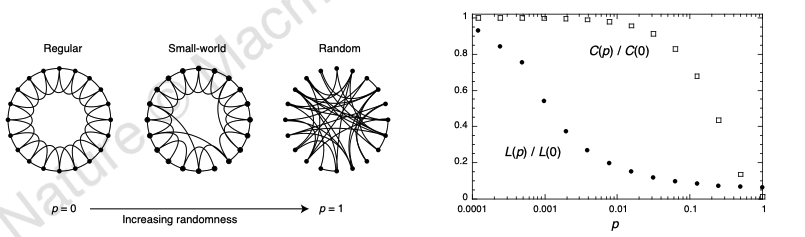
\includegraphics[scale=0.6]{Small-world}
\end{center}

We come to the big takeaway of this section to explain the appearance of small world properties in networks. If we start off with a lattice, simply rewiring a few links will dramatically cut the distance of the network yet maintain the high clustering coefficient of the network. There is a nonlinear effect of the probability of rewiring on the distances found in the network whilst the probability of rewiring has a linear effect on the clustering.

However, the problem with the Watts-Strogatz model is that it does not exhibit variation in its degree distribution. This is because we fixed the number of nodes to begin with. Therefore, the degree distribution looks similar to that for the Poisson random graph and regular lattice.

\begin{center}
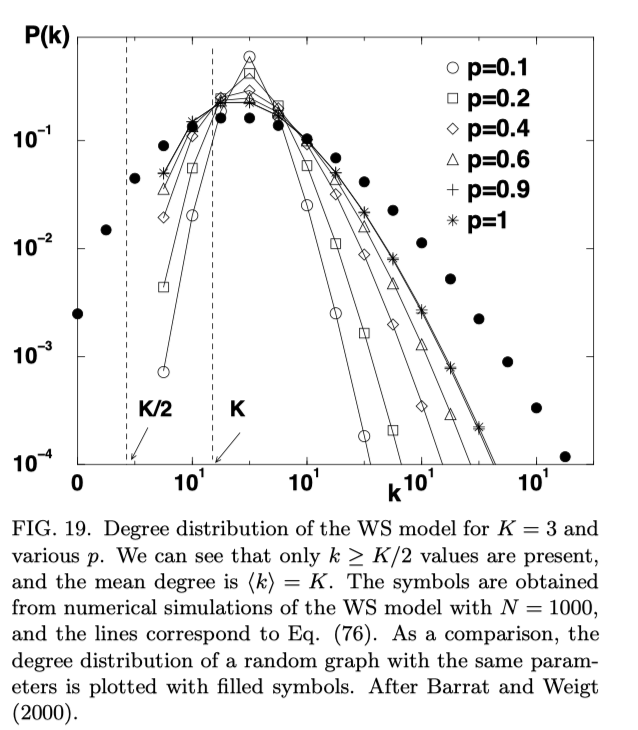
\includegraphics[scale=0.7]{Watts-Strogatz}
\end{center}

\lecture{11}{Percolation Theory}
\section{Network Robustness}
\section{Network Robustness}
\subsection{Percolation Theory}
We are interested in how sensitive are networks against pertubations. We describe the set up of the problem.

\begin{enumerate}
\item Start off with a network
\item Delete a fraction "q" of nodes or links 
\item We measure how a network property x depends on the fraction q deleted
\end{enumerate}

In order to solve this, we first look at Percolation theory. Percolation theory is a highly developed subfield of statistical physics and mathematics.

First, for each link/node, we define a state variable where
$$
\phi_i = 
\begin{cases}
1 \quad \text{on or occupied}\\
0 \quad \text{off or empty}\\
\end{cases}
$$

In terms of assigning states to nodes in the network, we can choose $\phi_i$ for each node i such that 
$$
\langle \phi_i \rangle = \frac{1}{N}\sum_{i=1}^{N}\phi_i = p
$$
where p is the fraction of nodes in the network being on. Alternatively, we can interpret p as the probability for a node i to be on. Additionally, we define 
$$
q = 1 - p
$$
to be the probability that a node is off.

The main question in percolation theory is what is the probability $\pi$ that there is a connected path between the 2 sides of the network?

\begin{proposition_exam}{Percolation transition}{}Let $\pi$ be the probability that there is a connected path between the 2 sides of the network. Then, as $N \rightarrow \infty$
$$
\pi =
\begin{cases}
0 \quad \text{if } p < P_c\\
1 \quad \text{if } p > P_c
\end{cases}
$$
where P is the fraction of nodes we don't delete from the network and $P_c$ is the \textbf{percolation transition threshold}.
\end{proposition_exam}

\begin{example}(Percolation threshold in the 1D Lattice). The percolation threshold $P_c = 1$ in the 1D-lattice.
\end{example}

\begin{example}(Percolation threshold in the 2D Lattice). The percolation threshold $P_c$ in the 2D-lattice is 
$$
P_c = 0.5.
$$
\end{example}

\begin{proof} First, recall that the degree distribution of the Bethe lattice is given by 
$$
P(Z) = \delta (Z - 3)
$$
where each node has a degree of 3 and the Bethe lattice is itself a tree. We then ask what is the probability $\theta(p)$ that we can travel an arbitrarily long distance in the Bethe lattice if the probability of a node being on is p. First, we define the complement as 
$$
\omega = 1 - \theta
$$
Then, we see that there are 2 cases at which we stop travelling 
\begin{enumerate}
\item The link is off with probability $1 - p$
\item The link is on but leads to a dead end with probability $p \cdot \omega$
\end{enumerate}
Therefore, the probability for stopping for each link is $1 - p + p\cdot \omega.$ However, for each node, there are 2 outgoing links in the Bethe lattice and hence the probability of stopping is given by the self-consistency equation 
$$
\omega = (1 - p + p\cdot \omega)^2
$$
The solutions of this quadratic equation is 1 and $(\frac{1}{p} - 1)^2.$ Hence, using the fact that $\theta = 1 - \omega,$ the non-trivial probability of travelling arbitrary distances is given by 
$$
\theta = 0.5.
$$
\end{proof}

We keep these ideas of percolation theory in mind as we analyse network robustness.

\subsection{Molloy-Reed Criterion}

We are now interested in computing the percolation threshold for a random graph with a fixed degree distribution. For a network to have a giant component, most nodes that belong to it must be connected to at least two other nodes. This is captured in the Molloy-Reed criterion.
\begin{definition_exam}{Molloy-Reed Criterion}{}A random network will have a giant connected component if 
$$
\frac{\langle Z^2 \rangle}{\langle Z \rangle} \geq 2
$$
where Z is the degree distribution of the network.
\end{definition_exam}

\begin{proof} Recall that percolation occurs when we have one giant connected component. This occurs when we have that for a node i that is connected to node j, we also have one additional link. This is captured in 
$$
\langle z_i| i \leftrightarrow j \rangle \geq 2
$$
where $i \leftrightarrow j$ denotes that node i has a link with node j. This conditional probability allows us to determine the conditional expectation of the degree of node i 
\begin{equation}
\langle Z_i \rangle = \sum_{z=1}^{\infty}zP(Z=z|i \leftrightarrow j) \geq 2
\tag{*}
\end{equation}
Now, we note that in equation (*), we can apply Bayes theorem
$$
P(Z=z|i \leftrightarrow j) = \frac{P(z, i \leftrightarrow j)}{P(i \leftrightarrow j)} = P(i \leftrightarrow j|z)\frac{P(z)}{P(i \leftrightarrow j)}
$$
Now, we note that by random graph approximations, where we assume that the network is simple and has i.i.d edges, we have that 
$$
P(i \leftrightarrow j) = \frac{2L}{N(N - 1)} = \frac{\langle Z \rangle}{N - 1} \quad \text{and} \quad P(i \leftrightarrow j| z) = \frac{z}{N - 1}
$$
which express the fact that we can choose between N - 1 nodes to link to. Therefore, we conclude that in equation (*)
$$
\sum_{z=1}^{\infty}z\frac{z}{N - 1}\frac{P(Z=z)}{\frac{\langle Z \rangle}{N - 1}} = \sum_{z=1}^{\infty}\frac{z^2P(Z = z)}{\langle Z \rangle} = \frac{\langle Z^2 \rangle}{\langle Z \rangle} \geq 2
$$
\end{proof}

Hence, if a graph satisfies the Molloy-Reed criterion, we will have a giant connected component and hence we will be above the percolation threshold. We can apply this to the Poisson random graph.

\begin{proposition_exam}{Poisson Random Graph and connected component}{} The Poisson random graph with an average degree $\langle Z \rangle \geq 1$ satisfies the Molloy-Reed criterion and hence will have a giant connected component.
\end{proposition_exam}

\begin{proof} First, recall that 
$$
\langle Z^2 \rangle - \langle Z \rangle^2 = \langle Z \rangle
$$
as $\sigma_Z^2 = \langle Z \rangle.$ Therefore, we have that 
$$
\frac{\langle Z^2 \rangle}{\langle Z \rangle} = 1 + \langle Z \rangle \geq 2
$$
Therefore, we require that in order for the Molloy-Reed criterion to be satisfied, we need that $\langle Z \rangle \geq 1.$
\end{proof}

\begin{remark} We derive this same result when computing the transition threshold needed for a giant component to appear in a Poisson random graph!
\end{remark}

\subsection{Random Deletion of links}

We now go back to seeing how does pertubing the network affects it. In particular, we are interested in deleting the links of the network and seeing how does that affect the largest connected component.


\begin{lemma}(Degree distribution after link deletion). Let us have a random graph with degree distribution P(Z). We will delete links with probability $q = 1 - p$ and define $Z \rightarrow Z'$ as the change in degree distribution as a result of link deletion. Then the degree distribution with random deletion of links is given by
$$
P(Z') = \sum_{Z = Z'}^{\infty}P(Z)P(Z \rightarrow Z')
$$
\end{lemma}

\begin{proof} Note that as we delete links 
$$
z_i^{'} < z_i
$$
where $z_i^{'}$ is the degree of a node after links were deleted and $z_i$ was the degree of the node before links we deleted.
\end{proof}

Assuming our graph is a random graph we can compute the percolation transition threshold.

\begin{proposition_exam}{Critical threshold of a Random Graph}{}The Critical  threshold $q_c$ of a random graph is 
$$
q_c = 1 - \frac{1}{\frac{\langle Z^2 \rangle}{\langle Z \rangle} - 1}
$$
Therefore, if the fraction of links we delete from the network q is greater than $q_c$, then the network will not have a giant connected component.
\end{proposition_exam}

\begin{proof} First, we can use a Binomial distribution to model the new degree distribution 
$$
P(Z \rightarrow Z^{'}) = {Z \choose Z^{'}}(1 - q)^{Z^{'}}q^{Z - Z^{'}}
$$
Furthermore, we have that the first and second moments of this new degree distribution is 
$$
\langle Z^{'} \rangle = (1 - q)\langle Z \rangle \quad \quad \langle Z^{'\;2} \rangle = (1 - q)^2\langle Z^2 \rangle + q(1 - q)\langle Z \rangle
$$
using the fact that $P(Z \rightarrow Z^{'})$ is a Binomial distribution. Then, inserting these moments in the Molloy-Reed criterion, we get 
$$
\frac{\langle Z^2 \rangle}{\langle Z \rangle} = \frac{(1 - q)^2\langle Z^2 \rangle + q(1 - q)\langle Z \rangle}{(1 - q)\langle Z \rangle} = (1 - q)\frac{\langle Z^2 \rangle}{\langle Z \rangle} + q \geq 2
$$
By further algebra, we can then arrive at 
$$
q \leq 1 - \frac{1}{\frac{\langle Z^2 \rangle}{\langle Z \rangle} - 1} = q_c
$$
\end{proof}

\begin{remark} This is an interesting result as it only depends on the first and second moment of the original degree distribution!
\end{remark}

We can apply this to the Poisson random graph.
\begin{theorem_exam}{Critical Threshold of Poisson Random Graph}{} The critical  threshold of the Poisson random graph is 
$$
q_c = 1 - \frac{1}{\langle Z \rangle}
$$
\end{theorem_exam}

\begin{remark} This gives us the interesting insight that for the Poisson random graph, the denser the network, the higher its percolation transition threshold. This matches our intuition since there are alot more edges holding the network together.
\end{remark}

Now note that for a scale-free network, the degree distribution was given by $P(Z) \sim Z^{-\gamma}$ for $2 \leq \gamma \leq 3.$ Then, recall that the second moment diverges $\langle Z^2 \rangle \rightarrow \infty$ as $N \rightarrow \infty$. This means that the percolation transition threshold for the scale-free network is close to 1, that is, we need to delete alot of edges from the network before we can disconnect the network. 

\begin{proposition_exam}{Percolation Transition of Scale-Free Network}{}The percolation threshold of the scale-free network $q_c \rightarrow 1$ as $N \rightarrow \infty$. 
\end{proposition_exam}

\begin{proof} First, recall that the percolation threshold is given by 
$$
q_c = 1 - \frac{1}{\frac{\langle Z^2 \rangle}{\langle Z \rangle} - 1}
$$
In a scale-free network, we have that 
$$
\frac{\langle Z^2 \rangle}{\langle Z \rangle} \rightarrow \infty
$$
which implies that $$q_c \rightarrow 1.$$
\end{proof}

The main takeaway of this is that scale-free networks are robust to link deletions.

\lecture{12}{Robustness of Scale-Free Networks}
\section{Network Robustness}
\subsection{Attack Tolerance}

We now look at the scenario at where we target hubs in the network. That is, we remove nodes with the highest degree first. What is the percolation threshold $q_c?$

Recall that percolation threshold as a function of number of \textbf{links} we needed to remove was
$$
q_c = 1 - \frac{1}{\frac{\langle Z^2 \rangle}{\langle Z \rangle} - 1}.
$$


There are 2 main issues with this formula for scale-free networks:
\begin{enumerate}
\item $\langle Z^2 \rangle \rightarrow \infty$ as $N \rightarrow \infty$ for scale-free networks;
\item We are now removing nodes rather than links which our previous formula for $q_c$ assumed.
\end{enumerate}

We will first attempt to fix the first problem by computing moments for finite samples for scale-free networks. First, we need to be careful by bounding the tail of the power law distribution.

\begin{definition_exam}{Network's upper natural cutoff}{} The upper natural cutoff of a random network is the degree $Z_{max}$ whereby we have \textbf{at most one} node with degree higher than $Z_{max}.$
\end{definition_exam}

Hence, since we can only have at most one node whose degree is higher than $Z_{max}$, we set $Z_{max}$ such that the area under the degree distribution is $\frac{1}{N}$ for $Z > Z_{max}$. 


\begin{center}
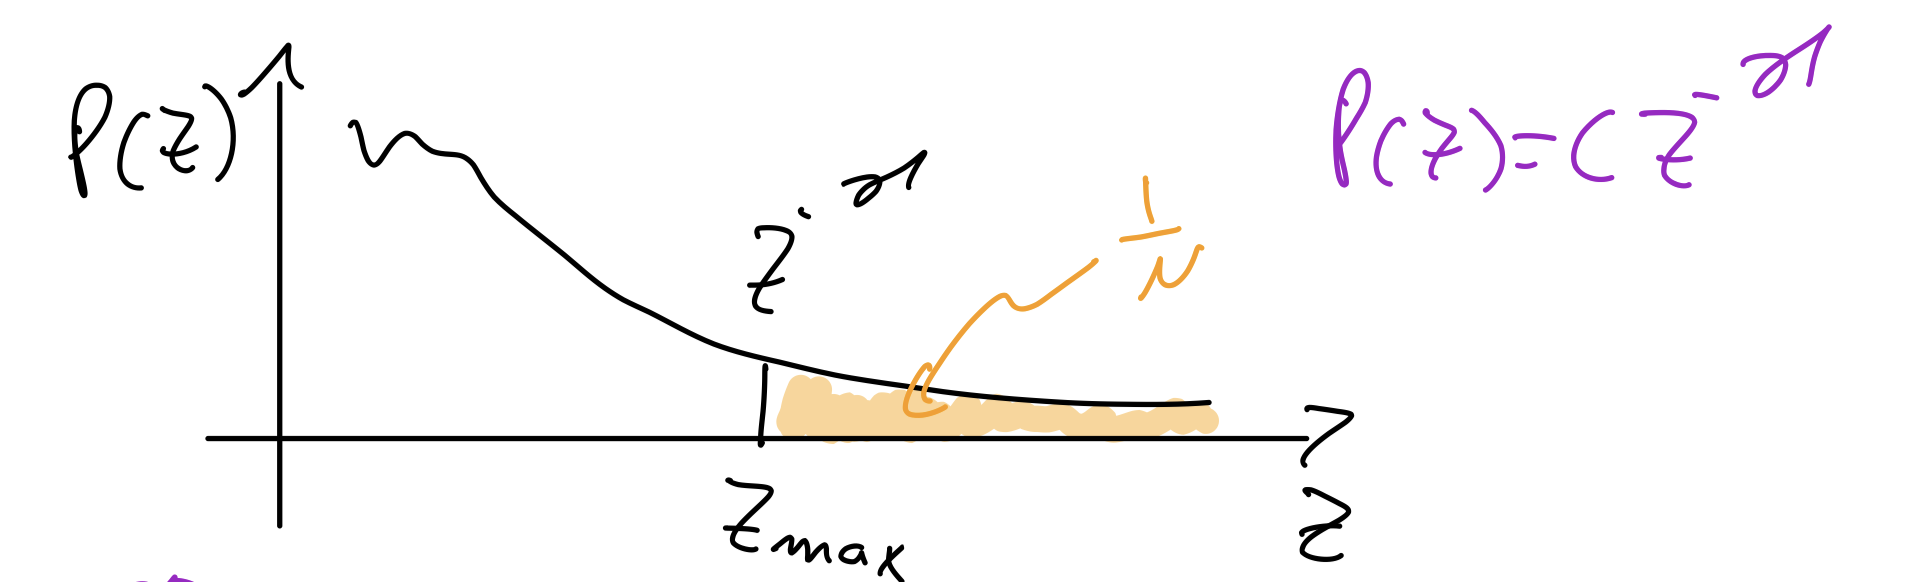
\includegraphics[scale=0.4]{Scale-free-tail}
\end{center}

\begin{proposition_exam}{Area greater than $Z_{max}$}{}In a network of N nodes, the probability to observe a node whose degree exceeds $Z_{max}$ is 
$$
\sum_{Z_{max}}^{\infty}P(Z) \approx \frac{1}{N}.
$$
\end{proposition_exam}

We can now derive a relationship for the degree of the largest node and the number of nodes N.

\begin{theorem_exam}{Largest degree in a finite network}{}In a finite network of size N, the largest degree $Z_{max}$ as a function of the network's size is given by 
$$
Z_{max} = \bigg(\frac{\gamma - 1}{C} \bigg)^{\frac{1}{1 - \gamma}}N^{\frac{1}{\gamma - 1}}.
$$
\end{theorem_exam}

\begin{proof}
First, recall the distribution for a scale-free network is $P(Z) = CZ^{-\gamma}$. Then, also note that we can use the approximation 
$$
\sum_{Z_{max}}^{\infty}P(Z) \approx \int_{Z_{max}}^{\infty}P(Z)dz = \frac{C\cdot Z^{-\gamma + 1}}{1 - \gamma}\bigg|_{Z_{max}}^{\infty} = \frac{C \cdot Z_{max}^{1 - \gamma}}{\gamma - 1}
$$
Then, we can use the previous result for the tail greater than $Z_{max}$ to get 
$$
\frac{C \cdot Z_{max}^{1 - \gamma}}{\gamma - 1} = \frac{1}{N}
$$
We can therefore solve for $Z_{max}$ as a function of N to get the desired result.
\end{proof}

Using this, we can compute the moments of a finite sized scale-free network.
\begin{proposition_exam}{Moments of a finite scale-free network}{}Fix a scale-free network of size N. Then, the first and second moment of the network is given by 
$$
\langle Z \rangle = \frac{C}{2 - \gamma}\bigg(Z_{max}^{2 - \gamma} - 1 \bigg)
$$
$$
\langle Z^2 \rangle = \frac{C}{3 - \gamma}\bigg(Z_{max}^{3 - \gamma} - 1 \bigg)
$$
\end{proposition_exam}

\begin{proof} For the first moment, we have that 
$$
\langle Z \rangle = \sum_{z=1}^{\infty}z \cdot P(Z = z) \approx \sum_{z=1}^{\infty}z \cdot P(Z = z) \approx \int_{1}^{\infty} c\cdot z^{-\gamma + 1}dz = \frac{C}{2 - \gamma}\bigg(Z_{max}^{2 - \gamma} - 1 \bigg)
$$
Then, for the second moment
$$
\langle Z^2 \rangle \approx \int_{1}^{\infty}z^2 C \cdot z^{-\gamma}dz = \frac{C}{3 - \gamma}\bigg(Z_{max}^{3 - \gamma} - 1 \bigg)
$$
\end{proof}

\begin{remark} Note that both moments $\langle Z \rangle$ and $\langle Z^2 \rangle$ depend on $Z_{max},$ which itself is a function of the number of nodes N. Therefore, the first two moments are also functions of N.
\end{remark}

We can now express the fluctuation of the degree distribution of the scale-free network.

\begin{definition_exam}{Variation of the degree distribution of scale-free network}{}
We have the coefficient of variation for the degree distribution of a scale-free network as
$$
\frac{\langle Z^2 \rangle}{\langle Z \rangle} = \frac{2 - \gamma}{3 - \gamma}\bigg(\frac{Z_{max}^{3 - \gamma} - 1}{Z_{max}^{2 - \gamma} - 1} \bigg).
$$
\end{definition_exam}

Now, we look at the effect of what happens when we remove the hub of the network. Hub removal changes the network in 2 ways 
\begin{enumerate}
\item It changes the maximum degree of the network $Z_{max} \rightarrow \tilde{Z}_{max}$ where $\tilde{Z}_{max} \leq Z_{max}$ as all nodes with degree larger than or equal to $\tilde{Z}_{max}$ has been removed. 
\item The degree distribution of the network changes from $P(Z) \rightarrow P(\tilde{Z})$ as nodes connected to the removed hubs will lose links, altering the degrees of the remaining nodes.
\end{enumerate}


\begin{definition_exam}{Fraction of hubs deleted}{} We let q be the fraction of nodes deleted from the network in descending order of degree size. That is, we say that q is the fraction of hubs deleted from the network.
\end{definition_exam}
\begin{remark} Note that we are not deleting arbitrary nodes, but the biggest nodes first!
\end{remark}

First of all, we are interested in figuring out an expression for the degree of the new hub $\tilde{Z}_{max}$ after we the fraction q of hubs.


\begin{proposition_exam}{Degree of new largest hub}{} Let q be the fraction of hubs deleted. Then, the degree of the new biggest hub as a function of q is given by
$$
\tilde{Z}_{max} = \bigg(\frac{\gamma - 1}{C} \bigg)^{\frac{1}{1 - \gamma}}q^{\frac{1}{\gamma - 1}}
$$
where q is the number of links deleted.
\end{proposition_exam}
\begin{proof} First, the number of nodes removed is given by 
$$
q \cdot N
$$
where again recall that q deletes the biggest nodes first. Therefore, this in fact deletes all the hubs between the new maximum degree $\tilde{Z}_{max}$ and the old maximum degree $Z_{max}$
$$
q \cdot N = N \sum_{\tilde{Z}_{max}}^{Z_{max}}P(Z = z) \approx N \sum_{\tilde{Z}_{max}}^{\infty}(P(Z = z) - \frac{1}{N})
$$
where the last equality uses the fact that the tail of the scale-free network between $Z_{max}$ and $\infty$ is given by $\frac{1}{N}$. Then, assuming we deleted more than one node $q >> \frac{1}{N}$, we can neglect the $\frac{1}{N}$ term and therefore 
$$
\sum_{\tilde{Z}_{max}}^{\infty}P(Z = z) \approx \int_{Z_{max}}^{\infty} C \cdot z^{-\gamma}dz = \frac{C \cdot \tilde{Z}_{max}^{1 - \gamma}}{\gamma - 1}
$$
Now, equating this result to $q \cdot N,$ we have that 
$$
q \cdot N = \frac{C \cdot \tilde{Z}_{max}^{1 - \gamma}}{\gamma - 1}
$$
We can therefore solve for $\tilde{Z}_{max}$ as a function of q.
\end{proof}

\begin{remark} We now have the maximum degree of the network after removing a fraction q of the largest hubs.
\end{remark}

We now want to compute the degree distribution of the network as it changes from $P(Z) \rightarrow P(\tilde{Z})$. However, we currently have q in terms of the number of hubs (nodes) deleted but we are interested in the fraction of links deleted as hubs are deleted. We therefore need to find a way to map these expressions to each other.

\begin{proposition_exam}{Number of links deleted by removing hubs}{}
If we remove a fraction of hubs of the network, denoted by q, we remove a fraction of the links $\utilde{q}$ given by
$$
\tilde{q} = \bigg(\frac{\gamma - 1}{C}\bigg)^{\frac{2 - \gamma}{1 - \gamma}}q^{\frac{2 - \gamma}{1- \gamma}}
$$
\end{proposition_exam}

\begin{proof} We make a big assumption that links are considered to be a random deletion of links as the network is random. Now, recall our previous formula for the \textbf{number of nodes deleted} as we delete a fraction of hubs q 
$$
q \cdot N = N \sum_{\tilde{Z}_{max}}^{Z_{max}}P(Z = z)
$$
We need to map this to see the fraction of links removed $\utilde{q}$ as we remove the fraction of hubs q. Therefore, the number of links deleted associated to the hubs removed as 
$$
\utilde{q} = \frac{N \sum_{\tilde{Z}_{max}}^{Z_{max}} z \cdot P(Z = z)}{N \langle Z \rangle} \approx \frac{1}{\langle Z \rangle} \int_{Z_{max}}^{\infty} z P(z)dz
$$
where we used the same approximation when computing the degree of the new largest hub. Recall that we computed the first moment of a finite scale-free network to be 
$$
\langle Z \rangle = \frac{C}{2 - \gamma}\bigg(Z_{max}^{2 - \gamma} - 1 \bigg)
$$
Therefore, after some algebra, we get that 
$$
\frac{1}{\langle Z \rangle} \int_{Z_{max}}^{\infty} z P(z)dz \approx \frac{\tilde{Z}_{max}^{2 - \gamma}}{1 - \tilde{Z}_{max}^{2 - \gamma}}
$$
Now, note that for $\gamma > 2$, we have that $Z_{Max} >> 1$ and therefore, we have the approximation
$$
\frac{\tilde{Z}_{max}^{2 - \gamma}}{1 - \tilde{Z}_{max}^{2 - \gamma}} \approx \tilde{Z}_{max}^{2 - \gamma}
$$
Now, note that we have an expression for the degree of the new largest hub as 
$$
\tilde{Z}_{max} = \bigg(\frac{\gamma - 1}{C} \bigg)^{\frac{1}{1 - \gamma}}q^{\frac{1}{\gamma - 1}}
$$
Applying this result, we have that 
$$
\tilde{q} \approx \tilde{Z}_{max}^{2 - \gamma} = \bigg(\frac{\gamma - 1}{C}\bigg)^{\frac{2 - \gamma}{1 - \gamma}}q^{\frac{2 - \gamma}{1- \gamma}}
$$
\end{proof}

\begin{remark} This gives us the important expression that if we remove a fraction of the hubs q, we remove a fraction $\tilde{q}$ of the links.
\end{remark}

We can now collect all the pieces we have computed in order to compute what is the critical threshold for an attack on the scale-free network.
\begin{proposition_exam}{Critical threshold for hub-removal on scale-free network}{} The critical threshold for hub-removal on a scale-free network is given by 
$$
\tilde{q}_c = 1 - \frac{1}{\frac{\langle \tilde{Z}^2 \rangle}{\langle \tilde{Z} \rangle} - 1}
$$
Importantly, the critical threshold depends on the scaling parameter of the scale-free network $\gamma.$
\end{proposition_exam}

\begin{corollary}(The critical threshold and scaling parameter are inversely related). As the scale-free network has fatter tails i.e. $\gamma \rightarrow 4,$ we have that the critical threshold drops $\tilde{q}_c \downarrow 0.$
\end{corollary}

\begin{proof} Currently, we only have the fraction of hubs deleted q. To compute the critical threshold, we require the fraction of links deleted $\tilde{q}$ as a function of q
$$
\tilde{q} = \bigg(\frac{\gamma - 1}{C}\bigg)^{\frac{2 - \gamma}{1 - \gamma}}q^{\frac{2 - \gamma}{1- \gamma}}
$$
We require the degree of the new largest hub $\tilde{Z}_{max}$ after deleting hubs
$$
\tilde{Z}_{max} = \bigg(\frac{\gamma - 1}{C} \bigg)^{\frac{1}{1 - \gamma}}q^{\frac{1}{\gamma - 1}}
$$
Finally, we require the relationship between the degree fluctuation of the distribution as a function of largest hub $Z_{max}$
$$
\frac{\langle Z^2 \rangle}{\langle Z \rangle} = \frac{2 - \gamma}{3 - \gamma}\bigg(\frac{Z_{max}^{3 - \gamma} - 1}{Z_{max}^{2 - \gamma} - 1} \bigg).
$$
From these 3 expressions, we can see that the critical threshold $q_c$ depends on the scaling parameter $\gamma.$
\end{proof}

\begin{center}
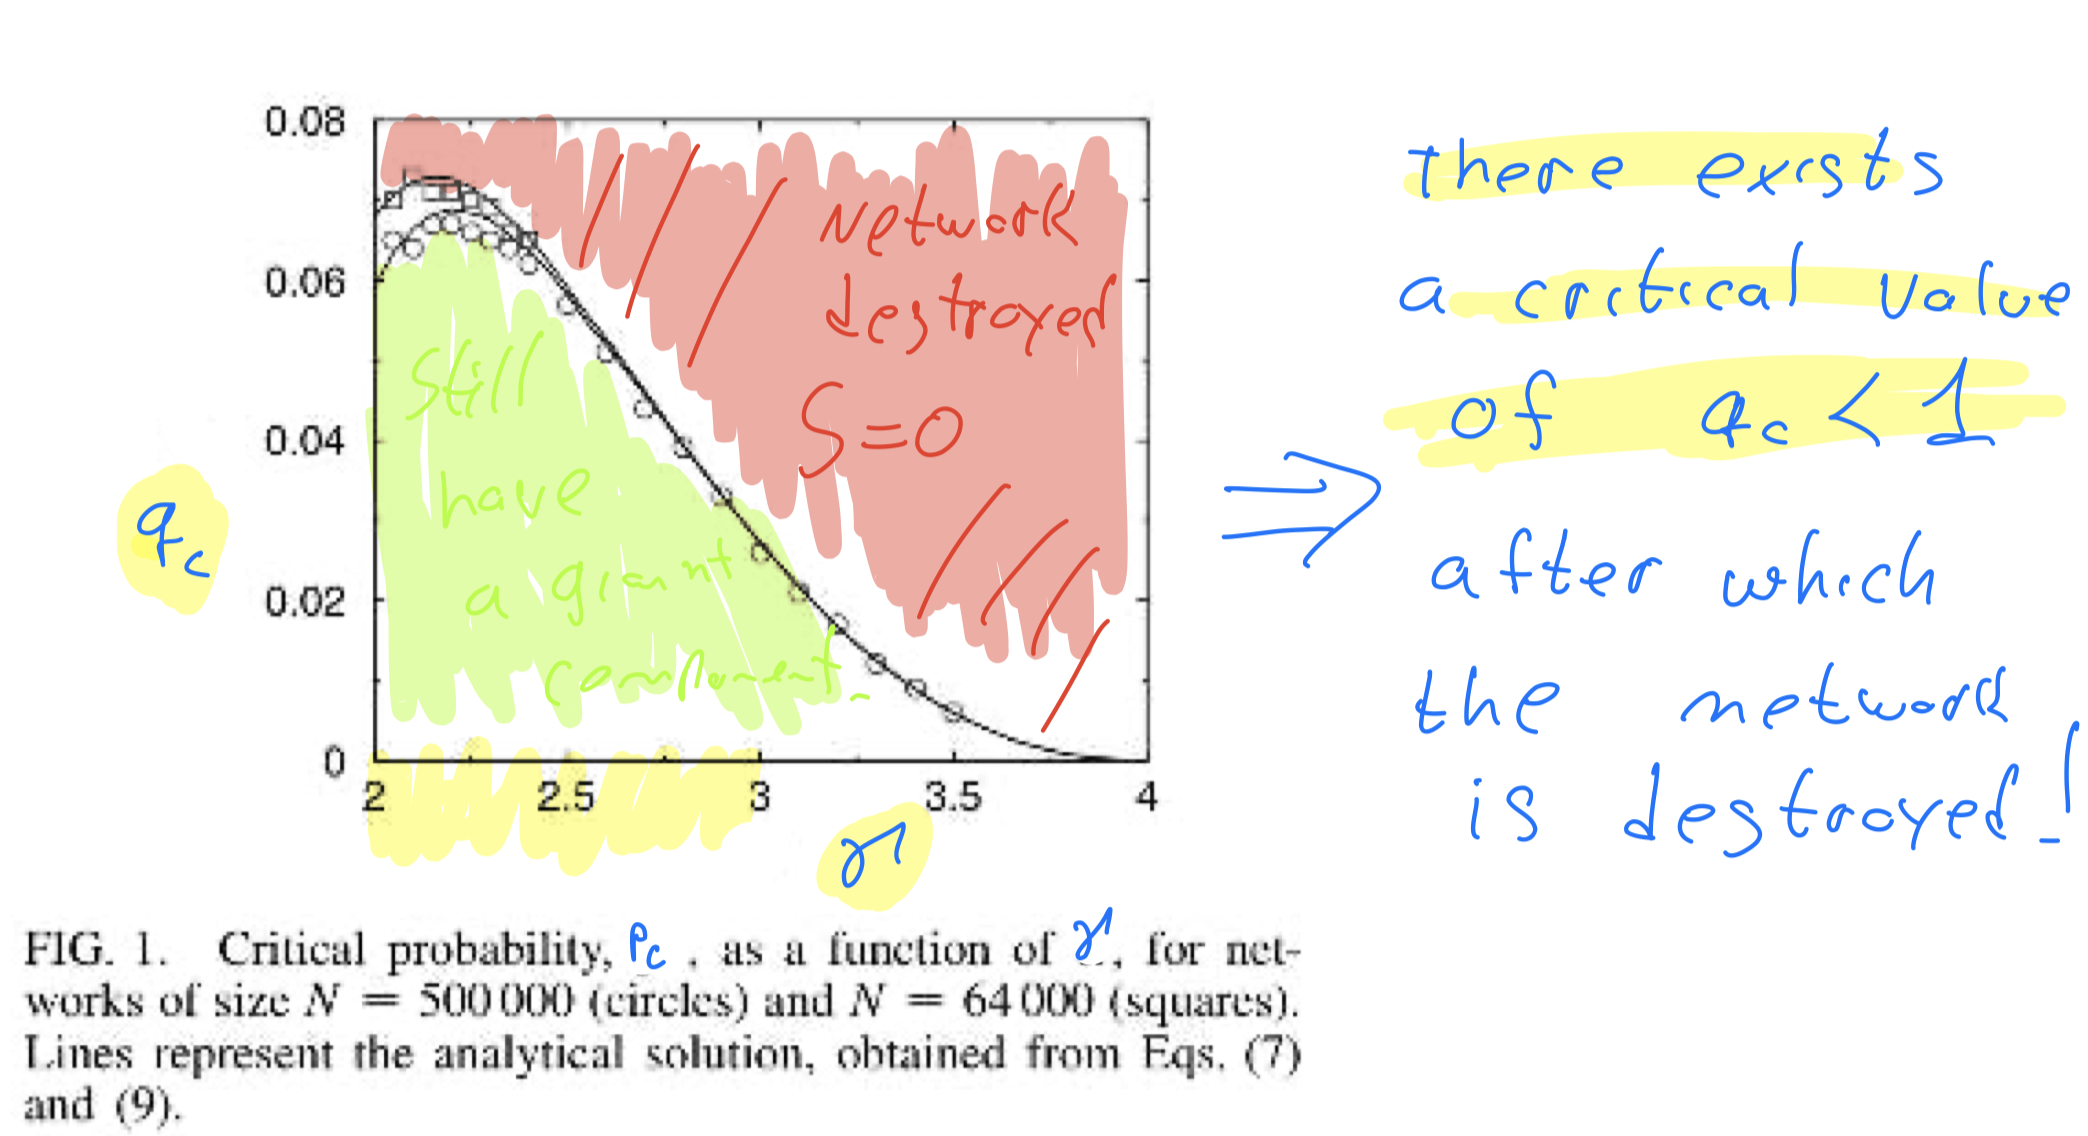
\includegraphics[scale=0.4]{Scale-free-hub-removal}
\end{center}

Therefore, we can see that the fatter the tails of the scale-free network, the lower the critical threshold to disconnect the network. This matches our intuition as if we increase the scaling parameter $\gamma \uparrow 4,$ this creates fatter tails and larger hubs, which means a targetted attack at removing these larger hubs will damage the network more.

To conclude we note that 
\begin{enumerate}
\item Scale-free networks are robust against random failures $q_c \rightarrow 1$. This is due to the fact of the heterogeneous degree distribution. Low degree nodes are far more frequent compared to high degree nodes and hence nodes that will be selected to fail are more likely to be a low degree node.
\item Scale-free networks are vulnerable to targetted attacks by removing hubs $q_c << 1.$ This occurs due to the fact that the hubs plays a large role in the network topology of keeping the network connected.
\end{enumerate}

\begin{center}
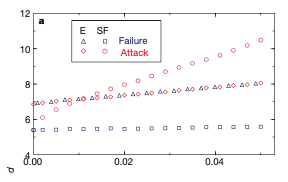
\includegraphics[scale=0.6]{Attack}
\end{center}


\lecture{13}{Threshold Models}
\section{Network Dynamics}
\section{Network Dynamics}
\subsection{Threshold Models}

We are now interested in looking at dynamics \textbf{on} networks. In particular, we now have each node i having a state $\phi_i(t)$ which evolves over time t and whose state values depends on its neighbours states $\phi_j(t).$

We are interested in seeing how do small pertubations propagate through the network and how does the network connectivity affect this. Some notable example of cascades include the adoption of new innovations, blackouts in electricity.

We first describe the binary threshold model.
\begin{definition}(Binary State Model). For each node i in our network, we define the state of node i as 
$$
\phi_i = 
\begin{cases}
1 \\
0
\end{cases}
$$
for each node $i \in \{1,2,...,N\}$.
\end{definition}

\begin{remark}We can interpret a node in state 1 as being infected and 0 as being not infected.
\end{remark}

We now describe the process at which nodes will change states as a function of their neighbours' state.

\begin{definition_exam}{Threshold Model}{}Fix a network of size N where each node has state $\phi_i(t)$ where $t \in \mathbb{N}$ is discrete time. Then the state of node i at the next point in time $t + 1$ is given by 
$$
\phi_i(t + 1) = 
\begin{cases}
1 \quad \psi_i > q_i\\
0 \quad \psi_i \leq q_i
\end{cases}
$$
where $q_i$ is the threshold level for each node i and $\psi_i = \frac{1}{Z_i}\sum_{j = 1}^{N}A_{ij}\phi_j$ is the fraction of neighbours of node i who has state $\phi_j = 1$.
\end{definition_exam}

\begin{remark}We can interpret this model as that a node becomes infected if the fraction of its neighbours that are infected is greater than its threshold value.
\end{remark}

We can assume that $q_i$ is sample from a distribution with density function $f(q)$, where this is the density of the distribution of threshold values for our network. This allows for different nodes to have different threshold values.

\begin{remark}The threshold $q_i$ for node i is fixed for all time $t \in \mathbb{N}$.
\end{remark}

We now specify a simple threshold model where the threshold value is the same for all nodes in the network.
\begin{definition_exam}{Simple Threshold Distribution}{}The simplest distribution for a threshold distribution is the indicator threshold distribution where 
$$
f(q) = \delta (q' - q)
$$
where $\delta$ is the indicator function. That is, every threshold $q_i$ in the network will have a threshold of $q^{'}$.
\end{definition_exam}

In a dynamical system, we require an initial condition. We therefore set the initial condition to be 
$$
\phi_i = 0
$$
for almost all nodes i. That is, most nodes are not infected initially.

We now define a quantity of interest when measuring our cascade.
\begin{definition_exam}{Cascade Size}{}Fix a network of size N. Let $\phi_i$ be the state of node i. Then, we define the \textbf{cascade size} $\mathcal{M}(t)$ of the network at time t as 
$$
\mathcal{M}(t) = \sum_{i=1}^{N}\phi_i(t).
$$
\end{definition_exam}

One question of interest for us is what is what is the cascade size $\mathcal{M}$ as $t \rightarrow \infty.$ What is the thermodynamic limit?

We propose that there are 2 cases that could happen to the cascade size in the limit.

\begin{proposition_exam}{Global Cascade Scenarios}{}Let $\mathcal{M}$ be the cascade size of the network of size N as $t \rightarrow \infty.$ Then, define the fraction $\frac{\mathcal{M}}{N}$ which is the fraction of nodes in state 1. We have two cases that could happen in the limit of a sparse network.
\begin{enumerate}
\item $\frac{\mathcal{M}}{N} \rightarrow 0$ as $N \rightarrow \infty$. That is, there is no global cascade (no epidemic).
\item $\frac{\mathcal{M}}{N} \rightarrow \mu > 0$ as $N \rightarrow \infty$. That is, there is a global cascade (epidemic).
\end{enumerate}
\end{proposition_exam}

\begin{remark}
In the case where $\frac{\mathcal{M}}{N} \rightarrow \mu > 0$ as $N \rightarrow \infty$, this can be interpreted as the number of nodes in state 1 grows linearly with N.
\end{remark}

We now take what we have seen and relate it to percolation theory. We shall restrict our analysis to what we call vulnerable nodes.

\begin{definition_exam}{Vulnerable Nodes}{}A node i is vulnerable if $q_i < \frac{1}{Z_i}$ where $Z_i$ is the number of neighbours of node i and $q_i$ is the threshold of node i.
\end{definition_exam}

\begin{example}We give an example of a vulnerable node. Fix a node j in the network and suppose it has degree $Z_j = 4.$ Then, we have that $1/4 = 0.25.$ Now, we sample a threshold $q_j$ from the distribution with density $f(q).$ If $q_j < 0.25,$ then, if a single neighbour of node j gets infected, then $\psi_j > q_j$ and therefore node j will become infected. That is, a node is vulnerable if one infected neighbour is sufficient to infect the node.
\end{example}

\begin{corollary}Hubs are not vulnerable as $\frac{1}{Z_i}$ will be extremely small and hence will require a small threshold value $q_i$ to be less than this.
\end{corollary}
\begin{remark}We require that infected nodes are in the same connected component in order for epidemics to spread.
\end{remark}

We can now state a result relating percolation theory to global cascades.

The general idea is that if we want a global cascade to occur, there needs to be a giant connected component comprising of vulnerable nodes in the network and this will lead to infected nodes to infect its neighbours. This is known as percolation.

\begin{theorem_exam}{Sufficient condition for global cascades}{}If \textbf{vulernable nodes} percolate in the network, then a global cascade has a positive probability of happening.
\end{theorem_exam}

We now want to compute an analytic solution to when will there be a giant component of vulnerable nodes.

\begin{definition_exam}{Probability that a node is vulnerable}{} Fix a node i. The probability that a node of degree $Z_i$ is vulnerable is 
$$
\rho_Z = F(q < \frac{1}{Z})
$$
where F is the Cumulative Distribution Function of $f(q).$
\end{definition_exam}

\begin{proposition}(Number of vulnerable nodes). The fraction of nodes with degree z that are vulnerable in the network is given by 
$$
\rho_z \cdot P(z)
$$
where $P(z)$ is the degree distribution of nodes in the network and $\rho_z$ is the probability that a node of degree $z$ is vulnerable.
\end{proposition}


Now, recall that in percolation theory, the Molloy-Reed criterion states that in order for our network to have a large giant connected component, most nodes that belong to it must be connected to 2 other nodes. Therefore, we can come up with a similar criterion for a global cascade.

\begin{proposition_exam}{Molloy-Reed Criterion for global cascade}{}Let our network only contain \textbf{vulnerable nodes}. Then, there will be a giant component of vulnerable nodes and hence a global cascade if 
$$
\frac{\langle Z^2 \rangle_{vulnerable}}{\langle Z \rangle_{vulnerable}} = \frac{\sum_{z=1}^{\infty}z^2 \cdot \rho_z \cdot P(Z = z)}{\sum_{z=1}^{\infty}z \cdot \rho_z \cdot P(Z = z)} \geq 2
$$
where $\langle Z \rangle_{vulnerable}$ is the first moment of the degree of vulnerable nodes.
\end{proposition_exam}
\begin{remark}
Hence, we require each vulnerable node to be connected to at least 2 more vulnerable nodes in order for a giant single connected component of vulnerable nodes to emerge.
\end{remark}

Running empirical results, we can observe that there exists a transition point $q^*$ where a global cascade occurs.

\begin{proposition_exam}{Percolation threshold}{}When we vary the threshold value q from $0 \rightarrow 1$, we find that there is a sharp transition point $q=q^*$ where a global cascade stops.
\end{proposition_exam}
\begin{remark} Note that a cascade stops as we \textbf{increase} the threshold q, as it is harder for a node to become infected as its threshold goes up.
\end{remark}


\lecture{14}{Epidemic Spreading}
\section{Network Dynamics}
\subsection{Hypotheses under SIR Model}
There are two fundamental hypotheses underlying the epidemic models.

\begin{definition_exam}{Compartmentalization}{}An individual can be classed in one of three states 
\begin{enumerate}
\item Susceptible (S): Healthy individuals who have not yet contacted the disease;
\item Infectious (I): Contagious individuals who have contacted the disease and hence can infect other;
\item Recovered (R): Individuals who have been infected before and have recovered from the disease.
\end{enumerate}
\end{definition_exam}

Individuals can move between these states. We can specify parameters $\mu$ for the recovery rate and $\lambda$ for the infection rate.

\begin{definition_exam}{Homogenous Mixing}{}Each individual has the same chance of coming into contact with an infected individual. 
\end{definition_exam}

With homogenous mixing, we do not need to know the precise contact network on which the disease spreads. Hence, anyone can infect anyone else. 

We define two forms of dynamics.

\begin{enumerate}
\item We can infect at a rate $\lambda$ from state $(S) \rightarrow (I)$
\item We can recover at a rate $\mu$ from state $(I) \rightarrow (R).$
\end{enumerate}

\begin{definition_exam}{Fraction of states}{} We define the set of measures of interest in our SIR model

$$
\begin{cases}
s = \frac{\text{\# of nodes in state }\phi = S}{N}\\\\
\rho = \frac{\text{\# of nodes in state }\phi = I}{N}\\\\
r = \frac{\text{\# of nodes in state }\phi = R}{N}\\\\
\end{cases}
$$
\end{definition_exam}

This approach differes to agent based models where we have discrete space and time. In our set up, we have discrete space but continuous time.

\subsection{SIR Models}
We can now define our epidemic spreading models based on the 3 states. We can define a set of differential equations to model how the dynamics of our model plays out.
\begin{definition_exam}{SIR Model}{}Let $\overline{Z}$ be the number of contacts per unit of time. Let $\lambda$ be the rate of infection. Let $\mu$ be the rate of recovery. Then, under the hypotheses of compartmentalization and homogenous mixing, we have the set of differential equations
$$
\begin{cases}
\frac{ds}{dt} = -\lambda \overline{Z}s(t)\rho(t)\\\\
\frac{d\rho}{dt} = +\lambda \overline{Z}s(t)\rho(t) - \mu \rho(t)\\\\
\frac{dr}{dt} = +\mu\rho(t)
\end{cases}
$$
where $s(t) + \rho(t) + \mu(t) = 1$ for all $t \in \mathbb{T}.$ The initial conditions for this set of 3 non-linear ODEs are 
$$
\begin{cases}
s(t = 0) = S_0 \approx 1\\
\rho(t = 0) = 1 - S_0 \approx 0\\
r(t = 0) = 0.
\end{cases}
$$
\end{definition_exam}

\begin{remark}Here, the rate of infection $\lambda$ and rate of recovery $\mu$ are control parameters for our model.
\end{remark}

This is a well-defined mathematical problem whereby we can expect that eventually all nodes in our network will reach the recovered state as long as the rate of infection and rate of recovery is not zero.

We are interested in the limit of the SIR model.
\begin{center}
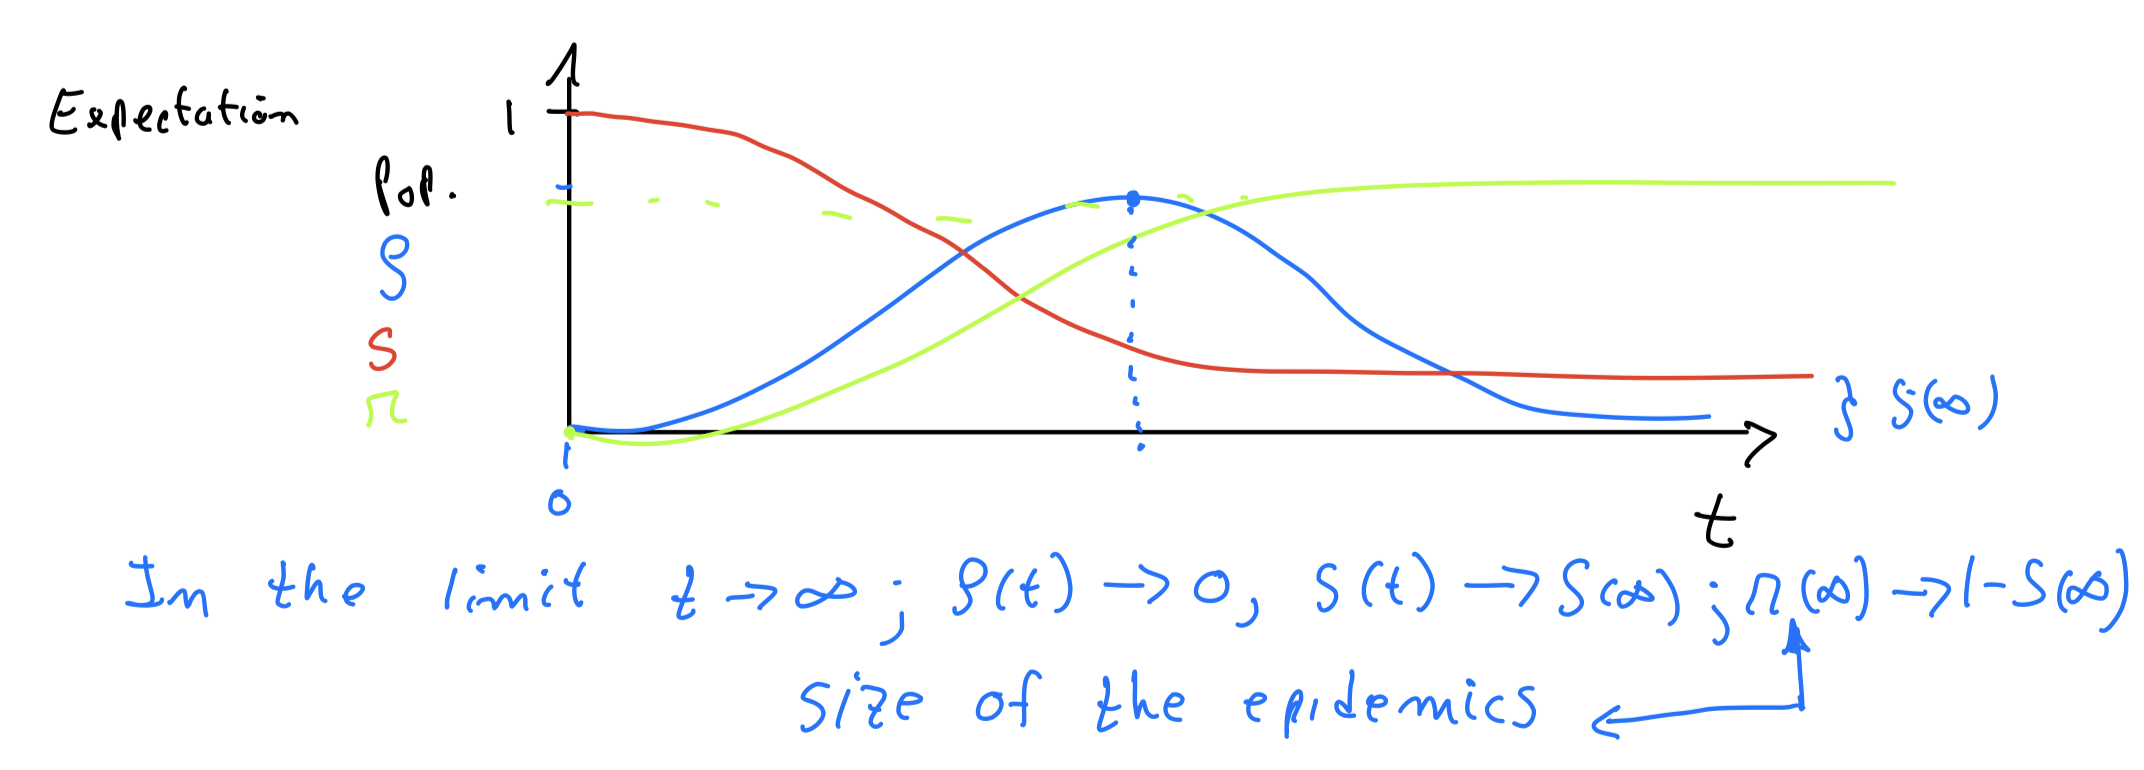
\includegraphics[scale=0.4]{SIR-Limit}
\end{center}

\begin{proposition_exam}{Limiting behaviour of SIR Model}{}Let s be fraction of susceptible, $\rho$ be the fraction of infected people, and r as the fraction of recovered people. In the limit as $t \rightarrow \infty$
$$
\begin{cases}
\rho(t) \rightarrow 0 \\\\
s(t) \rightarrow s(\infty) = e^{-\frac{\lambda}{\mu}\overline{Z}r(\infty)}\\\\
r(\infty) \rightarrow 1 - s(\infty) = 1 - e^{-\frac{\lambda}{\mu}\overline{Z}r(\infty)}
\end{cases}
$$
\end{proposition_exam}

\begin{proof} We want to remove the time component in our analysis. In particular, we want to analyse the limiting behaviour of the susceptible and recovered fraction of the population. First, we derive the limiting behaviour of the fraction of susceptible people
$$
\frac{ds}{dt}\frac{dt}{dr} = \frac{ds}{dr} = \frac{-\lambda \overline{Z}}{\mu}s
$$
which is a seperable equation to solve. We can therefore derive that 
$$
s(r) = s(0)e^{-\frac{\lambda \overline{Z}}{\mu}r}
$$
where $s(0) = 1.$ Then, we can take limits as $r \rightarrow \infty$
$$
\lim_{r \rightarrow \infty}s(r) = s(\infty) = e^{-\frac{\lambda \overline{Z}}{\mu}r(\infty)}.
$$
Now, we analyse the limiting behaviour of the fraction of recovered people 
$$
r(\infty) = 1 - s(\infty) - \rho(\infty) = 1 - s(\infty) = 1 - e^{-\frac{\lambda \overline{Z}}{\mu}r(\infty)}.
$$
\end{proof}

We are now interested in the epidemic threshold. In fact, we can describe that there is a bifurication at the point $\frac{\lambda}{\mu} = \frac{1}{\overline{Z}}$ which is the epidemic threshold.
\begin{proposition_exam}{Transition phase into epidemic regime}{}To switch into a epidemic regime, we require that 
$$
\sigma_c = \frac{1}{\overline{Z}} > \frac{\lambda}{\mu}
$$
where $\lambda$ is the rate of infection, $\mu$ is the rate of recovery, and $\overline{Z}$ is the number of contacts per unit time. We define $\sigma_c$ as the epidemic threshold.
\end{proposition_exam}

\begin{proof} Recall that in the limit, we had that 
$$
r(\infty) = 1 - e^{-\frac{\lambda}{\mu}\overline{Z}r(\infty)}
$$
We now solve this self-consistent equation by differentiating it and evaluating it at $r(\infty) = 0$ and checking whether is the gradient greater than 1. This is so that we have a non-trivial solution to the equation 
$$
\frac{d}{dr(\infty)} \bigg( 1 - e^{-\frac{\lambda}{\mu}\overline{Z}r(\infty)}\bigg)\bigg|_{r(\infty) = 0} > 1
$$
$$
= \frac{\lambda \overline{Z}}{\mu}e^{-\frac{\lambda}{\mu}\overline{Z} \cdot 0} > 1
$$
which gives us 
$$
\frac{\lambda \overline{Z}}{\mu} > 1
$$
and therefore, we get the desired result that 
$$
\sigma = \frac{\lambda}{\mu} > \frac{1}{\overline{Z}}
$$
\end{proof}

\begin{center}
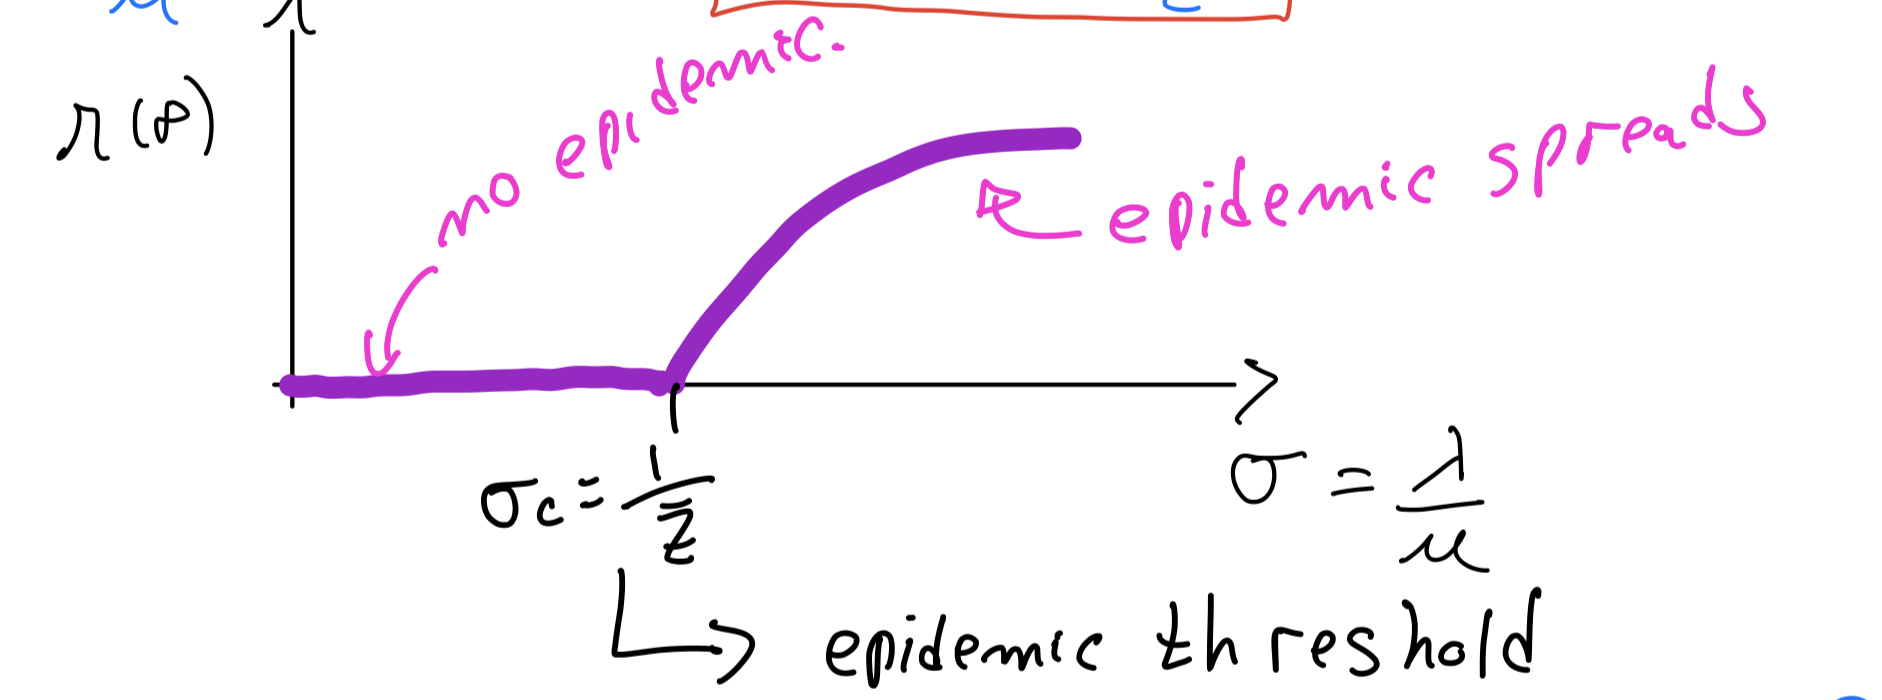
\includegraphics[scale=0.4]{epidemic-threshold}
\end{center}

\begin{remark}Keeping our contacts by social distancing low $\overline{Z}$ will stop us from entering the epidemic regime.
\end{remark}

\subsection{SIR Models with Networks}

We now want to relax the homogenous mixing assumption and introduce a random graph with a fixed degree distribution P(Z). 

\textbf{We will now treat each degree class Z separately.}

\begin{definition_exam}{Degree class of states}{} Let P(Z) be the degree distribution of the random graph. We define the SIR states as 
$$
\{s(t), \rho(t), r(t)\} = \sum_{z=1}^{\infty}P(z)\{s_z(t), \rho_Z(t), r_z(t) \}
$$
where $s_z(t) + \rho_z(t) + r_z(t)$ for each degree z and t.
\end{definition_exam}

We also generalise the number of contact per unit time $\overline{Z}.$

\begin{definition}(Number of contact per unit time). We generalise the number of contact per unit time as 
$$
\theta(t) = \sum_{z=1}^{\infty}\frac{zP(Z=z)\rho_z(t)}{\langle Z \rangle}
$$
is the probability to be linked to an infected node.
\end{definition}

\begin{remark} Note that the probability to be infected depends on the degree class.
\end{remark}

We can now define a new set of differential equations for the SIR model.


\begin{definition_exam}{SIR Model with degrees}{}Let $\overline{Z}$ be the number of contacts per unit of time. Let $\lambda$ be the rate of infection. Let $\mu$ be the rate of recovery. Then, under the hypotheses of compartmentalization and homogenous mixing, we have 
$$
\begin{cases}
\frac{ds_{z}}{dt} = -\lambda \overline{Z}s \theta(t)\\\\
\frac{d\rho_{z}}{dt} = +\lambda \overline{Z}s\theta(t) - \mu \rho_z\\\\
\frac{dr_{z}}{dt} = +\mu\rho_z
\end{cases}
$$
where $s_z(t) + \rho_z(t) + r_z(t) = 1$ for all $t \in \mathbb{T}.$ The initial conditions for this set of 3 non-linear ODEs are 
$$
\begin{cases}
s_z(t = 0) = S_0 \approx 1\\
\rho_z(t = 0) = 1 - S_0 \approx 0\\
r_z(t = 0) = 0.
\end{cases}
$$
\end{definition_exam}

We can solve to find the epidemic threshold for the SIR model with degrees.
\begin{proposition_exam}{Epidemic Threshold in network SIR Model}{}
Define epidemic threshold as $\sigma_c = \frac{\langle Z \rangle}{\langle Z^2 \rangle}.$ Then, percolation occurs if 
$$
\sigma = \frac{\lambda}{\mu} > \frac{\langle Z \rangle}{\langle Z^2 \rangle} = \sigma_c.
$$
\end{proposition_exam}

\begin{proof} First, note that $\frac{dr_{z}}{dt} = +\mu\rho_z$ can be integrated on both sides to show that
\begin{equation}
\int \rho_z(t)dt = \frac{r_z}{\mu}
\tag{*}
\end{equation}
Then, we have that 
\begin{equation}
\phi(t) = \int \theta(t)dt = \frac{1}{\langle Z \rangle}\sum_{z=1}^{\infty}z \cdot P(Z = z) \int \rho_z(t)dt = \frac{1}{\langle Z \rangle}\sum_{z=1}^{\infty}z \cdot P(Z = z)\frac{r_z}{\mu}
\tag{**}
\end{equation}
where we used (*) for the last equality. We will use this expression for $\phi(t)$ later.

Now, look at the separable equation 
$$
\frac{ds_{z}}{dt} = -\lambda \overline{Z}s \theta(t)
$$
we can solve this to get 
\begin{equation}
s_z(t) = s_z(0)e^{-\lambda z \int \theta(t)dt}
\tag{***}
\end{equation}

We are now interested in the rate of probability of being linked to an infected node, so we then differentiate equation (*) with respect to t 
$$
\frac{d\phi}{dt} = \frac{1}{\langle Z \rangle}\sum_{z=1}^{\infty}z \cdot P(Z = z)\frac{d}{dt} \frac{r_z}{\mu} = \frac{1}{\langle Z \rangle}\sum_{z=1}^{\infty}z \cdot P(Z = z) \rho_z(t)
$$
where the last equation arises because $\frac{dr_{z}}{dt} = +\mu\rho_z.$ Then, using the fact that $s_z(t) + \rho_z(t) + r_z(t) = 1$, we have that 
$$
= \frac{1}{\langle Z \rangle}\sum_{z=1}^{\infty}z \cdot P(Z = z) \bigg(1 - s_z(t) - r_z(t) \bigg) =  \frac{1}{\langle Z \rangle}\sum_{z=1}^{\infty}z \cdot P(Z = z) -  \frac{1}{\langle Z \rangle}\sum_{z=1}^{\infty}z \cdot P(Z = z) \cdot s_z(t) -  \frac{1}{\langle Z \rangle}\sum_{z=1}^{\infty}z \cdot P(Z = z) \cdot r_z(t)
$$
$$
= \frac{\langle Z \rangle}{\langle Z \rangle} -  \frac{1}{\langle Z \rangle}\sum_{z=1}^{\infty}z \cdot P(Z = z) \cdot s_z(t) -  \frac{1}{\langle Z \rangle}\sum_{z=1}^{\infty}z \cdot P(Z = z) \cdot r_z(t)
$$
Now, using equation (**) and (***) we get 
$$
\frac{d\phi}{dt} = 1 - \frac{1}{\langle Z \rangle}\sum_{z=1}^{\infty}z \cdot P(Z = z) \cdot s_z(0)e^{-\lambda z \int \theta(t)dt} - \mu \cdot \phi(t)
$$
Now, we know that as $t \rightarrow \infty,$ the number of infected falls to zero $\rho_z(\infty) = 0$ and this also implies that $\lim_{t \rightarrow \infty}\frac{d\phi}{dt} = 0.$ Furthermore, by assumption, $s_z(0) = 1.$ Hence, we have that 
$$
0 = 1 - \mu \cdot \phi(\infty) - \frac{1}{\langle Z \rangle}\sum_{z=1}^{\infty}zP(Z = z)e^{-\lambda z \phi(\infty)}
$$
Now, we can see that a non-trivial solution for $\phi(\infty)$ exists if 
$$
\frac{d}{d\phi(\infty)}\bigg(\frac{1}{\mu} - \phi(\infty) - \frac{1}{\langle Z \rangle \mu}\sum_{z=1}^{\infty}zP(Z = z)e^{-\lambda z \phi(\infty)} \bigg)|_{\phi(\infty) = 0} > 1
$$
$$
= \frac{d}{d\phi(\infty)} \bigg(- \frac{1}{\langle Z \rangle \mu}\sum_{z=1}^{\infty}zP(Z = z)e^{-\lambda z \phi(\infty)} \bigg)|_{\phi(\infty) = 0} > 1
$$
$$
= \frac{1}{\langle Z \rangle}\sum_{z=1}^{\infty}zP(Z = z)\frac{\lambda z}{\mu}e^{-\lambda z(0)} > 1 = \frac{\lambda}{\mu}\frac{1}{\langle Z \rangle}\sum_{z=1}^{\infty}z^2P(Z = z) > 1
$$
and therefore, we have that 
$$
\sigma = \frac{\lambda}{\mu} > \frac{\langle Z \rangle}{\langle Z^2 \rangle} = \sigma_c.
$$
\end{proof}

\begin{center}
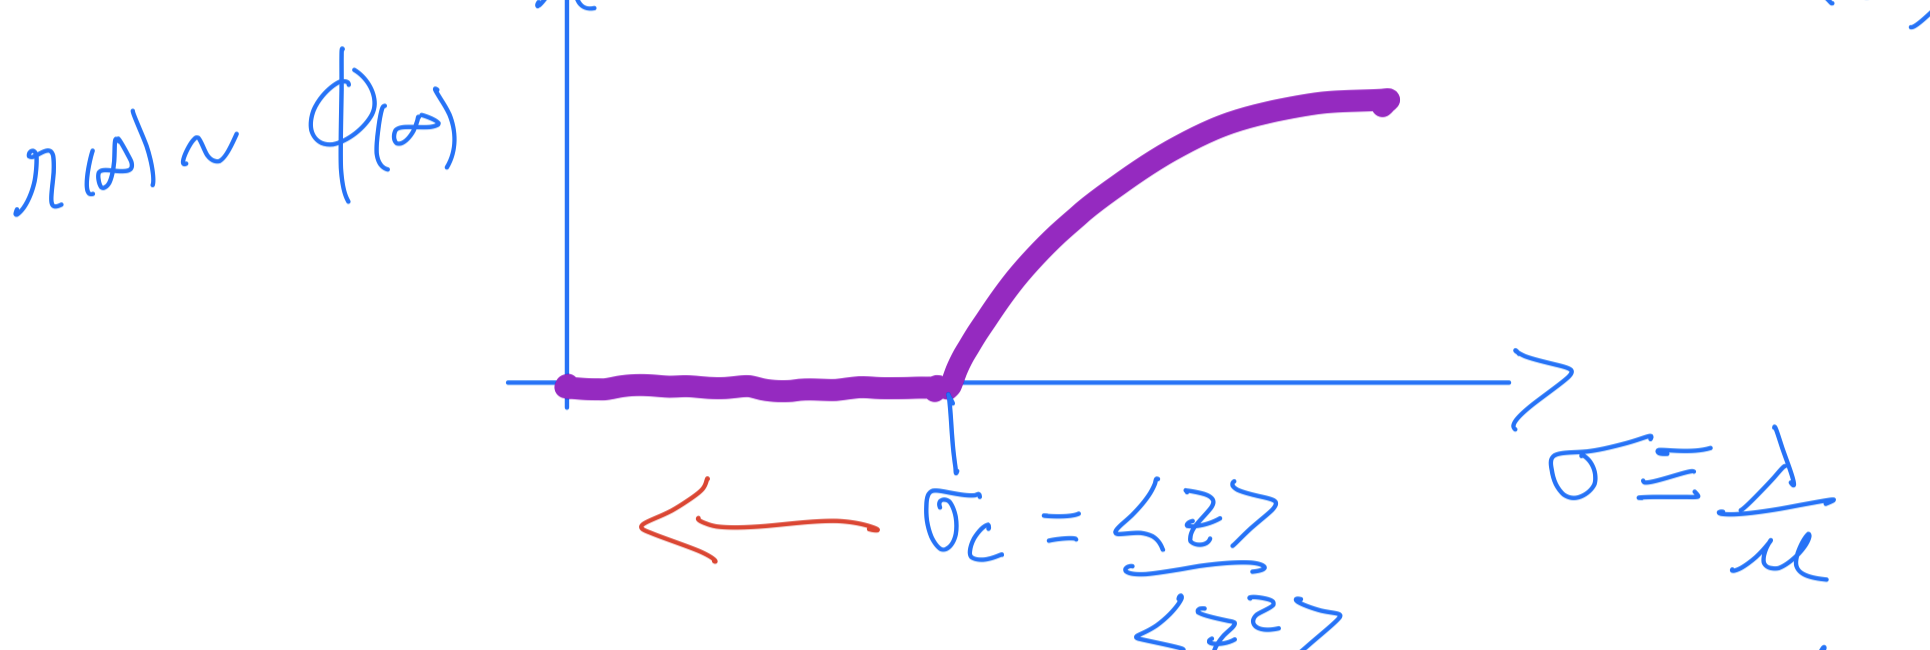
\includegraphics[scale=0.4]{epidemic-network-threshold}
\end{center}

We now come to a startling conclusion.

\begin{proposition_exam}{Global cascades occur easily in scale-free networks}{}For a scale-free network where $2 \leq \gamma \leq 3$, we have that the epidemic threshold $\sigma_c \rightarrow 0$.
\end{proposition_exam}
\begin{proof} First, recall that the epidemic threshold is 
$$
\sigma_c = \frac{\langle Z \rangle}{\langle Z^2 \rangle}
$$
Furthermore, in scale-free networks, the second moment diverges $\langle Z^2 \rangle \rightarrow \infty.$ Therefore, $\sigma_c \rightarrow 0$ as the second moment diverges.
\end{proof}

Hence, any disease leads to an epidemic! If a hub gets infected, everyone else will get infected too.

\subsection{Connections of SIR Model to percolation theory}

We connect our results to what we saw in percolation theory. We now assume that each node remains infected for a time period $T \sim \frac{1}{\mu},$ which is the inverse of the recovery rate.

\begin{proposition_exam}{Probability of disease transmission}{}The probability of a disease being transmission to neighbours is given by 
$$
p = \frac{\lambda}{\mu} > 0.
$$
\end{proposition_exam}
\begin{proof}  The probability of transmission to neighbours is the complement of the time not being infected 
$$
p = 1 - (1 - \lambda dt)^{\frac{T}{dt}} \approx 1 - e^{\lambda dt \frac{T}{dt}} \approx 1 - e^{\frac{\lambda}{\mu}} \approx \frac{\lambda}{\mu} = \sigma
$$
for $\frac{\lambda}{\mu} > 0.$
\end{proof}

We can now compute the percolation threshold where we infect a neighbour with probability p.


\begin{theorem_exam}{Critical percolation threshold}{} The critical percolation threshold is given by 
$$
P_c \approx \frac{\langle Z \rangle}{\langle Z^2 \rangle}.
$$
\end{theorem_exam}
\begin{proof} Recall that 
$$
P_c = \frac{1}{\frac{\langle Z^2 \rangle}{\langle Z \rangle} - 1} \approx \frac{\langle Z \rangle}{\langle Z^2 \rangle} = \sigma_c
$$
for $\langle Z^2 \rangle >> \langle Z \rangle,$ which holds for scale-free networks.
\end{proof}

Therefore, we can conclude that if the probability of infection 
$$
p \approx \frac{\lambda}{\mu} > p_c \approx \frac{\langle Z \rangle}{\langle Z^2 \rangle}
$$
then a global cascade occurs. This is the same result as we saw before in the percolation threshold for a Bethe lattice!

\lecture{15}{Dynamics on discrete models}
\section{Dynamics on networks}
\section{Dynamics on networks}
\subsection{Dynamics on discrete models}

We now want to generalise the threshold model from before. We describe the set up of the system.
\newline

Suppose we had i = 1,...,N nodes in a sparse network. Denote $k_i = z_i$ as the degree of node i. Denote $P(K) = P(Z)$ as the degree distribution where $K_{max} = Z_{max} << N$, that is, we are in a sparse network where not a single node is not connected to all nodes.

Denote $\phi_i \in [0,1]$ as the binary state of nodes.

For a node i, denote $m_i$ by the number of neighbours of node i in state 1 given by 
$$
m_i = \sum_{j=1}^{N}A_{ij}\phi_j
$$

In fact, we can cast this into the fraction of neighbours of node i in state 1 by dividing by the degree of node i:
$$
\frac{m_i}{k_i}
$$

\begin{definition_exam}{Transition probabilities}{} For a given node i in the network, denote $F_{k,m}$ as the transition probability from going to state 0 to state 1, which depends on the degree k and number of neighbours in state 1, denoted by m, of node i.
\newline

Denote $R_{k,m}$ as the transition probability to go from state 1 to state 0 for node i, which depends on the degree k and number of neighbours in state 1, denoted by m, of node i.
\end{definition_exam}

We now define the main observation of interest we wish to investigate.
\begin{definition_exam}{Fraction of infected nodes}{}Let $t \in \mathbb{Z}.$ Then, $\rho(t)$ is the fraction of nodes in state 1 given by 
$$
\rho(t) = \frac{1}{N}\sum_{i=1}^{n}\phi_i(t)
$$
\end{definition_exam}


\subsection{Continuous-Time Approximations}
We wish to now analyse the investigation between parameters of our models and the connection between networks and dynamics.

We can think about this as for $N \rightarrow \infty$, the step time $dt \sim \frac{1}{N} \rightarrow 0$, also known as the thermodynamic limit. Now, in each time step dt, one random node is updated and after time step t, all n nodes are updated.

However, it is difficult to algorithmically analyse this and we are required to map thse discrete states into continuous differential equations. We therefore make two key approximations in the following approximation methods we will soon see 
\begin{enumerate}
\item We have a random graph with a fixed degree distribution 
\item We have the transition probabilities $R_{k,m}$ and $F_{k,m}$ for nodes with degree k and number of activated neighbours m in a time interval dt.
\end{enumerate}



We will look into 3 approximation methods for this.
\subsubsection{Mean-Field Approximations}

First, recall the probability mass function of something we will need.
\begin{definition}(Binomial Mass Function). The binomial mass function with k trials, m successes, and probability of success being q is given by 
$$
B_{k,m}(q) = {k \choose m}q^m(1 - q)^{k - m}
$$
\end{definition}

The quantity of interest is the number of nodes infected at any given point in time. The key idea is to \textbf{sum over degree classes the number of infected nodes}.

\begin{proposition_exam}{Mean-Field Approximation}{}Construct $K = 1,2,...,K_{max}$ number of equations for each degree class of the network. Denote by $\rho_k$ the fraction of infected nodes in with degree k. Then, we have a mean-field equation for each degree class separately given by 
\begin{equation}
\frac{d}{dt}\rho_k = -\rho_k\sum_{m=0}^{K}R_{k,m}B_{k,m}(\omega) + (1 - \rho_k)\sum_{m=0}^{K}F_{k,m}B_{k,m}(\omega)
\tag{*}
\end{equation}
where $B_{k,m}(q)$ is the Binomial distribution density function and $\omega$ is the probability of a node being infected given by 
$$
\omega = \big\langle \frac{k\rho_k}{\langle k \rangle} \big\rangle
$$
\end{proposition_exam}

\begin{remark}In equation (*), nodes will become infected (recovered) proportionally depending on the number of infected (recovered) nodes in the same degree class. We assign nodes in state 1 based on the Binomial probability mass function. Furthermore, all nodes have the same probability of being infected which is given by $\omega.$
\end{remark}

A big key assumption on this model is that there is no correlation between the state of node X and the state of neighbours of node X. This does not make sense and hence we seek to relax this assumption.

\subsubsection{Pair Approximations}
We now incorporate the idea of correlation between pair of neighbours into our model. That is, we look at each pair of nodes and consider their interaction independently. This comes from an idea in Physics where in the 1D Ising model, there are regions of atoms consisting of only spin ups or spin downs.

Before, we assumed the probability of a node being infected $\omega$ was constant for all nodes. We now have the probability
\begin{proposition_exam}{Pair Approximation Equations}{}
We define the pair approximation equations as 3 sets of differential equations where now the probability of infection and recovery are also evolving over time. The pair approximation equations are given by
\begin{equation}
\begin{cases}
\frac{d}{dt}\rho_k = -\rho_k\sum_{m=0}^{K}R_{k,m}B_{k,m}(q_k) + (1 - \rho_k)\sum_{m=0}^{K}F_{k,m}B_{k,m}(p_k)\\
\frac{d}{dt}p_k = \sum_{m=0}^{K}[p_k - \frac{m}{k}][F_{k,m}B_{k,m}(p_k) - \frac{\rho_k}{1 - \rho_k} R_{k,m}B_{k,m}(q_k)] + \beta^s(1 - p_k) - \gamma^sp_k\\
\frac{d}{dt}q_k = \sum_{m=0}^{K}[q_k - \frac{m}{k}][R_{k,m}B_{k,m}(q_k) - \frac{1 - \rho_k}{\rho_k} F_{k,m}B_{k,m}(p_k)] + \beta^i(1 - q_k) - \gamma^iq_k
\end{cases}
\tag{*}
\end{equation}
\end{proposition_exam}

We now have $3.K_{max}$ equations, that is, 3 times more equations compared to the Mean-field approximation model.

\subsubsection{Approximate Master Equations}
Master equations are used to describe the time evolution of a system that can be modelled as being in a probabilistic combination of states at any given time and the switching between states is determined by a transition rate matrix.

The equations are a set of differential equations – over time – of the probabilities that the system occupies each of the different states.

Recall that $k_{max}$ is the number of degree classes for our network. Then, the number of equations in the master equations is given by $k_{max}^2 << N.$

\lecture{16}{Games on networks}
\section{Dynamics on networks}
\subsection{Games on networks}

We are interested in the intersectin of game theory and network theory.
\begin{definition_exam}{Game}{}A game between two players i and j is defined by 
\begin{enumerate}
\item A set of feasible strategies $\{e_1,e_2,...,e_Q\}$
\item A payoff matrix 
$$
M_{e_{i}e_{j}}
$$
which is of size Q by Q where Q is the total number of available strategies.
\end{enumerate}
\end{definition_exam}

We can define the standardised pay-off matrix for 2 players.
\begin{definition}(Standard pay-off matrix). Suppose we have 2 players with 2 feasible strategies. Then, the standardised payoff matrix is 
$$
M_{e_{i}, e_{j}} = 
\begin{bmatrix}
1 & 0\\
b & 0
\end{bmatrix}
$$
where b is a parameter to vary.
\end{definition}

We can think of the parameter b in the standard payoff matrix as the temptation to defect.

\begin{lemma}For all $b > 1$, the dominant strategy is to defect.
\end{lemma}

\begin{remark}The Nash equilbrium is for both players to defect, an outcome worse off from the optimal outcome for both players.
\end{remark}

We now investigate on how can we ensure co-operation. In particular, we can repeatedly play games to ensure cooperation.

We now describe the setup of repeated games in a network. For a given network of size N, initialise 50\% of nodes to have their strategy to be to cooperate whereas the remaining 50\% to choose defect for their strategy. We define the adjacency $A_{ij}$ for this network. 

\begin{definition}(Accumulated payoff). The accumulated payoff for node i in a single round of playing is given by 
$$
S_i = \sum_{j=1}^{N}A_{ij}M_{e_{i}e_{j}}.
$$
\end{definition}

\begin{remark}Note that due to the network setting, a node will always play games against the same neighbours.
\end{remark}
We now describe the strategy update regime. 

\begin{proposition}(Strategy update). For a given node i, pick a neighbour j randomly. Then, if the neighbour's payoff $p_j > p_i$ is greater than node i, the node i will adopt their neighbour j's strategy \textbf{with probability}
$$
\mathbb{P} = \frac{S_j - S_i}{S_{max}}
$$
where $S_j - S_i$ is the difference in accumulated payoff and $S_{max}$ is the total payoff that could have occured, which is given by $S_{max} = bZ_{max} = b.\max\{Z_i, Z_j\}.$
\end{proposition}

We can then play $\max\{Z_i, Z_j\}$ rounds between node i and j.

Finally, we can measure for $N \rightarrow \infty$ and $t \rightarrow \infty$, the expected number of cooperations, which is defined as the frequency of cooperations in the network.

We find the first result from games in networks.
\begin{proposition_exam}{Cooperation in scale-free networks}{}Degree heterogeneity favours cooperation in scale-free networks.
\end{proposition_exam}
\begin{proof}(Sketch). Think of a network with 2 massive hubs of a star graph set up. Suppose one hub node X has a strategy to defect and the other hub Y has a strategy to cooperate. All of X's neighbours will continuously defect against X whereas all of Y's neighbours will co-operate. Eventually, Y will have a higher pay-off compared to X and therefore hub X will adopt Y's strategy to cooperate.
\end{proof}

Through empirical results, we see that as we increase the temptation to defect, defection prevails in a regular graph. However, in a scale-free network, we see that cooperation prevails.


\lecture{17}{Continuous-time Dynamics on Networks}
\section{Dynamics on networks}
\subsection{Linear Systems Review}

\subsection{Continuous-time Dynamics on Networks}
First, recall the basic definition of a linear system.
\begin{definition_exam}{Linear System}{}Let $\utilde{x} \in \mathbb{R}^n$ be a state variable. We define a linear system to be the ordinary differential equation 
$$
\frac{d\utilde{x}}{dt} = A\utilde{x}
$$
where $A \in \mathbb{R}^{n \times n}$ is the evolution operator.
\end{definition_exam}

We now extend the set up to also include the network properties into the dynamics of the system.

\begin{definition_exam}{Dynamics on networks with coupling}{}Define a network with N nodes. We denote $x_i$ to be the state of node i. Then, the dynamics of each state $x_i$ is given by
$$
\frac{dx_i}{dt} = f_i(x_i) + \sum_{j=1}^{N}A_{ij}g_{ij}(x_i,x_j)
$$
where $f_i(x_i)$ is the internal dynamics of the node i and $\sum_{j=1}^{N}A_{ij}g_{ij}(x_i,x_j)$ models the coupling effect of all the neighbours j of node i.
\end{definition_exam}

\begin{remark}With N nodes, we have a set of N ODE equations.
\end{remark}

This setup differs to the usual ODE analysis whereby the coupling effect now incorporates the structure of the network $\sum_{j=1}^{N}A_{ij}g_{ij}(x_i,x_j)$.

\begin{lemma}(Simplifications to dynamics on the network). We make 3 assumptions on the dynamics on the network.
\begin{enumerate}
\item We have identical dynamics $f_i(x) = f(x)$ for all nodes i = 1,...,N
\item The coupling effect is identical for each neighbour node $g_{ij}(x_i, x_j) = g(x_i, x_j)$ 
\item There is no coupling influence for nodes of the same state $g(x_i, x_j) = 0$ if $x_i = x_j$
\end{enumerate}
\end{lemma}

We can now model the diffusion process 
$$
\frac{dx_i}{dt} = \alpha \sum_{j=1}^{N}A_{ij}(x_i - x_j)
$$

Intuitively, this mirrors the temperature diffusion process as seen in the gradient of the temperature. 

We describe a state of the system which we will be interested in analysing.
\begin{definition_exam}{Fixed Point}{}Let $x^*$ be a fixed point. Then 
$$
\frac{dx_i}{dt} = f(x^*) = 0
$$
and therefore $x_i^* = x^*$ for all time periods t for node i.
\end{definition_exam}

\begin{remark}If a state of node i is in a fixed point, then if the node enters that state, then it will always remain in the fixed state $x^*$.
\end{remark}

We now assume a coupling process between node i and its neighbour j to be
$$
g(x_i, x_j) = g(x_i) - g(x_j)
$$

We now want to investigate the stability of fixed points. That is, at a fixed point, we perturb from a fixed point and see whether does this pertubation grow or decay.

\begin{proposition_exam}{Fixed point pertubation}{}We define the pertubation from a fixed point as
\begin{equation}
\frac{dx_i}{dt} = \frac{dx^*}{dt} + \frac{d\epsilon_i}{dt} = f(x^* + \epsilon_i) + \sum_{j=1}^{N}A_{ij}g(x_i + \epsilon_i, x_j + \epsilon_j)
\tag{*}
\end{equation}
\end{proposition_exam}

\begin{remark}The term $A_{ij}g(x_i + \epsilon_i, x_j + \epsilon_j)$ models the coupling term and a different pertubation to each state.
\end{remark}

We can then apply a Taylor expansion to equation (*)
$$
\approx f(x^*) + \epsilon_if^{'}(x^*) + \sum_{j=1}^{N}A_{ij}g(x^*, x^*) + \epsilon_i\sum_{j=1}^{N}A_{ij}\frac{\partial g(x^*,x^*)}{\partial x_i} + \sum_{j=1}^{N}A_{ij}\epsilon_j\frac{\partial g}{\partial x_j}(x^*, x^*)
$$

Here, $f(x^*) = x^*$ is a fixed point. Furthermore, we define $\alpha = f^{'}(x^*)$ to be the stability analysis. Additionally, $g(x^*,x^*) = 0$ by construction. Finally, we defined $\beta = \frac{\partial g}{\partial x_j}(x^*, x^*)$. 

We are interested in the pertubation growth over time. That is, does it grow or decay.
$$
\frac{d\epsilon_i}{dt} \approx \alpha \epsilon_i + \epsilon_i \beta \sum_{j=1}^{N}A_{ij} - \beta \sum_{j=1}^{N}A_{ij}\epsilon_j
$$
$$
= \alpha \epsilon_i + \beta(Z_i \epsilon_i - \sum_{j=1}^{N}A_{ij}\epsilon_j) = \alpha\epsilon_i + \beta \sum_{j=1}^{N}(\epsilon_j \delta_{ij}Z_j - A_{ij}\epsilon_j)
$$
$$
= \alpha\epsilon_i + \beta \sum_{j=1}^{N}(Z_j\delta_{ij} - A_{ij})\epsilon_j
$$
where the term $L_{ij} = Z_j\delta_{ij} - A_{ij}$ corresponds to an entry (i,j) in the Laplace matrix $\mathcal{L}$.

\begin{definition_exam}{Laplacian Matrix}{}We define the Laplacian matrix 
$$
\mathcal{L} = \utilde{Z}\mathbb{I}_d - A
$$
where A is the adjacency matrix and $\mathbb{I}_d$ is the diagonal degree matrix.
\end{definition_exam}

We have that in vector notation
$$
\frac{d\utilde{\epsilon}}{dt} = \bigg(\alpha \mathbb{I} + \beta \mathcal{L} \bigg)\utilde{\epsilon}
$$

This is a linear equation which we can solve to get 
$$
\utilde{\epsilon}(t) \sim e^{t\; ln\;\lambda_N}
$$
where $\lambda_N$ is the largest eigenvalue of $\alpha \mathbb{I} + \beta \mathcal{L}$.

\begin{proposition_exam}{Dynamics of error term}{}The dynamics of the pertubation term is given by 
$$
\utilde{\epsilon}(t) \sim e^{t\; ln\;\lambda_N}
$$
\end{proposition_exam}

From the dynamical of the pertubation term, we can conclude that the fixed point $x^*$ is stable if all the eigenvalues of the matrix $(\alpha \mathbb{I} + \beta \mathcal{L})$ is negative. However, it is difficult to check this due to the $\alpha$ and $\beta$ terms involved. We therefore establish another result we can use instead to check the stability of a fixed point.

\begin{proposition}Let $\utilde{v_r}$ be the largest eigenvector of the Laplace matrix $\mathcal{L}$ with eigenvalue $\lambda_r.$ Then, $\utilde{v_r}$ is also the largest eigenvector of the matrix 
$$
\alpha \mathbb{I} + \beta \mathcal{L}
$$
with eigenvalue $(\alpha + \beta \lambda_r)$ for any $\alpha, \beta \in \mathbb{R}.$
\end{proposition}

\begin{remark}This is significant as the stability condition of the eigenvalues of the matrix $\alpha \mathbb{I} + \beta \mathcal{L}$ can be written in terms of the Laplace matrix, which is independent of $\alpha$ and $\beta.$
\end{remark}

\begin{proposition_exam}{Stability Condition}{}The stability condition is that $\alpha + \beta \lambda_r < 0$ for all eigenvalues $\lambda_r$ of the Laplace matrix $\mathcal{L}.$ Furthermore, ordering the eigenvalues $\lambda_1 \leq \lambda_2 \leq ... \leq \lambda_N$, we have that the master stability condition is given by 
$$
\frac{1}{\lambda_N} > -\frac{\beta}{\alpha}
$$
if $\alpha > 0.$
\end{proposition_exam}

\begin{remark}This is interesting as the $\lambda_N$ uses properties of the network, the eigenvalue of the Laplace matrix $\mathcal{L}$ and relates it to the property of the dynamics $\alpha, \beta.$
\end{remark}

\lecture{18}{Synchronisation in Continuous-time Dynamics on Networks}
\section{Dynamics on networks}
\subsection{Synchronisation in Continuous-time Dynamics on Networks}

We are interested in hwo does synchronisation occur in models. 
\begin{definition_exam}{Kuramoto model}{}
We define the Kuramoto model
$$
\frac{dx_i}{dt} = \omega_i + \sigma \sum_{j=1}^{\infty}A_{ij}\;sin(x_i - x_j)
$$
where $\omega_i$ is the oscillation and $x_i \in [0, 2\pi]$ is the angle.
\end{definition_exam}

We can define how ordered the system it.
\begin{definition}(Macroscopic order parameter). We define the macroscopic order parameter $r(t)$ to be 
$$
r(t)e^{I\phi(t)} = \frac{1}{N}\sum_{j=1}^{N}e^{I\theta_j}
$$
where $I = \sqrt{-1}.$
\end{definition}

We have that if the oscillations are independent, we then have that r = 0. If the oscillations are in symmetry, then we have that the macroscopic order parameter $r = 1.$

\begin{lemma}As we increase the strength of coupling $\sigma,$ we see that the macroscopic order parameter increases too.
\end{lemma}
We can interpret this to mean that as nodes are more coupled with their neighbours, the greater chance that synchronisation occurs.

\lecture{19}{Metropolis Hastings MCMC}
\section{Statistical Models}
\section{Statistical Models}
We are now interested in analysing networks based off statistical models in conjunction with sampling methods.
\subsection{Metropolis Hastings MCMC}
First, recall the detailed-balance condition 
\begin{equation}
P(g)W(g \rightarrow g^{'}) = P(g^{'})W(g^{'} \rightarrow g)
\tag{*}
\end{equation}

Now, the idea to split the transition probability $W(g^{'} \rightarrow g)$ into 2-steps:
\begin{enumerate}
\item Proposal probability $\pi(g \rightarrow g^{'})$
\item Acceptance probability $A(g \rightarrow g^{'})$
\end{enumerate}

Therefore, we can express the probability of moving from one graph g to another graph $g^{'}$ based on the transition probability 
\begin{equation}
W(g \rightarrow g^{'}) = \pi(g \rightarrow g^{'})A(g \rightarrow g^{'})
\tag{**}
\end{equation}

Hence, we can now define the acceptance ratio 
$$
\frac{W(g \rightarrow g^{'})}{W(g^{'} \rightarrow g^)} = \frac{\pi(g \rightarrow g^{'})A(g \rightarrow g^{'})}{\pi(g^{'} \rightarrow g)A(g^{'} \rightarrow g)}
$$

Here, the acceptance ratio should be between $0 \leq A \leq 1$ for any 2 networks $g, g^{'}.$
\begin{definition_exam}{Acceptance Ratio}{}The acceptance ratio can be defined as 
$$
A(g \rightarrow g^{'}) = \min \bigg\{ 1, \frac{\pi(g^{'} \rightarrow g)p(g^{'})}{\pi(g \rightarrow g^{'})p(g} \bigg\}
$$
\end{definition_exam}

Frequently, we have that the proposal probabilities are symmetric $\pi(g \rightarrow g^{'}) = \pi(g^{'} \rightarrow g)$

Therefore, we get that the acceptance ratio is for symmetric proposal probabilities 
$$
A(g \rightarrow g^{'}) = 
\begin{cases}
1 \quad p(g^{'}) > p(g)\\
\frac{p(g^{'})}{p(g)} \quad p(g^{'}) \leq p(g)
\end{cases}
$$

\newpage
We can now describe the Metropolis-Hastings Algorithm
\begin{algorithm}
\DontPrintSemicolon
\KwIn{Degree sequence $\{Z\} = \{Z_1,...,Z_N\}$}
\KwOut{Sampled networks}
$g \gets$ initialise initial network\;
$g^{'} \gets$ propose a state $g^{'}$\;
$A(g \rightarrow g^{'}) \gets$ is computed using the acceptance ratio formula\;
$r \gets$ a random number between [0,1]\;
\uIf{if $r > A$}{
    Reject the proposed network $g^{'}$ and sample g again \;
  }
\Else{
    Accept the proposed network $g^{'}$ \;
}
Repeat sampling\;
\Return{Sampled networks $\{g_n\}_{n}$}\;
\caption{{\sc Metropolis-Hastings Algorithm}}
\label{algo:duplicate}
\end{algorithm}


\lecture{19}{Exponential Random Graphs}
\section{Statistical Models}
\subsection{Exponential Random Graph Models}
We now move to more sophisticated random graph model. Recall we define the sample space $\Omega$ and the probability distribution $p(g)$ where for all $g \in \Omega$ such that $\sum_{g \in \Omega}p(g) = 1.$ For any observable measure x, we define the measure 
$$
x_{RG} = \sum_{g \in \Omega}x(g)p(g)
$$

We are interested in constructing a random graph ensemble with a fixed measure $x_{RG}.$ There are two approaches to doing so 
\begin{enumerate}
\item We can impose \textbf{hard constraints} where we restrict the sample space $\Omega$ to contain only graphs $g \in \Omega$ such that $x(g) = x_{RG}$
\item We can impose \textbf{soft constraints} where we alter the probability distribution $p(g)$ and the constraint is satisfied only in expectation.
\end{enumerate}

The method of hard constraints was what we used in earlier methods of Monte Carlo. Instead, we will focus on soft constraints.

Suppose we have m constraint measures to satisfy 
$$
x_k^* = \sum_{g \in \Omega}x_k(g)p(g)
$$
for k = 1,...,m constraints. We want to choose a probability distribution p(g) that satisfies these constraints and the normalization constraint 
$$
\sum_{g \in \Omega}p(g) = 1
$$
However, the issue is that $|\Omega| \propto 2^{\frac{N(N-1)}{1}} >> m + 1$ constraints and therefore it is impossible to find a p(g) that satisfies this.

However, what we can do is to find the best possible approximation p(g) given these constraints. First, we introduce an important measure.

\begin{definition_exam}{Gibbs-Shannon Entropy}{}The Gibbs-Shannon entropy is defined to be 
$$
H(p) = -\sum_{g \in \Omega}p(g)log\;p(g)
$$
where $p(g)$ is the probability distribution.
\end{definition_exam}

Now, we can state the principle we will appeal to in choosing our distribution p(g).

\begin{theorem_exam}{Maximum Entropy Principle}{} The best choice of distribution p(g) is the one that maximizes the Gibbs-Shannon entropy 
$$
H(p) = -\sum_{g \in \Omega}p(g)log\;p(g)
$$
whilst satisfying the constraints 
$$
x_k^* = \sum_{g \in \Omega}x_k(g)p(g)
$$
$$
\sum_{g \in \Omega}p(g) = 1
$$
for k = 1,..., m.
\end{theorem_exam}

\begin{remark}The justification for this principle is that it maximizes your ignorance. Therefore, no additional information except the constraints is needed.
\end{remark}

We can now introduce the concepts we will need in describing the distribution p(g). First, using the maximum entropy principle, we can write out the Lagrangian.

\begin{proposition_exam}{Lagrangian to maximum entropy principle}{} We wish to find the distribution $p(g)$ that maximizes the Lagrangian 
$$
\mathcal{L} = -\sum_{g \in \Omega}p(g)log\;p(g) - \alpha \bigg[1 - \sum_{g \in \Omega}p(g) \bigg] - \sum_{k=1}^{m}\beta_k\bigg[\langle x_k \rangle - \sum_{g \in \Omega}x_k(g)p(g) \bigg]
$$
We can then optimize our Lagrangian by solving for the distribution p which satisfies
$$
\frac{d \mathcal{L}}{d p} = 0
$$
for a fixed $g \in \Omega.$
\end{proposition_exam}

\begin{remark} We have $m + 1$ Lagrange multipliers in $\mathcal{L}.$ Furthermore, the second constraint states that we want the average $\langle x_k \rangle$ to hold as a soft constraint.
\end{remark}

To define the solution to the Lagrangian, we will define some other concepts we will need.

\begin{definition_exam}{Hamiltonian Function}{} Let $x_1, x_2, ..., x_m$ be the measures in our constraint. Let $\beta_1, \beta_2, ..., \beta_m$ be the associated Lagrange multipliers. Then, the Hamiltonian function is defined as 
$$
H = \sum_{k=1}^{m}\beta_kx_k
$$
\end{definition_exam}

\begin{definition_exam}{Partition function}{} The partition function is a normalization term defined by 
$$
\mathbb{Z} = e^{\frac{1}{\alpha - 1}} = \sum_{g \in \Omega}e^{\sum_{k=1}^{m}\beta_k x_k(g)}
$$
\end{definition_exam}

\begin{definition_exam}{Free Energy}{} Let $\mathbb{Z}$ be the partition function. Then the free energy $\mathbb{F}$ is defined to be 
$$
\mathbb{F} = ln\;\mathbb{Z}
$$
\end{definition_exam}

With these two measures, we can finally define what distribution does p(g) take.
\begin{definition_exam}{Boltzman Distribution}{}The distribution p(g) for the exponential random graph model is given by the Boltzman distribution 
$$
p(g) = \frac{e^{H}}{\mathbb{Z}}
$$
where $H$ is the Hamiltonian function and $\mathbb{Z}$ is the partition function.
\end{definition_exam}

\begin{remark} The Lagrange multipliers $\alpha, \beta$ are the parameters of the exponential random graph model. 
\end{remark}

\begin{example} Suppose that we no constraints in the exponential random graph model besides the normalization constraint 
$$
\sum_{g \in \Omega}p(g) = 1
$$
Then, 
$$
p(g) = \frac{1}{\mathbb{Z}}
$$
which is a constant. The maximum entropy principle says that if we have no constraint besides the normalization constraint, then the weights on the graph via p(g) should be uniform.
\end{example}

Now, suppose we have an observed graph $g = g^* \in \Omega.$ We then measured m quantities of interest $x_1^*, x_2^*, ..., x_m^*.$ We will now construct an exponential random graph model associated to this observed graph $g^*.$

Then, by fixing $\alpha$, which in turn fixes the partition function $\mathbb{Z} = e^{-\alpha}$, we then have through the normalization constraint $\sum_{g \in \Omega}p(g) = 1$, that the partition function will be 
$$
\mathbb{Z} = \sum_{g \in \Omega}e^{\sum_{k=1}^{m}\beta_k x_k(g)}
$$
Now, let us fixed $\beta$ and recall that for a given value of the measure of the observed network $x_k^*$, we have that 
$$
x_k^* = \sum_{g \in \Omega}x_k(g)\frac{e^{\sum_{k=1}^{m}\beta_kx_k(g)}}{\mathbb{Z}} = \frac{1}{\mathbb{Z}} \sum_{g \in \Omega}\frac{\partial}{\partial \beta_k}e^{\sum_{k=1}^{m}\beta_kx_k(g)}
$$
$$
= \frac{1}{\mathbb{Z}} \frac{\partial}{\partial \beta_k}\sum_{g \in \Omega}e^{\sum_{k=1}^{m}\beta_kx_k(g)} = \frac{1}{\mathbb{Z}}\frac{\partial}{\partial \beta_k}\mathbb{Z} = \frac{\partial}{\partial \beta_k}ln\;\mathbb{Z} = \frac{\partial}{\partial \beta_k}\mathbb{F}
$$
Hence, we come to the interesting result.
\begin{proposition_exam}{Solving for parameter of Hamiltonian function}{} Let $x_k^*$ be a measure of the observed network. We then have the relationship between $x_k^*$ and the free energy of the network
\begin{equation}
x_k^* = \frac{\partial}{\partial \beta_k}\mathbb{F} = \frac{\partial}{\partial \beta_k}ln\;\mathbb{Z}
\tag{*}
\end{equation}
where $\beta_k$ is the Lagrange multiplier associated to the measure $x_k^*$. We then solve equation (*) for the parameter $\beta_k.$
\end{proposition_exam}

\begin{remark} Therefore, to solve for the parameter of interest $\beta_k,$ we first figure out the partition function $\mathbb{Z} = \sum_{g \in \Omega}e^{\sum_{k=1}^{m}\beta_k x_k(g)}$. Then, we take the logarithm of the partition function to get the free energy $\mathbb{F}.$ We then differentiate with respect to $\beta_k$ and equate it to $x_k^*.$ Finally, we solve for $\beta_k.$
\end{remark}

\subsection{Metropolis Hastings Algorithm for Exponential Random Graph Model}
In practice, to sample $p(g),$ we use the Metropolis-Hastings algorithm where 
$$
p(g) \propto e^{\beta x(g)}
$$
where acceptance depends on $\frac{p(g)}{p(g^{'})}$. Therefore, we no longer need to compute the partition function $\mathbb{Z}.$ Furthermore, the acceptance ratio will be 
$$
A(g \rightarrow g^{'}) = 
\begin{cases}
1 \quad \Delta x < 0\\
e^{\beta \Delta x} \quad \Delta x > 0
\end{cases}
$$
where $\Delta x = x(g) - x(g^{'})$ as $\frac{p(g)}{p(g^{'})} = \frac{e^{\beta x(g)}}{e^{\beta x(g^{'})}} = e^{\beta \Delta x}.$

\newpage
We can now describe the Metropolis-Hastings Algorithm for the ERGM.
\begin{algorithm}
\DontPrintSemicolon
\KwIn{Degree sequence $\{Z\} = \{Z_1,...,Z_N\}$}
\KwOut{Sampled networks}
$\Omega \gets$ space of possible graphs\;
$T \gets$ operator that is closed\;
$g \gets$ initialise initial network\;
$\beta \gets$ fixed temperature\;
$g^{'} \gets T(g)$\;
$H^{'} \gets H(g^{'})$\;
$A \gets \frac{\pi(g \rightarrow g^{'})}{\pi(g^{'} \rightarrow g)}e^{\Delta H}$ where $\Delta H = H^{'} - H$\;
$r \gets$ a random number between [0,1]\;
\uIf{if $r > A$}{
    Reject the proposed network $g^{'}$ and sample g again \;
  }
\Else{
    Accept the proposed network $g^{'}$ \;
}
Repeat sampling S times\;
\Return{Sampled networks $\{g_n\}_{n}$}\;
\caption{{\sc Metropolis-Hastings Algorithm for Exponential Random Graphs}}
\label{algo:duplicate}
\end{algorithm}

\begin{theorem} For $t \rightarrow \infty$, the graphs g will be sampled with $p(g) \sim e^{H(g)}.$
\end{theorem}

\lecture{20}{Stochastic Block Models}
\section{Statistical Models}
\subsection{Stochastic Block Models}
The motivation for studying stochastic block models is that we are now interested in studying the mezzo-scale structures in networks. Previously, we studied local properties (degree and clustering of nodes) and global properties (diameter of the network). These mezzo-scale structures can lead us to communities in networks, which is an important thing to investigate.

\begin{definition_exam}{Stochastic Block Model}{}Assume we have N nodes in our networks. We now describe the generative process for the stochastic block model (SBM). We assume that the N nodes are partitioned into B mutually exclusive and completely exhaustive subsets called blocks 
$$
b_i \in \tilde{\beta} = \{\beta_1,\beta_2,...,\beta_B\}
$$
for i = 1 ,..., N where $b_i$ is the label of the block node i is in and $\beta_j$ is the label assigned to block j. 

A link between nodes i and j is created with probability $p_{r,s}$ that depends only on the blocks of node i and j 
$$
\mathbb{P}(A_{ij} = 1) = p_{r,s}
$$
for $b_i = \beta_r$ and $b_j = \beta_s.$
\end{definition_exam}

\begin{remark}
Resultantly, we have the $N \times N$ adjacency matrix A divided into $B^2$ blocks where inside block $\beta_r \times \beta_s$, we have a probability $p_{r,s}$
\end{remark}
\begin{center}
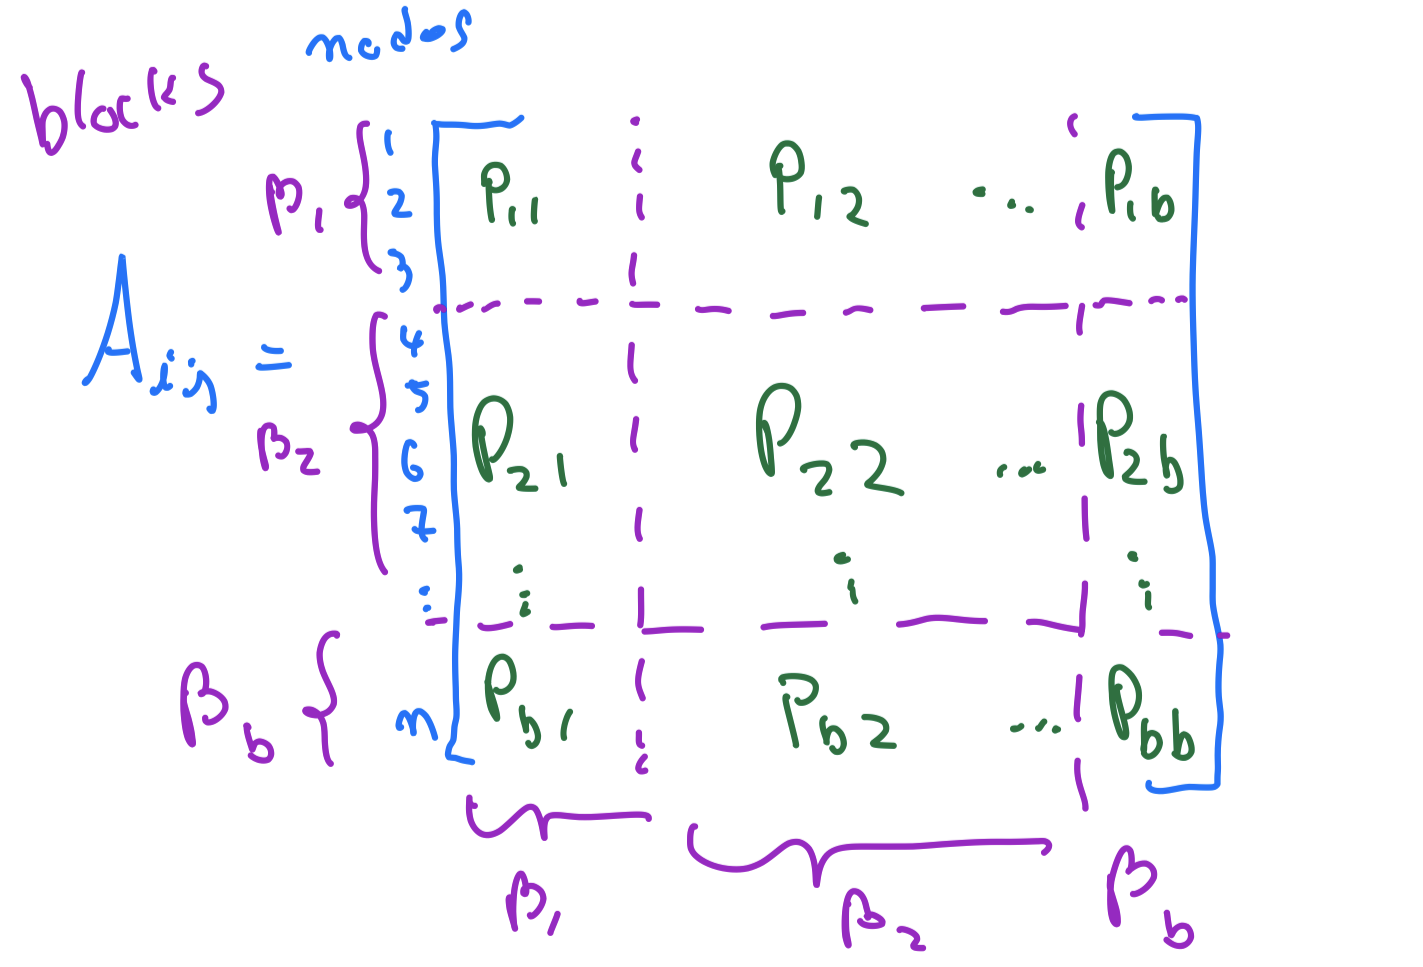
\includegraphics[scale=0.4]{SBM}
\end{center}

We now show that the SBM is a generalisation of models we have seen previously.

\begin{lemma}(Poisson Random Graph). Suppose that we only have 1 block $B = 1$ in our network. Then, $p_{r,s} = p$ for all blocks $\beta_r, \beta_s \in \tilde{\beta}$. Therefore, we have a Poisson Random Graph.
\end{lemma}

\begin{lemma}(Bipartite Graph). Suppose that we have 2 blocks $B = 2.$ Let $p_{11} = p_{22} = 0$ and $p_{12} \neq 0$ and $p_{21} \neq 0.$ Then, we only have links between blocks. Therefore, we have a Bipartite graph.
\end{lemma}

\begin{lemma}(Modular network). Suppose that we have B blocks. Now, set the probability of links to be 
$$
p_{r,s} = 
\begin{cases}
\epsilon \quad r \neq s \\
p >> \epsilon \quad r = s
\end{cases}
$$
Therefore, we have a modular networks where we have more links within communities than across communities.
\end{lemma}


Now that we have described the generative process, we want to work backwards. That is, given the adjacency matrix of our network, what are the block assignments? Therefore, we are now interested in computing the likelihood for a given realisation of a graph g with adjacency matrix $A.$

\begin{definition_exam}{Likelihood of a network}{}Let g be a simple graph and A its associated adjacency matrix. Then, the likelihood of the graph g is given by 
$$
p(g) = p(A) = \prod_{r,s}\prod_{j = \beta_{s}}\prod_{i = \beta_{r}}p_{r,s}^{A_{i,j}}(1 - p_{r,s})^{1 - A_{i,j}}
$$
\end{definition_exam}

\begin{remark}The probability of a graph is the probability of each edge of the graph as the edges are independent of one another.
\end{remark}

We are now interested in the case for when we know the block assignments and the harder case for when we don't know the block assignment.

\begin{proposition_exam}{SBM likelihood under known block assignment}{}Suppose that we have a graph g with adjacency matrix A. Furthermore, assume that the block assignment for each node is known $\tilde{b} = \{b_1,...,b_N\}$. Then, the likelihood of the graph g is given by 
$$
p(g) = \prod_{r,s}p_{r,s}^{\ell_{r,s}}(1 - p_{r,s})^{m_{r,s} - \ell_{r,s}}
$$
where $\ell_{r,s}$ is the number of links between block r and s 
$$
\ell_{r,s} = \sum_{\substack{i = \beta_r \\ j = \beta_s}}A_{i,j}
$$
and $m_{r,s}$ is the maximum number of links between block r and s.
\end{proposition_exam}

\begin{remark}$m_{r,s} - \ell_{r,s}$ can be interpreted as the number of 0's in the adjacency matrix between block r and s.
\end{remark}

\begin{corollary}Suppose that we have a graph g with adjacency matrix A. Furthermore, assume that the block assignment for each node is known $\tilde{b} = \{b_1,...,b_N\}$. Then, the parameter $p_{r,s}$ can be computed by maximizing 
\begin{equation}
p(g) = \prod_{r,s}p_{r,s}^{\ell_{r,s}}(1 - p_{r,s})^{m_{r,s} - \ell_{r,s}}.
\tag{*}
\end{equation}
Furthermore, as $p_{r,s}$ is independent of each other, the maximization of equation (*) is equivalent to the maximization of each term $p_{r,s}.$ The estimator of each term $p_{r,s}$ is given by 
$$
\hat{p_{r,s}} = \frac{\ell_{r,s}}{m_{r,s}} = \text{fraction of possible links}
$$
\end{corollary}


Now, we look at the harder case of what to do when the block assignmnet $\tilde{b}$ is unknown. The reason that this is hard is that there is an exponential number of possible block assignments.
\begin{lemma}The number of possible block assignments is $B^N$ where N is the number of nodes and B is the number of block labels.
\end{lemma}
We can therefore see it is difficult when we do not know the block assignment. However, what we can do is fix a given block assignment $\tilde{b}$ and then maximize the likelihood
$$
p(g) = \prod_{r,s}p_{r,s}^{\ell_{r,s}}(1 - p_{r,s})^{m_{r,s} - \ell_{r,s}}
$$
But again, we saw that we can have an exponential number of block assignments to go through in order to find the optimal assignment. 

\begin{proposition}Suppose we have a block assignment $\tilde{b}.$ We can take negative logarithm of the likelihood function in order to derive the negative log-likelihood
$$
-log(p(g)) = -\sum_{r, s}\bigg(\ell_{r,s}log\;p_{r,s} + (m_{r,s} - \ell_{r,s})log(1 - p_{r,s}) \bigg)
$$
where 
$$
p_{r,s} = \frac{\ell_{r,s}}{m_{r,s}}.
$$
is the fraction of observed actual edges between block r and s.
\end{proposition}

\begin{corollary}
Maximizing the likelihood is equivalent to minimising the negative log-likelihood.
\end{corollary}

We can see that in the SBM set up, our model has parameters $B, \tilde{b}, p_{r,s}.$ Furthermore, the dataset involves each link as each link is conditionally independent of each other.

Alot of SBMs detect a core-periphery structure (all hubs in one block and leaves in another).

\begin{remark}The degree corrected SBM is when 
$$
p_{rs} \sim Z_iZ_j\lambda_{r,s}
$$
where $Z_i$ is the degree of node i and $Z_j$ is the degree of node j where $b_i = \beta_r$ and $b_j = \beta_s$
\end{remark}

It is difficult to even know what value of B to use. Therefore, an approach we can also take is to set hyperpriors on the number of blocks p(B). 

\lecture{21}{Computational Inference Techniques}
\section{Statistical Models}
\subsection{Computational Inference Techniques}
\begin{definition}(Statistical inference). Let D be the data and M the models with parameters $\theta.$ The goal of statistical inference is to learn the properties of the underlying probabilistic models.
\end{definition}

We now describe the frequentist approach.
\begin{definition}(Frequentist approach). The frequentist involves working with the likelihood function 
$$
\mathcal{L} = p(D|M)
$$
where the models M and parameter $\theta$ is selected based on the maximum likelihood principle.
\end{definition}

\begin{definition_exam}{Bayesian approach}{} Using Bayes theorem, we define the posterior distribution of our model to be
$$
p(M|D) = \frac{p(D|M)p(M)}{p(D)}
$$
where $p(M)$ is the prior and p(D) is the evidence.
\end{definition_exam}

\begin{remark}Maximizing the posterior distribution only requires maximizing the numerator $p(D|M)p(M)$ as the evidence p(D) is fixed.
\end{remark}

However, we have a few computational issues.
\begin{enumerate}
\item The likelihoods and posterior distributions are intractable;
\item We have a high dimensional parameter space $e^{\alpha N}$ and therefore exhaustive searches are infeasible.
\end{enumerate}

Therefore, we require smarter approaches.

\begin{definition}(Kullback-Leibler Divergence). Let p and q be probability density functions. Then, the KL-divergence is given by 
$$
KL(q||p) = H(p) - H(q|p) = \sum_xp\;logp - \sum_xp\;logq
$$
\end{definition}

\begin{proposition_exam}{Variational Inference}{} Suppose $p(M|D)$ is the intractable likelihood or posterior distribution of interest. Then, propose a family of tractable density functions $q(M) \subset D$ that approximates $p(M|D)$ and therefore we seek to minimise the distance 
$$
q^*(M) = \min_{q(M) \subset D}KL(q(M)||p(M|D))
$$
\end{proposition_exam} 

\begin{remark}Variational inferences scales well but it depends heavily on the choice of the family of density functions we use. If functions that we choose to approximate with are good, then we get a good result. However, variational inference can give us bad results if we pick a bad family.
\end{remark}

We now specify the MCMC method for SBM.

\begin{proposition_exam}{MCMC Method for block assignment}{}Denote $\tilde{b}$ to be a block assignment. We can specify the transformation $T(\tilde{b})$ to be changing the block allocation of a single node. Then 
$$
\pi(\tilde{b} \rightarrow \tilde{b^{'}}) = \pi(\tilde{b^{'}} \rightarrow \tilde{b})
$$
Therefore, we have the Metropolis-Hastings acceptance to be 
$$
A(b \rightarrow b^{'}) = 
\min \{1, \frac{e^{log\;\mathcal{L}(b)}}{e^{log\;\mathcal{L}(b^{'})}} \}
= 
\begin{cases}
1 \quad -\Delta log\;\mathcal{L} < 0 \\
e^{\Delta log\;\mathcal{L}} \quad -\Delta log\;\mathcal{L} > 0 \\
\end{cases}
$$
Therefore, as $t \rightarrow \infty,$ we have that $\tilde{b}$ is sampled from $\mathcal{L}(\tilde{b}).$
\end{proposition_exam}

We may also add an inverse temperate where $\beta = \frac{1}{T}$ and therefore, as $\beta = 0,$ we have that A = 1 and therefore we get a random walk. However, as $\beta \rightarrow \infty,$ we get a Greedy algorithm.

Furthermore, we can sample from the likelihood $\mathcal{L}(\beta)$ using the importance sampling algorithm.


\begin{remark}The greedy and variational inference methods will be trapped in the local minima. However, the MCMC algorithm will not be trapped as $T \rightarrow \infty$ as it samples from the whole distribution as it equilibrates. 
\end{remark}

Higher levels of $\beta,$ will help us to escape local minima and explore different levels of the phase space.
\begin{proposition}(Simulated Annealing). The idea is to start with a small temperature $\beta = 0$. Then, we equilibrate the MCMC chains. We then increase the temperature $\beta$ and repeat.
\end{proposition}


\lecture{22}{Graph Bisection and Modularity Maximization}
\section{Communities}
\section{Communities}


We now investigate alternative approaches to community detection in networks. Again, our intuition is that for communities, we expect more links within a community compared to having links across communities. The goal of community detection is to identify the communities and partitions based only on the connectivity and the links in the network. However, this is not trivial due to the high dimensional parameter space. 

There are two aspects of community detection.
\begin{enumerate}
\item Find the best partition of the network 
\item Learn about the process that generated the network
\end{enumerate}

Some methods are good at the first task whilst others are better at the second task. We note that by the No Free Lunch theorem, there is not a single method that excels at both tasks.

We now state on why is it hard to figure out the community structure of a network.
\begin{proposition_exam}{The number of possible community partitions is exponential}{}The number of possible partitions of N vertices into B communities can be given by the Bell number
$$
Be(N) = \sum_{B=1}^{N}S(N,B) 
$$
where $S(N,B)$ is the Stirling number of the second type.
\end{proposition_exam}

\begin{remark}We note that the Bell number grows faster than an exponential growth. Furthermore, note that we have at most N blocks.
\end{remark}

Now, before we proceed further, we describe some implicit assumptions made in our methods to infer the community structure. 

\begin{definition_exam}{Fundamental Hypothesis}{} A network's community structure is uniquely encoded in its adjacency matrix $\utilde{A}.$
\end{definition_exam}
\begin{remark} This states that it is not only the degree distribution of the network but the way in which nodes are linked to one another which determines the communities.
\end{remark}

\begin{definition_exam}{Connectedness Hypothesis}{}Each community corresponds to a connected subgraph of the network.
\end{definition_exam}
\begin{remark} Consequently, if a network consists of two isolated components, each community is limited to only one component. The hypothesis also implies that on the same component a community cannot consist of two subgraphs that do not have a link to each other. 
\end{remark}

\begin{definition_exam}{Density Hypothesis}{}Nodes in a community are more likely to connect to other members of the same community than to nodes in other communities.
\end{definition_exam}

\subsection{Graph Bisection}
The goal of graph partitioning is to minimize the number of links between communities. This is otherwise known as the cut size.

The key simplifying assumption is that that we know the number of communities B and the sizes of each community $N_1,N_2,...,N_B$ are pre-specified.


\begin{lemma}(Graph partitioning is NP-hard). There does not exist a polynomial time algorithm to find all possible partitions. That is, searching the parameter space of possible partitions is NP-hard.
\end{lemma}

The goal is to find a good partition of the network in polynomial time. We desscribe an algorithm to find a good partition for when we have two communities.

\begin{algorithm}
\DontPrintSemicolon
\KwIn{B = 2 communities}
Start with random partitions of nodes into B = 2 communities of size $N_1$ and $N_2$\;
For all pair of nodes, identify the swaps of community assignment that minimises the cut size\;
Perform swaps for all swaps which decreases the cut size are performed\;
Pick the minimal cut-size\;
\Return{Partition of nodes into B = 2 communities of size $N_1$ and $N_2$}\;
\caption{{\sc Kernighan-Lin Algorithm}}
\label{algo:duplicate}
\end{algorithm}

\begin{proposition}(Kernighan-Lin Algorithm). The computational complexity of the Kernighan-Lin algorithm is $\mathcal{O}(N^2).$
\end{proposition}

\begin{remark}A limitation of the Kernighan-Lin algorithm is that we cannot extend it to finding the number of communities B. Furthermore, it does not tell us what should the size of the two communities $N_1, N_2$ should be.
\end{remark}

\subsection{Modularity Maximization}

We want to extend on the ideas from the last section. We want to find a quantity such that when optimized, figures out the number of communities B and assign community labels $b_i \subset \{\beta_1,...,\beta_B\}$ for all nodes i.

\begin{definition_exam}{Number of links within a community}{}
The number of links within a community is defined to be
$$
L_1 = \sum_{\text{edges (i,j)}}\delta(b_i, b_j) = \frac{1}{2}\sum_{j=1}^{N}\sum_{i=1}^{N}A_{ij}\delta(b_i, b_j)
$$
where $\delta(b_i, b_j)$ is an indicator for when two nodes are within the same community.
\end{definition_exam}

We now want to compute the expected number of links, as this gives us a probabilistic formulation of what do we expect by chance. We need to take into account of randomness in the model. The probability of a connection between node i and node j is 
$$
p_{ij} = \frac{z_iz_j}{2L}
$$
where L is the number of edges in the network and $Z_k$ is the degree of node k. This is inspired by the configuration model.

\begin{definition_exam}{Expected number of links within a community}{}The expected number of links within a community is defined to be
$$
L_2 = \frac{1}{2}\sum_{i=1}^{N}\sum_{j=1}^{N}\frac{z_iz_j}{2L}\delta(b_i, b_j)
$$
where $\delta(b_i, b_j)$ is an indicator for when two nodes are within the same community and $z_k$ is the degree of node k.
\end{definition_exam}

We can now define the quality function of interest which we seek to maximize.

\begin{definition_exam}{Modularity}{}The modularity of an assignment of community labels is given by the modularity 
$$
Q = \frac{L_1 - L_2}{L} = \frac{1}{2L}\sum_{i=1}^{N}\sum_{j=1}^{N}\bigg(A_{ij} - \frac{z_iz_j}{2L} \bigg)\delta(b_i, b_j)
$$
where L is the total number of edges in the network.
\end{definition_exam}

\begin{corollary} We give another definition of modularity by 
$$
Q = \sum_{c=1}^{n_c}\bigg[\frac{L_c}{L} - \bigg(\frac{z_c}{2L} \bigg)^2 \bigg]
$$
where $L_c$ is the number of links within community $C_c,$ $n_c$ is the number of nodes in community $C_c,$ $z_c$ is the total degree of nodes in community $C_c,$ and L is the total number of links in the network.
\end{corollary}

\begin{remark}We see that modularity does not give us trivial results. If B = 1, then we have that all nodes are in the same community and we will have a modularity of Q = 0. Now, suppose that B = N, then we will have that $Q < 0.$ Therefore, B is chosen by maximizing the Q and will be a non-trivial result as we just saw.
\end{remark}

Again, we are unable to exhaustively search all possible partitions of B. However, there are 2 main approaches to maximize the modularity Q and the number of communities.
\begin{enumerate}
\item Agglomerative methods: We start off with every node in its own community. We then merge communities that gives us the greatest increase in modularity until we end up with only 1 community.
\item Divisive methods: We start off with one community for the whole network. We then split nodes into separate communities depending on what gives us the greatest increase in modularity. We continue until every node is in its own community.
\end{enumerate}

We state the Greedy Agglomerative approach in more detail.

\begin{algorithm}
\DontPrintSemicolon
\KwIn{B = N communities}
$B \gets N$ where each node is in its own community\;
Check all possible merges\;
$\Delta Q \gets Q - Q^{'}$ choose the merger that maximizes the difference $\Delta Q$\;
$\tilde{B}^{'} \gets \tilde{B}$ is a new partition where number of communities decrements $B \rightarrow B - 1$\;
Repeat step 2-3 until you end up with $B = 1$ community\;
\Return{Partition of nodes into B = 2 communities of size $N_1$ and $N_2$}\;
\caption{{\sc Greedy Agglomerative Method}}
\label{algo:duplicate}
\end{algorithm}

From the above algorithm, choose the $B = B^*$ that maximizes the modularity and hence gives us the optimal partition.

\begin{proposition}The computational complexity of the Greedy Agglomerative method is $\mathcal{O}(N^2).$
\end{proposition}

\begin{center}
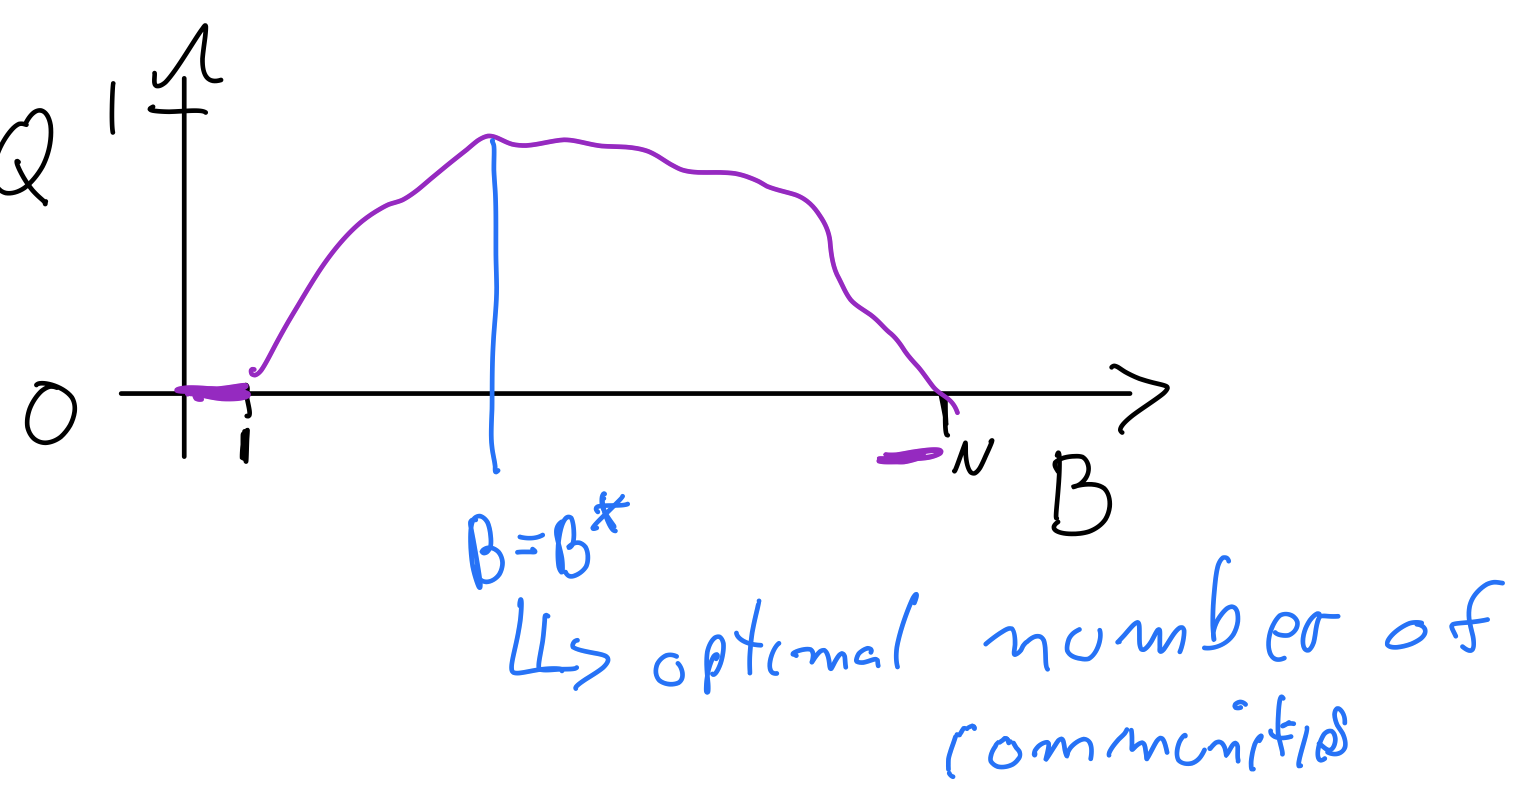
\includegraphics[scale=0.4]{Modularity}
\end{center}


\begin{remark}It is important to note that the Greedy Agglomerative approach and the Greedy Divisive approach will not necessarily give us the same result.
\end{remark}

There are ways we can improve the runtime of the algorithm. First, we can store links within and across communities. Furthermore, we can only try merges between communities that are linked to each other. From these improvements, we can improve our runtime to a $\mathcal{O}(N\;log^2\;N)$ runtime.

There are many alternative methods for modularity maximization which includes the 
\begin{enumerate}
\item Louvain method: Start with small communities and grow communities based off this.
\item Simulated annealing: Introduce a temperature which we can adjust to alter our results in the optimization result.
\item There are also ways to generalise the modularity function Q.
\end{enumerate}

\lecture{23}{Community Detection Alternatives}
\section{Communities}
\subsection{Spectral Methods}
We now are interested in using methods that involves the spectrum of matrices.

\begin{definition}(Laplacian Matrix). The Laplace matrix of a network with N nodes is given by
$$
\mathcal{L} = D - A
$$
where D is a N-by-N diagonal matrix where diagonal entry j represents the degree $Z_j$ of node j and A is the adjacency matrix associated to the network.
\end{definition}

Now, recall some linear algebra.
\begin{definition}(Eigenvalue and eigenvector). For a matrix A, $\lambda$ is an eigenvalue of A if for some vector v, we have that 
$$
A v = \lambda v
$$
where v is the eigenvector of A corresponding to $\lambda.$
\end{definition}

\begin{theorem_exam}{Spectrum of the Laplace Matrix}{}The Laplace matrix $\mathcal{L}$ of the network has K eigenvalues $\{\lambda_1, \lambda_2, ..., \lambda_K\}$ and associated eigenvectors $\{v_1, v_2, ..., v_k\}$.
\end{theorem_exam}

\begin{proposition}Suppose that the Laplace matrix $\mathcal{L}$ has K eigenvalues where 
$$
\lambda_1 = \lambda_2 = ... = \lambda_K = 0.
$$
Then, the network has K connected components.
\end{proposition}

With our K components, we can perturb the configuration by adding links between components. From this, the eigenvalues $\lambda_i \geq 0$ for i = 1,...,K. Then, the goal is to chose B (the number of communities) to be the number of eigenvectors that are close to zero.

Hence, we can cluster the vectors associated to the Laplace matrix by using the K-means clustering method.

\begin{remark}Other matrices can be used instead of the Laplace matrix. One example is the Modularity matrix 
$$
M_{ij} = A_{ij} - \frac{Z_iZ_j}{L}
$$
\end{remark}

\subsection{Label Propagation Methods}
We analyse processes taking place in the network and analyse where does the trajectory of these processes in the networks lead to. The intuition behind the Label Propagation Algorithm is that a single label can quickly become dominant in a densely connected group of nodes, but will have trouble crossing a sparsely connected region. Labels will get trapped inside a densely connected group of nodes, and those nodes that end up with the same label when the algorithms finish can be considered part of the same community.



The algorithm works as follows:
\begin{enumerate}
\item Every node is initialized with a unique community label (an identifier).
\item These labels propagate through the network.
\item At every iteration of propagation, each node updates its label to the one that the maximum numbers of its neighbours belongs to. Ties are broken uniformly and randomly.
\item LPA reaches convergence when each node has the majority label of its neighbours.
\item LPA stops if either convergence or the user-defined maximum number of iterations is achieved.
\end{enumerate}

\end{document}

}
}

